\documentclass[twoside]{book}

% Packages required by doxygen
\usepackage{fixltx2e}
\usepackage{calc}
\usepackage{doxygen}
\usepackage[export]{adjustbox} % also loads graphicx
\usepackage{graphicx}
\usepackage[utf8]{inputenc}
\usepackage{makeidx}
\usepackage{multicol}
\usepackage{multirow}
\PassOptionsToPackage{warn}{textcomp}
\usepackage{textcomp}
\usepackage[nointegrals]{wasysym}
\usepackage[table]{xcolor}

% Font selection
\usepackage[T1]{fontenc}
\usepackage[scaled=.90]{helvet}
\usepackage{courier}
\usepackage{amssymb}
\usepackage{sectsty}
\renewcommand{\familydefault}{\sfdefault}
\allsectionsfont{%
  \fontseries{bc}\selectfont%
  \color{darkgray}%
}
\renewcommand{\DoxyLabelFont}{%
  \fontseries{bc}\selectfont%
  \color{darkgray}%
}
\newcommand{\+}{\discretionary{\mbox{\scriptsize$\hookleftarrow$}}{}{}}

% Page & text layout
\usepackage{geometry}
\geometry{%
  a4paper,%
  top=2.5cm,%
  bottom=2.5cm,%
  left=2.5cm,%
  right=2.5cm%
}
\tolerance=750
\hfuzz=15pt
\hbadness=750
\setlength{\emergencystretch}{15pt}
\setlength{\parindent}{0cm}
\setlength{\parskip}{3ex plus 2ex minus 2ex}
\makeatletter
\renewcommand{\paragraph}{%
  \@startsection{paragraph}{4}{0ex}{-1.0ex}{1.0ex}{%
    \normalfont\normalsize\bfseries\SS@parafont%
  }%
}
\renewcommand{\subparagraph}{%
  \@startsection{subparagraph}{5}{0ex}{-1.0ex}{1.0ex}{%
    \normalfont\normalsize\bfseries\SS@subparafont%
  }%
}
\makeatother

% Headers & footers
\usepackage{fancyhdr}
\pagestyle{fancyplain}
\fancyhead[LE]{\fancyplain{}{\bfseries\thepage}}
\fancyhead[CE]{\fancyplain{}{}}
\fancyhead[RE]{\fancyplain{}{\bfseries\leftmark}}
\fancyhead[LO]{\fancyplain{}{\bfseries\rightmark}}
\fancyhead[CO]{\fancyplain{}{}}
\fancyhead[RO]{\fancyplain{}{\bfseries\thepage}}
\fancyfoot[LE]{\fancyplain{}{}}
\fancyfoot[CE]{\fancyplain{}{}}
\fancyfoot[RE]{\fancyplain{}{\bfseries\scriptsize Generated by Doxygen }}
\fancyfoot[LO]{\fancyplain{}{\bfseries\scriptsize Generated by Doxygen }}
\fancyfoot[CO]{\fancyplain{}{}}
\fancyfoot[RO]{\fancyplain{}{}}
\renewcommand{\footrulewidth}{0.4pt}
\renewcommand{\chaptermark}[1]{%
  \markboth{#1}{}%
}
\renewcommand{\sectionmark}[1]{%
  \markright{\thesection\ #1}%
}

% Indices & bibliography
\usepackage{natbib}
\usepackage[titles]{tocloft}
\setcounter{tocdepth}{3}
\setcounter{secnumdepth}{5}
\makeindex

% Hyperlinks (required, but should be loaded last)
\usepackage{ifpdf}
\ifpdf
  \usepackage[pdftex,pagebackref=true]{hyperref}
\else
  \usepackage[ps2pdf,pagebackref=true]{hyperref}
\fi
\hypersetup{%
  colorlinks=true,%
  linkcolor=blue,%
  citecolor=blue,%
  unicode%
}

% Custom commands
\newcommand{\clearemptydoublepage}{%
  \newpage{\pagestyle{empty}\cleardoublepage}%
}

\usepackage{caption}
\captionsetup{labelsep=space,justification=centering,font={bf},singlelinecheck=off,skip=4pt,position=top}

%===== C O N T E N T S =====

\begin{document}

% Titlepage & ToC
\hypersetup{pageanchor=false,
             bookmarksnumbered=true,
             pdfencoding=unicode
            }
\pagenumbering{alph}
\begin{titlepage}
\vspace*{7cm}
\begin{center}%
{\Large notepad }\\
\vspace*{1cm}
{\large Generated by Doxygen 1.8.13}\\
\end{center}
\end{titlepage}
\clearemptydoublepage
\pagenumbering{roman}
\tableofcontents
\clearemptydoublepage
\pagenumbering{arabic}
\hypersetup{pageanchor=true}

%--- Begin generated contents ---
\chapter{说明文档}
\label{index}\hypertarget{index}{}\section*{基于\+M\+F\+C的文本编辑器 }

\subsection*{目标 }


\begin{DoxyEnumerate}
\item 不使用\+M\+F\+C文本框控件,实现一个简单的文本编辑器
\item 最低要求如下: 带有图形界面 能够比较方便的给不同的字符设置不同的字体、颜色和字号 可以设置字与字之间的间距
\item 另外还实现了以下功能 保存、打开自定义格式的文件 设置对齐方式,包括左对齐、居中对齐、右对齐、分散对齐 设置行间距
\end{DoxyEnumerate}

\subsection*{使用方法 }


\begin{DoxyEnumerate}
\item 常规操作与普通文本编辑器相同
\item 设置字体、颜色、字号:
\begin{DoxyItemize}
\item 选中想要改变的文本内容
\item 点击编辑菜单栏,点击字体,将会弹出选择字体的窗口
\item 选择想要设置的格式即可
\end{DoxyItemize}
\item 设置对齐方式:
\begin{DoxyItemize}
\item 如果只需要设置单行的格式,请直接将光标移到该行
\item 如果需要设置多行的格式,请选中多行
\item 点击编辑菜单栏,点击对齐方式
\item 在弹出的右侧菜单栏中选择需要的对齐方式
\end{DoxyItemize}
\item 设置行间距、字间距:
\begin{DoxyItemize}
\item 选中需要设置的文本内容
\item 点击编辑菜单栏,点击段落
\item 在弹出的窗口中输入需要设置的行间距以及字间距
\item 注意单位为像素
\end{DoxyItemize}
\item 打开与保存
\begin{DoxyItemize}
\item 首先注意,本文本编辑器只支持自定义格式的(后缀名为$<$tt$>$.\+orz)文件,其他格式的文件一律无法打开
\item 打开:点击菜单栏,点击打开,在文件浏览器中选择想要打开的文件,点击确定即可
\item 保存:点击菜单栏,点击保存,在文件浏览器中选择想要保存的目录,点击确定即可
\end{DoxyItemize}
\end{DoxyEnumerate}

\subsection*{构件库 }

详情请参见\+Class List

\subsection*{U\+I界面的交互实现方法说明 }


\begin{DoxyEnumerate}
\item 设置字体字号颜色 ~\newline
通过{\ttfamily C\+Font\+Dialog}窗口类,创建选择字体的窗口 ~\newline
用户选择字体以及颜色后,获取字体信息{\ttfamily L\+O\+G\+F\+O\+NT}以及颜色信息{\ttfamily R\+E\+F\+C\+O\+L\+OR}~\newline
通过{\ttfamily set\+\_\+select\+\_\+font}与{\ttfamily set\+\_\+select\+\_\+col}函数将字体以及颜色信息传递给后端~\newline

\item 设置字间距行间距 ~\newline
通过{\ttfamily \hyperlink{class_m___p_a_r_a___d_i_a}{M\+\_\+\+P\+A\+R\+A\+\_\+\+D\+IA}}对话框,获取用户设置的字间距与行间距的值 ~\newline
通过{\ttfamily set\+\_\+select\+\_\+lspace}与{\ttfamily set\+\_\+select\+\_\+cspace}函数将字间距与行间距传给后端~\newline

\item 保存、打开文件 ~\newline
通过{\ttfamily C\+File\+Dialog}类,返回用户需要保存或者打开文件的路径~\newline
通过{\ttfamily \#}与{\ttfamily \#}函数将路径作为字符串传给后端~\newline

\item 设置对齐方式 ~\newline
直接通过消息响应函数,调用{\ttfamily set\+\_\+select\+\_\+align}函数,设置对齐方式~\newline

\end{DoxyEnumerate}

\subsection*{后端(kernal)实现方法说明 }


\begin{DoxyEnumerate}
\item 抽象~\newline

\begin{DoxyItemize}
\item 把画在屏幕上的字符看作一个矩形~\newline

\item 用链表从前往后储存字符~\newline

\end{DoxyItemize}
\item 计算绘制信息~\newline

\begin{DoxyItemize}
\item 遍历文本链表,进行预处理~\newline

\item 遍历文本链表,把链表分成很多行~\newline

\begin{DoxyItemize}
\item 当某行的字符宽度之和({\ttfamily tot\+\_\+width})将要超过页面宽度({\ttfamily pagewidth})时,开一个新行~\newline

\item 当遇到换行符时,开一格新行~\newline

\end{DoxyItemize}
\item 从上往下遍历每一行,根据相关信息计算该行内的{\ttfamily n}个字符矩形的位置~\newline

\begin{DoxyItemize}
\item 如果该行是默认对齐方式或者左对齐,那么x坐标从0开始,每个矩形宽度加上字间距,从左往右计算~\newline

\item 如果该行是右对齐,那么x坐标从{\ttfamily pagewidth}-\/{\ttfamily tot\+\_\+width}开始,每个矩形宽度加上字间距,从左往右计算~\newline

\item 如果对齐方式是居中对齐,那么x坐标从({\ttfamily pagewidth}-\/{\ttfamily tot\+\_\+width})/2开始,每个矩形宽度加上字间距,从左往右计算~\newline

\item 如果对齐方式是分散对齐,那么x坐标从0开始,每个矩形宽度加上字间距和{\ttfamily delta}=({\ttfamily pagewidth}-\/{\ttfamily tot\+\_\+width})/{\ttfamily n}~\newline

\end{DoxyItemize}
\end{DoxyItemize}
\end{DoxyEnumerate}

\subsection*{U\+I及交互部分遇到的问题及解决方案 }


\begin{DoxyEnumerate}
\item 绘图过程闪烁的问题 ~\newline
问题描述:使用过程中每当需要屏幕刷新的时候,画面会不停的闪烁 ~\newline
可能原因:每次调用\+On\+Paint函数的时候都会先将屏幕清空,由于绘制屏幕仍然需要一定的时间,所以每次重绘都会出现闪烁的情况 ~\newline
解决方案:使用双缓冲绘图,分为两个部分:~\newline
(1)重载{\ttfamily B\+O\+OL \hyperlink{class_c_child_view_a6060e6d09d522d345dcee5a01d41c1f0}{C\+Child\+View\+::\+On\+Erase\+Bkgnd(\+C\+D\+C$\ast$ p\+D\+C)}}函数,使得画面不会被擦除~\newline
(2)先在使用内存\+D\+C上画图,画好后直接调用{\ttfamily Bit\+Blt}函数将画面传给物理\+DC~\newline

\item 滚动条位置以及大小的问题~\newline
问题描述:滚动条大小以及位置随着窗口大小改变而随机变动~\newline
可能原因:由于滚动条控件需要手动设置大小以及位置,所以当改变窗口大小的时候会出现滚动条位置偏移的情况~\newline
解决方案:设置两个变量:{\ttfamily m\+\_\+client\+\_\+cy}记录页面长度,{\ttfamily scrolledpix}记录页面相对于窗口上端的偏移量~\newline
每次重绘的时候通过这两个量来重新计算滚动条的大小以及位置~\newline

\item 解析用户传入的键盘消息~\newline
问题描述:根据官方文档,键盘消息的对应关系很复杂,需要解析传入的参数才能获得字符信息~\newline
解决方案:使用{\ttfamily void \hyperlink{class_c_child_view_af29ede94259b52b2ad54d139ff554abe}{C\+Child\+View\+::\+On\+Char(\+U\+I\+N\+T n\+Char, U\+I\+N\+T n\+Rep\+Cnt, U\+I\+N\+T n\+Flags)}}的消息响应函数~\newline
系统将键盘消息处理后返回用户输入的字符~\newline

\item 连按消息的问题~\newline
问题描述:通常连按一个按键,被认为是连续输入字符~\newline
解决方案:在{\ttfamily void \hyperlink{class_c_child_view_a74d87512b76128e2eedea87811363e45}{C\+Child\+View\+::\+On\+Key\+Down(\+U\+I\+N\+T n\+Char, U\+I\+N\+T n\+Rep\+Cnt, U\+I\+N\+T n\+Flags)}}函数中~\newline
{\ttfamily n\+Rep\+Cnt}参数是用于标记连按消息的次数的,循环相应的次数即可实现连续输入~\newline

\item 获取字体的像素大小的问题~\newline
问题描述:{\ttfamily L\+O\+G\+F\+O\+NT}结构体的成员{\ttfamily lf\+Height}与{\ttfamily lf\+Width}不是像素高度~\newline
解决方案:通过公式{\ttfamily pix\+Height = -\/(lf\+Height $\ast$ 72) / Get\+Device\+Caps(h\+D\+C,\+L\+O\+G\+P\+I\+X\+E\+L\+S\+Y)}转换为像素高度~\newline
参考资料:\href{https://msdn.microsoft.com/zh-cn/library/bb773327.aspx}{\tt M\+S\+D\+N上关于\+L\+O\+G\+F\+O\+N\+T的说明}~\newline

\end{DoxyEnumerate}

\subsection*{后端(kernal)遇到的问题及解决方案 }


\begin{DoxyEnumerate}
\item 空行的问题~\newline
问题描述:链表中换行符只用作开启一行的标识符,如果用户连续键入两个换行,第二个换行会变成\char`\"{}空行\char`\"{}而无法在屏幕上打出来~\newline
解决方案:在预处理中,先遍历链表,在相邻两个换行符之间插入一个{\ttfamily S.\+width}=0,{\ttfamily size}=-\/1的字符,避免\char`\"{}空行\char`\"{}的产生~\newline

\item 使用\char`\"{}打开\char`\"{}命令后单击屏幕会崩溃的问题~\newline
问题描述:添加\char`\"{}打开\char`\"{}模块后,用户在界面上单击会导致崩溃~\newline
问题原因:执行\char`\"{}打开\char`\"{}命令后,后端的选中信息会丢失,而\+U\+I当作用户\char`\"{}完成\char`\"{}了一次选中操作调用了{\ttfamily end\+\_\+select}函数,导致内存无效访问~\newline
解决方案:在对选中区域执行任何操作前,先检查是否存在选中区域~\newline

\item \char`\"{}打开\char`\"{}命令对于某些字体无法执行的问题~\newline
问题描述:当打开包含字体名称({\ttfamily lf\+Face\+Name})为多个单词的文件时,\char`\"{}打开\char`\"{}操作会失败~\newline
问题原因:字体名称是{\ttfamily wchar\+\_\+t}类型的,最初我用的scanf(\char`\"{}\%ls\char`\"{})来读取字体名称,这样就只能读到字体名称的第一个单词,而且我没有找到~\newline
针对{\ttfamily wchar\+\_\+t}数组的getline函数。 解决方案:手写针对{\ttfamily wchar\+\_\+t}的{\ttfamily si\+\_\+getline}函数~\newline
 \subsection*{测试用例 }
\end{DoxyEnumerate}


\begin{DoxyEnumerate}
\item {\ttfamily align.\+orz}:测试四种对齐方式
\item {\ttfamily keepcalm.\+orz}:测试设置字体、字号、颜色
\item {\ttfamily linechaspace.\+orz}:测试设置行间距、字间距
\end{DoxyEnumerate}

\subsection*{总结 }


\begin{DoxyEnumerate}
\item 程序具有一定的可使用性,实现了基本目标,在数据规模不太大的情况下可以达到较好效果
\item 当数据规模较大时(超过50000字符),会出现明显的卡顿现象,所以程序仍然有很大改进空间 可以通过每次只计算、绘制当前屏幕附近的字符来解决这个问题
\end{DoxyEnumerate}

\subsection*{作者信息 }


\begin{DoxyItemize}
\item kernal部分作者:李仁杰~\newline

\begin{DoxyItemize}
\item 学院:清华大学软件学院~\newline

\item 班级:软件62~\newline

\item 学号:2016013271~\newline

\item e-\/mail:\+Shadow\+Iterator@hotmail.\+com~\newline

\item 电话:18801005736~\newline

\end{DoxyItemize}
\item U\+I及交互部分作者:洪方舟~\newline

\begin{DoxyItemize}
\item 学院:清华大学软件学院~\newline

\item 班级:软件62~\newline

\item 学号: 2016013259~\newline

\item e-\/mail\+: \href{mailto:hongfz16@163.com}{\tt hongfz16@163.\+com}~\newline

\item 电话:15062727188~\newline

\end{DoxyItemize}
\end{DoxyItemize}
\chapter{Hierarchical Index}
\section{Class Hierarchy}
This inheritance list is sorted roughly, but not completely, alphabetically\+:\begin{DoxyCompactList}
\item C\+Dialog\+Ex\begin{DoxyCompactList}
\item \contentsline{section}{C\+About\+Dlg}{\pageref{class_c_about_dlg}}{}
\item \contentsline{section}{M\+\_\+\+P\+A\+R\+A\+\_\+\+D\+IA}{\pageref{class_m___p_a_r_a___d_i_a}}{}
\end{DoxyCompactList}
\item C\+Frame\+Wnd\begin{DoxyCompactList}
\item \contentsline{section}{C\+Main\+Frame}{\pageref{class_c_main_frame}}{}
\end{DoxyCompactList}
\item C\+Win\+App\begin{DoxyCompactList}
\item \contentsline{section}{C\+Notepad\+App}{\pageref{class_c_notepad_app}}{}
\end{DoxyCompactList}
\item C\+Wnd\begin{DoxyCompactList}
\item \contentsline{section}{C\+Child\+View}{\pageref{class_c_child_view}}{}
\end{DoxyCompactList}
\item \contentsline{section}{get\+\_\+draw\+\_\+infop}{\pageref{interfaceget__draw__infop}}{}
\item \contentsline{section}{S\+I\+C\+H\+A\+R\+\_\+\+I\+N\+FO}{\pageref{class_s_i_c_h_a_r___i_n_f_o}}{}
\item \contentsline{section}{S\+I\+C\+H\+A\+R\+N\+O\+DE}{\pageref{class_s_i_c_h_a_r_n_o_d_e}}{}
\item \contentsline{section}{S\+I\+D\+R\+A\+W\+\_\+\+I\+N\+FO}{\pageref{class_s_i_d_r_a_w___i_n_f_o}}{}
\item \contentsline{section}{S\+I\+P\+O\+I\+NT}{\pageref{struct_s_i_p_o_i_n_t}}{}
\item \contentsline{section}{S\+I\+R\+A\+N\+GE}{\pageref{struct_s_i_r_a_n_g_e}}{}
\item \contentsline{section}{S\+I\+R\+E\+CT}{\pageref{struct_s_i_r_e_c_t}}{}
\item \contentsline{section}{S\+I\+T\+E\+XT}{\pageref{class_s_i_t_e_x_t}}{}
\end{DoxyCompactList}

\chapter{Class Index}
\section{类列表}
这里列出了所有类、结构、联合以及接口定义等,并附带简要说明\+:\begin{DoxyCompactList}
\item\contentsline{section}{\hyperlink{class_c_about_dlg}{C\+About\+Dlg} }{\pageref{class_c_about_dlg}}{}
\item\contentsline{section}{\hyperlink{class_c_child_view}{C\+Child\+View} \\*子视窗类\+C\+Child\+View ~\newline
子视窗是程序中客户区部分,即文本编辑的画布部分 -\/此类继承自\+C\+Wnd }{\pageref{class_c_child_view}}{}
\item\contentsline{section}{\hyperlink{class_c_main_frame}{C\+Main\+Frame} \\*程序主框架类\+C\+Main\+Frame类 ~\newline
主框架包括子视图类以及滚动条 继承自\+C\+Frame\+Wnd类 }{\pageref{class_c_main_frame}}{}
\item\contentsline{section}{\hyperlink{class_c_notepad_app}{C\+Notepad\+App} \\*程序大类\+C\+Notepad\+App~\newline
程序启动时创建,初始化函数中创建其他的对象~\newline
在初始化过程中创建菜单,主窗口~\newline
继承自\+C\+Win\+App }{\pageref{class_c_notepad_app}}{}
\item\contentsline{section}{\hyperlink{class_m___p_a_r_a___d_i_a}{M\+\_\+\+P\+A\+R\+A\+\_\+\+D\+IA} \\*设置行间距以及字间距的对话框类\+M\+\_\+\+P\+A\+R\+A\+\_\+\+D\+IA ~\newline
该对话框用于用户设置行间距以及字间距~\newline
如果用户选择了一段文字,则输入的行距字间距将被用于选中的文字~\newline
如果用户没有选择文字,那么输入的行间距字间距将被应用于之后将会打出来的文字上~\newline
}{\pageref{class_m___p_a_r_a___d_i_a}}{}
\item\contentsline{section}{\hyperlink{class_s_i_c_h_a_r___i_n_f_o}{S\+I\+C\+H\+A\+R\+\_\+\+I\+N\+FO} \\*表示一个字符的可以\char`\"{}设置\char`\"{}的信息 }{\pageref{class_s_i_c_h_a_r___i_n_f_o}}{}
\item\contentsline{section}{\hyperlink{class_s_i_c_h_a_r_n_o_d_e}{S\+I\+C\+H\+A\+R\+N\+O\+DE} \\*表示文本链表的一个节点~\newline
}{\pageref{class_s_i_c_h_a_r_n_o_d_e}}{}
\item\contentsline{section}{\hyperlink{class_s_i_d_r_a_w___i_n_f_o}{S\+I\+D\+R\+A\+W\+\_\+\+I\+N\+FO} \\*表示一个字符的与绘制相关的信息~\newline
把每个字符抽象成一个屏幕上的矩形,每两个矩形之间没有缝隙 }{\pageref{class_s_i_d_r_a_w___i_n_f_o}}{}
\item\contentsline{section}{\hyperlink{struct_s_i_p_o_i_n_t}{S\+I\+P\+O\+I\+NT} \\*点/向量结构体~\newline
用于表示一个字符(的左上角)在屏幕上的位置 }{\pageref{struct_s_i_p_o_i_n_t}}{}
\item\contentsline{section}{\hyperlink{struct_s_i_r_a_n_g_e}{S\+I\+R\+A\+N\+GE} \\*表示文本链表中的一段节点 }{\pageref{struct_s_i_r_a_n_g_e}}{}
\item\contentsline{section}{\hyperlink{struct_s_i_r_e_c_t}{S\+I\+R\+E\+CT} \\*矩形结构体~\newline
用于表示一个字符占据的屏幕空间大小 }{\pageref{struct_s_i_r_e_c_t}}{}
\item\contentsline{section}{\hyperlink{class_s_i_t_e_x_t}{S\+I\+T\+E\+XT} \\*文本链表~\newline
把文本从头到尾抽象成一个链表 }{\pageref{class_s_i_t_e_x_t}}{}
\end{DoxyCompactList}

\chapter{File Index}
\section{文件列表}
这里列出了所有文档化的文件,并附带简要说明\+:\begin{DoxyCompactList}
\item\contentsline{section}{Notepad/\hyperlink{_child_view_8h}{Child\+View.\+h} \\*声明子视窗类\+C\+Child\+View ~\newline
}{\pageref{_child_view_8h}}{}
\item\contentsline{section}{Notepad/\hyperlink{kernal_8h}{kernal.\+h} \\*记事本的内核~\newline
}{\pageref{kernal_8h}}{}
\item\contentsline{section}{Notepad/\hyperlink{lib_8h}{lib.\+h} \\*声明全局变量:窗口\+H\+DC ~\newline
}{\pageref{lib_8h}}{}
\item\contentsline{section}{Notepad/\hyperlink{_m___p_a_r_a___d_i_a_8h}{M\+\_\+\+P\+A\+R\+A\+\_\+\+D\+I\+A.\+h} \\*声明一个用于设置行间距以及字间距的对话框类\+M\+\_\+\+P\+A\+R\+A\+\_\+\+D\+IA ~\newline
}{\pageref{_m___p_a_r_a___d_i_a_8h}}{}
\item\contentsline{section}{Notepad/\hyperlink{_main_frm_8h}{Main\+Frm.\+h} \\*声明程序主框架类\+C\+Mainframe类 ~\newline
}{\pageref{_main_frm_8h}}{}
\item\contentsline{section}{Notepad/\hyperlink{_notepad_8h}{Notepad.\+h} \\*声明程序大类\+C\+Notepad\+App ~\newline
}{\pageref{_notepad_8h}}{}
\item\contentsline{section}{Notepad/{\bfseries Resource.\+h} }{\pageref{_resource_8h}}{}
\item\contentsline{section}{Notepad/{\bfseries stdafx.\+h} }{\pageref{stdafx_8h}}{}
\item\contentsline{section}{Notepad/{\bfseries targetver.\+h} }{\pageref{targetver_8h}}{}
\end{DoxyCompactList}

\chapter{Class Documentation}
\hypertarget{class_c_about_dlg}{}\section{C\+About\+Dlg Class Reference}
\label{class_c_about_dlg}\index{C\+About\+Dlg@{C\+About\+Dlg}}
Inheritance diagram for C\+About\+Dlg\+:\begin{figure}[H]
\begin{center}
\leavevmode
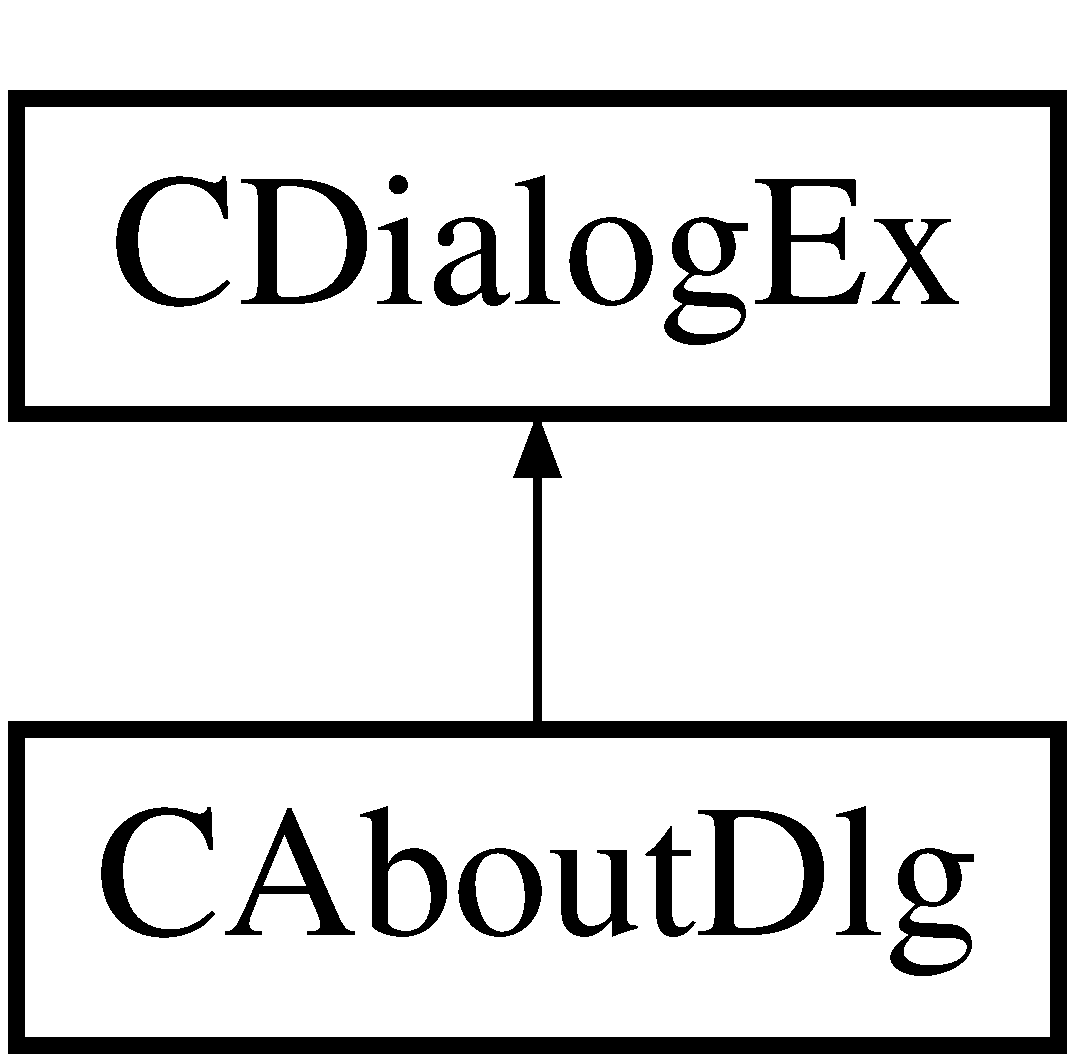
\includegraphics[height=2.000000cm]{class_c_about_dlg}
\end{center}
\end{figure}
\subsection*{Protected Member Functions}
\begin{DoxyCompactItemize}
\item 
\mbox{\Hypertarget{class_c_about_dlg_ab83db7484fec957282d7d5a21aed4df4}\label{class_c_about_dlg_ab83db7484fec957282d7d5a21aed4df4}} 
virtual void {\bfseries Do\+Data\+Exchange} (C\+Data\+Exchange $\ast$p\+DX)
\end{DoxyCompactItemize}


The documentation for this class was generated from the following file\+:\begin{DoxyCompactItemize}
\item 
Notepad/Notepad.\+cpp\end{DoxyCompactItemize}

\hypertarget{class_c_child_view}{}\section{C\+Child\+View Class Reference}
\label{class_c_child_view}\index{C\+Child\+View@{C\+Child\+View}}


子视窗类\+C\+Child\+View ~\newline
子视窗是程序中客户区部分,即文本编辑的画布部分 -\/此类继承自\+C\+Wnd  




{\ttfamily \#include $<$Child\+View.\+h$>$}

Inheritance diagram for C\+Child\+View\+:\begin{figure}[H]
\begin{center}
\leavevmode
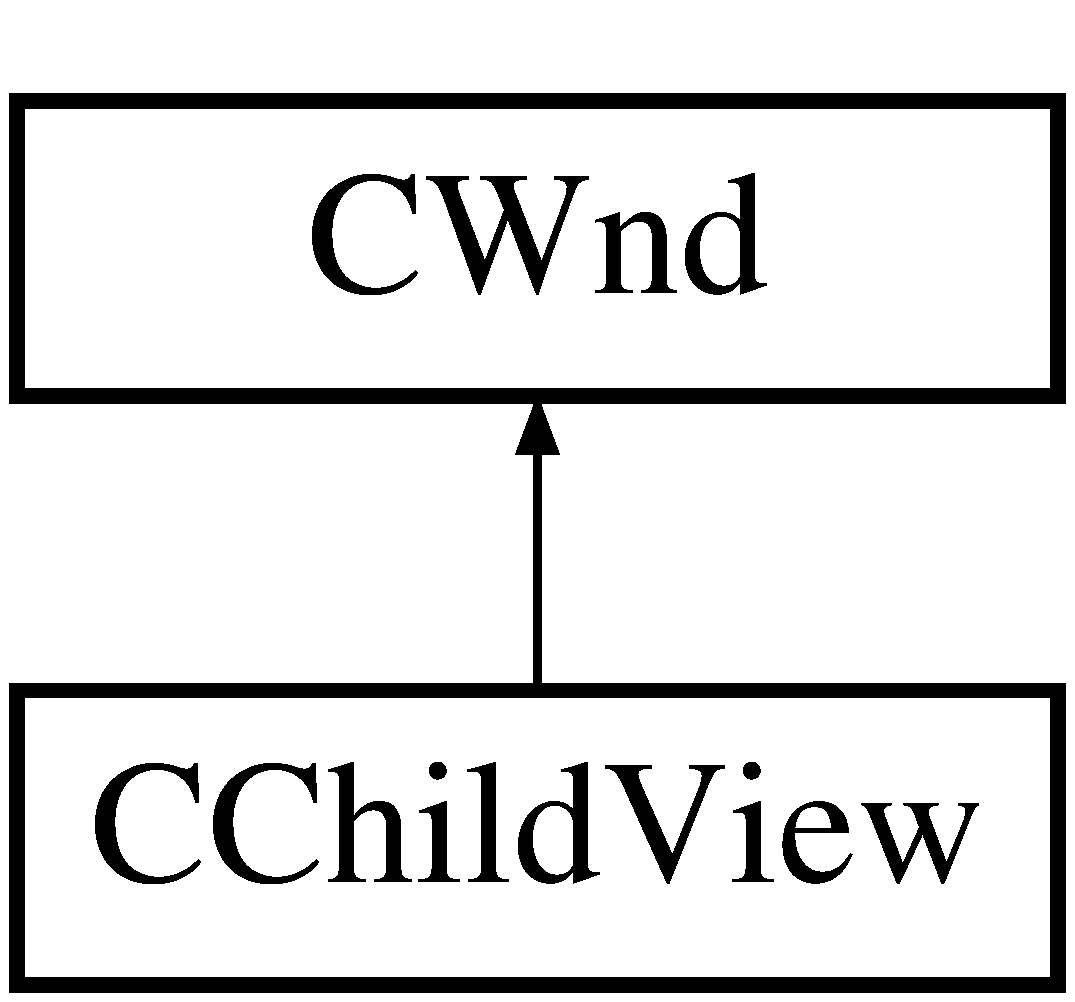
\includegraphics[height=2.000000cm]{class_c_child_view}
\end{center}
\end{figure}
\subsection*{Public Member Functions}
\begin{DoxyCompactItemize}
\item 
\mbox{\Hypertarget{class_c_child_view_aff5af7c162c10755edbe58f260ded6d4}\label{class_c_child_view_aff5af7c162c10755edbe58f260ded6d4}} 
\hyperlink{class_c_child_view_aff5af7c162c10755edbe58f260ded6d4}{C\+Child\+View} ()
\begin{DoxyCompactList}\small\item\em C\+Child\+View类构造函数 \end{DoxyCompactList}\item 
\mbox{\Hypertarget{class_c_child_view_a5b033b5e0a130950719a173b86418698}\label{class_c_child_view_a5b033b5e0a130950719a173b86418698}} 
virtual \hyperlink{class_c_child_view_a5b033b5e0a130950719a173b86418698}{$\sim$\+C\+Child\+View} ()
\begin{DoxyCompactList}\small\item\em C\+Child\+View类析构函数 \end{DoxyCompactList}\item 
void \hyperlink{class_c_child_view_a4764e41ed2ac3f2ce69916b3881894fe}{m\+\_\+paint\+Text} (C\+DC \&dc)
\begin{DoxyCompactList}\small\item\em 绘制所有文字以及背景色的函数 ~\newline
\end{DoxyCompactList}\item 
\mbox{\Hypertarget{class_c_child_view_a5acb3356732e7ea39a4468855f90fc85}\label{class_c_child_view_a5acb3356732e7ea39a4468855f90fc85}} 
void {\bfseries m\+\_\+paint\+Text} (C\+Paint\+DC \&dc)
\item 
void \hyperlink{class_c_child_view_a434383ba85ab567141366ecddeb2c9d6}{m\+\_\+paint\+Cur} (C\+DC \&dc)
\begin{DoxyCompactList}\small\item\em 绘制光标 ~\newline
\end{DoxyCompactList}\item 
\mbox{\Hypertarget{class_c_child_view_a40222a570c569017c93dd3fc088aa893}\label{class_c_child_view_a40222a570c569017c93dd3fc088aa893}} 
void {\bfseries m\+\_\+paint\+Cur} (C\+Paint\+DC \&dc)
\item 
afx\+\_\+msg void \hyperlink{class_c_child_view_af29ede94259b52b2ad54d139ff554abe}{On\+Char} (U\+I\+NT n\+Char, U\+I\+NT n\+Rep\+Cnt, U\+I\+NT n\+Flags)
\begin{DoxyCompactList}\small\item\em 响应发送文字消息的函数 ~\newline
响应\+O\+N\+\_\+\+W\+M\+\_\+\+C\+H\+A\+R消息 \end{DoxyCompactList}\item 
bool \hyperlink{class_c_child_view_a32656902f423e5c809ca20f3013fc107}{is\+\_\+input} (U\+I\+NT n\+Char)
\begin{DoxyCompactList}\small\item\em 判断是否为正常字符范围的输入 \end{DoxyCompactList}\item 
void \hyperlink{class_c_child_view_acff91e8fc8cc40cd1ebe1d24a6be4945}{m\+\_\+changed} ()
\begin{DoxyCompactList}\small\item\em 当文本内容根据用户的操作有变化的时候调用 ~\newline
操作如下~\newline
\end{DoxyCompactList}\item 
afx\+\_\+msg void \hyperlink{class_c_child_view_af513a57c45ce8b9dcc09dd934e228534}{On\+L\+Button\+Down} (U\+I\+NT n\+Flags, C\+Point point)
\begin{DoxyCompactList}\small\item\em 响应鼠标左键按下消息的函数 ~\newline
当程序收到\+O\+N\+\_\+\+W\+M\+\_\+\+L\+B\+U\+T\+T\+O\+N\+D\+O\+W\+N消息时调用该函数~\newline
主要处理两种情况~\newline

\begin{DoxyEnumerate}
\item 当没有文字被选中的时候,将光标位置调整为当前点击位置,进入选择状态
\item 没有文字被选中的时候,不作任何动作 
\end{DoxyEnumerate}\end{DoxyCompactList}\item 
afx\+\_\+msg void \hyperlink{class_c_child_view_ae81948a77ebf3744bd0f9449af57ee21}{On\+L\+Button\+Up} (U\+I\+NT n\+Flags, C\+Point point)
\begin{DoxyCompactList}\small\item\em 响应鼠标左键抬起消息的函数 ~\newline
当程序收到\+O\+N\+\_\+\+W\+M\+\_\+\+L\+B\+U\+T\+T\+O\+N\+U\+P消息时调用该函数~\newline
主要处理两种情况~\newline

\begin{DoxyEnumerate}
\item 当没有文字被选中的时候,将光标位置调整为当前抬起的位置,结束选中状态。如果鼠标左键在按下与抬起之间有移动,则会有文字被选中
\item 当有文字被选中的时候,将光标位置更新,并且取消选中状态 
\end{DoxyEnumerate}\end{DoxyCompactList}\item 
afx\+\_\+msg void \hyperlink{class_c_child_view_ad3cb2f8d9fa9a6fb06989513dee5a8bc}{On\+Mouse\+Move} (U\+I\+NT n\+Flags, C\+Point point)
\begin{DoxyCompactList}\small\item\em 响应鼠标移动消息的函数 ~\newline
当程序收到\+O\+N\+\_\+\+W\+M\+\_\+\+M\+O\+U\+S\+E\+M\+O\+V\+E消息时调用该函数~\newline
进入函数之后需要鼠标左键被按下的flag为true才会做出操作~\newline
操作主要为更新选择文字过程中的光标位置以及画面~\newline
\end{DoxyCompactList}\item 
afx\+\_\+msg void \hyperlink{class_c_child_view_a74d87512b76128e2eedea87811363e45}{On\+Key\+Down} (U\+I\+NT n\+Char, U\+I\+NT n\+Rep\+Cnt, U\+I\+NT n\+Flags)
\begin{DoxyCompactList}\small\item\em 键盘按下消息响应函数 ~\newline
此函数内部对n\+Char有判断,也就是说此函数只处理按下上下左右键的消息 \end{DoxyCompactList}\item 
afx\+\_\+msg void \hyperlink{class_c_child_view_afec062448272d8f1e15bcedcb8765abe}{On\+Key\+Up} (U\+I\+NT n\+Char, U\+I\+NT n\+Rep\+Cnt, U\+I\+NT n\+Flags)
\begin{DoxyCompactList}\small\item\em 键盘抬起消息响应函数 ~\newline
此函数内部对n\+Char有判断,也就是说此函数只处理按下上下左右键的消息 \end{DoxyCompactList}\item 
\mbox{\Hypertarget{class_c_child_view_a6060e6d09d522d345dcee5a01d41c1f0}\label{class_c_child_view_a6060e6d09d522d345dcee5a01d41c1f0}} 
afx\+\_\+msg B\+O\+OL \hyperlink{class_c_child_view_a6060e6d09d522d345dcee5a01d41c1f0}{On\+Erase\+Bkgnd} (C\+DC $\ast$p\+DC)
\begin{DoxyCompactList}\small\item\em 重载擦除屏幕函数,使它的返回值为false,即不擦除,配合双缓冲绘图使用 \end{DoxyCompactList}\item 
void \hyperlink{class_c_child_view_ab68bf2b03a8e9aab3f2aac2b9ec3177a}{curchanged} ()
\begin{DoxyCompactList}\small\item\em 重新计算页面长度以及滚动条位置 \end{DoxyCompactList}\end{DoxyCompactItemize}
\subsection*{Public Attributes}
\begin{DoxyCompactItemize}
\item 
\hyperlink{class_s_i_t_e_x_t}{S\+I\+T\+E\+XT} $\ast$ \hyperlink{class_c_child_view_a7a8d14e1c1adfb50fa6e033ebc05a357}{m\+\_\+text}
\begin{DoxyCompactList}\small\item\em 自定义的文本文字类成员 \end{DoxyCompactList}\item 
\mbox{\Hypertarget{class_c_child_view_a5c52f5e75191a707906b1334f0281376}\label{class_c_child_view_a5c52f5e75191a707906b1334f0281376}} 
\hyperlink{class_c_main_frame}{C\+Main\+Frame} $\ast$ \hyperlink{class_c_child_view_a5c52f5e75191a707906b1334f0281376}{mainframep}
\begin{DoxyCompactList}\small\item\em 指向主窗口的指针 \end{DoxyCompactList}\item 
\mbox{\Hypertarget{class_c_child_view_a7a2763ed4f49e10e4efc2c89fdf3bbbf}\label{class_c_child_view_a7a2763ed4f49e10e4efc2c89fdf3bbbf}} 
bool \hyperlink{class_c_child_view_a7a2763ed4f49e10e4efc2c89fdf3bbbf}{need\+\_\+recompute}
\begin{DoxyCompactList}\small\item\em 需要重新计算页面布局的flag \end{DoxyCompactList}\end{DoxyCompactItemize}
\subsection*{Protected Member Functions}
\begin{DoxyCompactItemize}
\item 
\mbox{\Hypertarget{class_c_child_view_a07e87a6c3606422ff10d45a47d702c7e}\label{class_c_child_view_a07e87a6c3606422ff10d45a47d702c7e}} 
virtual B\+O\+OL \hyperlink{class_c_child_view_a07e87a6c3606422ff10d45a47d702c7e}{Pre\+Create\+Window} (C\+R\+E\+A\+T\+E\+S\+T\+R\+U\+CT \&cs)
\begin{DoxyCompactList}\small\item\em 创建窗口的预处理函数 \end{DoxyCompactList}\item 
afx\+\_\+msg void \hyperlink{class_c_child_view_a8ea6d42631a4f9f446923ff864b239ab}{On\+Paint} ()
\begin{DoxyCompactList}\small\item\em 绘图函数 ~\newline
当程序接受到\+O\+N\+\_\+\+W\+M\+\_\+\+P\+A\+I\+N\+T的消息的时候就会调用该函数~\newline
该函数所做工作包括~\newline
\end{DoxyCompactList}\end{DoxyCompactItemize}


\subsection{Detailed Description}
子视窗类\+C\+Child\+View ~\newline
子视窗是程序中客户区部分,即文本编辑的画布部分 -\/此类继承自\+C\+Wnd 

\subsection{Member Function Documentation}
\mbox{\Hypertarget{class_c_child_view_ab68bf2b03a8e9aab3f2aac2b9ec3177a}\label{class_c_child_view_ab68bf2b03a8e9aab3f2aac2b9ec3177a}} 
\index{C\+Child\+View@{C\+Child\+View}!curchanged@{curchanged}}
\index{curchanged@{curchanged}!C\+Child\+View@{C\+Child\+View}}
\subsubsection{\texorpdfstring{curchanged()}{curchanged()}}
{\footnotesize\ttfamily void C\+Child\+View\+::curchanged (\begin{DoxyParamCaption}{ }\end{DoxyParamCaption})}



重新计算页面长度以及滚动条位置 

$<$adjust the=\char`\"{}\char`\"{} m\+\_\+client\+\_\+cy$>$=\char`\"{}\char`\"{}$>$

$<$/end$>$

$<$adjust the=\char`\"{}\char`\"{} screen=\char`\"{}\char`\"{} pos=\char`\"{}\char`\"{} according=\char`\"{}\char`\"{} to=\char`\"{}\char`\"{} the=\char`\"{}\char`\"{} cursor=\char`\"{}\char`\"{} pos$>$=\char`\"{}\char`\"{}$>$

$<$/end$>$ \mbox{\Hypertarget{class_c_child_view_a32656902f423e5c809ca20f3013fc107}\label{class_c_child_view_a32656902f423e5c809ca20f3013fc107}} 
\index{C\+Child\+View@{C\+Child\+View}!is\+\_\+input@{is\+\_\+input}}
\index{is\+\_\+input@{is\+\_\+input}!C\+Child\+View@{C\+Child\+View}}
\subsubsection{\texorpdfstring{is\+\_\+input()}{is\_input()}}
{\footnotesize\ttfamily bool C\+Child\+View\+::is\+\_\+input (\begin{DoxyParamCaption}\item[{U\+I\+NT}]{n\+Char }\end{DoxyParamCaption})\hspace{0.3cm}{\ttfamily [inline]}}



判断是否为正常字符范围的输入 


\begin{DoxyParams}[1]{Parameters}
\mbox{\tt in}  & {\em n\+Char} & \\
\hline
\end{DoxyParams}
\begin{DoxySeeAlso}{See also}
\hyperlink{class_c_child_view_af29ede94259b52b2ad54d139ff554abe}{On\+Char} 
\end{DoxySeeAlso}

\begin{DoxyRetVals}{Return values}
{\em true} & 是正常范围的字符 \\
\hline
{\em false} & 不是正常范围的字符 \\
\hline
\end{DoxyRetVals}
\mbox{\Hypertarget{class_c_child_view_acff91e8fc8cc40cd1ebe1d24a6be4945}\label{class_c_child_view_acff91e8fc8cc40cd1ebe1d24a6be4945}} 
\index{C\+Child\+View@{C\+Child\+View}!m\+\_\+changed@{m\+\_\+changed}}
\index{m\+\_\+changed@{m\+\_\+changed}!C\+Child\+View@{C\+Child\+View}}
\subsubsection{\texorpdfstring{m\+\_\+changed()}{m\_changed()}}
{\footnotesize\ttfamily void C\+Child\+View\+::m\+\_\+changed (\begin{DoxyParamCaption}{ }\end{DoxyParamCaption})\hspace{0.3cm}{\ttfamily [inline]}}



当文本内容根据用户的操作有变化的时候调用 ~\newline
操作如下~\newline



\begin{DoxyItemize}
\item 设置画面变化的flag(即text\+\_\+changed\+\_\+f)为true
\item 调用\+Invalidate(false)函数向程序发送重绘消息 
\end{DoxyItemize}\mbox{\Hypertarget{class_c_child_view_a434383ba85ab567141366ecddeb2c9d6}\label{class_c_child_view_a434383ba85ab567141366ecddeb2c9d6}} 
\index{C\+Child\+View@{C\+Child\+View}!m\+\_\+paint\+Cur@{m\+\_\+paint\+Cur}}
\index{m\+\_\+paint\+Cur@{m\+\_\+paint\+Cur}!C\+Child\+View@{C\+Child\+View}}
\subsubsection{\texorpdfstring{m\+\_\+paint\+Cur()}{m\_paintCur()}}
{\footnotesize\ttfamily void C\+Child\+View\+::m\+\_\+paint\+Cur (\begin{DoxyParamCaption}\item[{C\+DC \&}]{dc }\end{DoxyParamCaption})}



绘制光标 ~\newline



\begin{DoxyParams}[1]{Parameters}
\mbox{\tt in}  & {\em dc} & 当前绘图区的句柄 \\
\hline
\end{DoxyParams}
\begin{DoxyNote}{Note}
仅在\+On\+Paint函数中调用 
\end{DoxyNote}
\mbox{\Hypertarget{class_c_child_view_a4764e41ed2ac3f2ce69916b3881894fe}\label{class_c_child_view_a4764e41ed2ac3f2ce69916b3881894fe}} 
\index{C\+Child\+View@{C\+Child\+View}!m\+\_\+paint\+Text@{m\+\_\+paint\+Text}}
\index{m\+\_\+paint\+Text@{m\+\_\+paint\+Text}!C\+Child\+View@{C\+Child\+View}}
\subsubsection{\texorpdfstring{m\+\_\+paint\+Text()}{m\_paintText()}}
{\footnotesize\ttfamily void C\+Child\+View\+::m\+\_\+paint\+Text (\begin{DoxyParamCaption}\item[{C\+DC \&}]{dc }\end{DoxyParamCaption})}



绘制所有文字以及背景色的函数 ~\newline



\begin{DoxyParams}[1]{Parameters}
\mbox{\tt in}  & {\em dc} & 当前绘图区的句柄 \\
\hline
\end{DoxyParams}
\begin{DoxyNote}{Note}
仅在\+On\+Paint函数中调用 
\end{DoxyNote}
\mbox{\Hypertarget{class_c_child_view_af29ede94259b52b2ad54d139ff554abe}\label{class_c_child_view_af29ede94259b52b2ad54d139ff554abe}} 
\index{C\+Child\+View@{C\+Child\+View}!On\+Char@{On\+Char}}
\index{On\+Char@{On\+Char}!C\+Child\+View@{C\+Child\+View}}
\subsubsection{\texorpdfstring{On\+Char()}{OnChar()}}
{\footnotesize\ttfamily void C\+Child\+View\+::\+On\+Char (\begin{DoxyParamCaption}\item[{U\+I\+NT}]{n\+Char,  }\item[{U\+I\+NT}]{n\+Rep\+Cnt,  }\item[{U\+I\+NT}]{n\+Flags }\end{DoxyParamCaption})}



响应发送文字消息的函数 ~\newline
响应\+O\+N\+\_\+\+W\+M\+\_\+\+C\+H\+A\+R消息 


\begin{DoxyParams}[1]{Parameters}
\mbox{\tt in}  & {\em n\+Char} & 用户发送给系统的字符,为\+U\+I\+N\+T型,需要手动转化为wchar\+\_\+t型 \\
\hline
\mbox{\tt in}  & {\em n\+Rep\+Cnt} & 重复发送同一个消息(用户按下一个键不松手)的次数 \\
\hline
\mbox{\tt in}  & {\em n\+Flags} & 各个符号位的具体作用参见\+M\+S\+D\+N官方文档 \\
\hline
\end{DoxyParams}
\begin{DoxyNote}{Note}
请不要手动调用该函数 
\end{DoxyNote}
\mbox{\Hypertarget{class_c_child_view_a74d87512b76128e2eedea87811363e45}\label{class_c_child_view_a74d87512b76128e2eedea87811363e45}} 
\index{C\+Child\+View@{C\+Child\+View}!On\+Key\+Down@{On\+Key\+Down}}
\index{On\+Key\+Down@{On\+Key\+Down}!C\+Child\+View@{C\+Child\+View}}
\subsubsection{\texorpdfstring{On\+Key\+Down()}{OnKeyDown()}}
{\footnotesize\ttfamily void C\+Child\+View\+::\+On\+Key\+Down (\begin{DoxyParamCaption}\item[{U\+I\+NT}]{n\+Char,  }\item[{U\+I\+NT}]{n\+Rep\+Cnt,  }\item[{U\+I\+NT}]{n\+Flags }\end{DoxyParamCaption})}



键盘按下消息响应函数 ~\newline
此函数内部对n\+Char有判断,也就是说此函数只处理按下上下左右键的消息 


\begin{DoxyParams}[1]{Parameters}
\mbox{\tt in}  & {\em n\+Char} & 用户按下的键值 \\
\hline
\mbox{\tt in}  & {\em n\+Rep\+Cnt} & 用户按下该键的重复次数(用户按住该键) \\
\hline
\mbox{\tt in}  & {\em n\+Flags} & 各个符号位的具体作用参见\+M\+S\+D\+N官方文档 \\
\hline
\end{DoxyParams}
\begin{DoxyNote}{Note}
本函数只处理将光标上下左右移动的键盘消息,并且本函数只在用户按住一个键重复次数超过一的时候有效 
\end{DoxyNote}
\mbox{\Hypertarget{class_c_child_view_afec062448272d8f1e15bcedcb8765abe}\label{class_c_child_view_afec062448272d8f1e15bcedcb8765abe}} 
\index{C\+Child\+View@{C\+Child\+View}!On\+Key\+Up@{On\+Key\+Up}}
\index{On\+Key\+Up@{On\+Key\+Up}!C\+Child\+View@{C\+Child\+View}}
\subsubsection{\texorpdfstring{On\+Key\+Up()}{OnKeyUp()}}
{\footnotesize\ttfamily void C\+Child\+View\+::\+On\+Key\+Up (\begin{DoxyParamCaption}\item[{U\+I\+NT}]{n\+Char,  }\item[{U\+I\+NT}]{n\+Rep\+Cnt,  }\item[{U\+I\+NT}]{n\+Flags }\end{DoxyParamCaption})}



键盘抬起消息响应函数 ~\newline
此函数内部对n\+Char有判断,也就是说此函数只处理按下上下左右键的消息 


\begin{DoxyParams}[1]{Parameters}
\mbox{\tt in}  & {\em n\+Char} & 用户按下后抬起的键值 \\
\hline
\mbox{\tt in}  & {\em n\+Rep\+Cnt} & 用处不明 \\
\hline
\mbox{\tt in}  & {\em n\+Flags} & 各个符号位的具体作用参见\+M\+S\+D\+N官方文档 \\
\hline
\end{DoxyParams}
\begin{DoxyNote}{Note}
本函数只处理将光标上下左右移动的键盘消息 
\end{DoxyNote}
\mbox{\Hypertarget{class_c_child_view_af513a57c45ce8b9dcc09dd934e228534}\label{class_c_child_view_af513a57c45ce8b9dcc09dd934e228534}} 
\index{C\+Child\+View@{C\+Child\+View}!On\+L\+Button\+Down@{On\+L\+Button\+Down}}
\index{On\+L\+Button\+Down@{On\+L\+Button\+Down}!C\+Child\+View@{C\+Child\+View}}
\subsubsection{\texorpdfstring{On\+L\+Button\+Down()}{OnLButtonDown()}}
{\footnotesize\ttfamily void C\+Child\+View\+::\+On\+L\+Button\+Down (\begin{DoxyParamCaption}\item[{U\+I\+NT}]{n\+Flags,  }\item[{C\+Point}]{point }\end{DoxyParamCaption})}



响应鼠标左键按下消息的函数 ~\newline
当程序收到\+O\+N\+\_\+\+W\+M\+\_\+\+L\+B\+U\+T\+T\+O\+N\+D\+O\+W\+N消息时调用该函数~\newline
主要处理两种情况~\newline

\begin{DoxyEnumerate}
\item 当没有文字被选中的时候,将光标位置调整为当前点击位置,进入选择状态
\item 没有文字被选中的时候,不作任何动作 
\end{DoxyEnumerate}


\begin{DoxyParams}[1]{Parameters}
\mbox{\tt in}  & {\em n\+Flags} & 各个符号位的具体作用参见\+M\+S\+D\+N官方文档 \\
\hline
\mbox{\tt in}  & {\em point} & 返回鼠标左键按下时的屏幕坐标 \\
\hline
\end{DoxyParams}
\begin{DoxyNote}{Note}
返回的坐标值是相对于客户区左上角而言的 
\end{DoxyNote}
\mbox{\Hypertarget{class_c_child_view_ae81948a77ebf3744bd0f9449af57ee21}\label{class_c_child_view_ae81948a77ebf3744bd0f9449af57ee21}} 
\index{C\+Child\+View@{C\+Child\+View}!On\+L\+Button\+Up@{On\+L\+Button\+Up}}
\index{On\+L\+Button\+Up@{On\+L\+Button\+Up}!C\+Child\+View@{C\+Child\+View}}
\subsubsection{\texorpdfstring{On\+L\+Button\+Up()}{OnLButtonUp()}}
{\footnotesize\ttfamily void C\+Child\+View\+::\+On\+L\+Button\+Up (\begin{DoxyParamCaption}\item[{U\+I\+NT}]{n\+Flags,  }\item[{C\+Point}]{point }\end{DoxyParamCaption})}



响应鼠标左键抬起消息的函数 ~\newline
当程序收到\+O\+N\+\_\+\+W\+M\+\_\+\+L\+B\+U\+T\+T\+O\+N\+U\+P消息时调用该函数~\newline
主要处理两种情况~\newline

\begin{DoxyEnumerate}
\item 当没有文字被选中的时候,将光标位置调整为当前抬起的位置,结束选中状态。如果鼠标左键在按下与抬起之间有移动,则会有文字被选中
\item 当有文字被选中的时候,将光标位置更新,并且取消选中状态 
\end{DoxyEnumerate}


\begin{DoxyParams}[1]{Parameters}
\mbox{\tt in}  & {\em n\+Flags} & 各个符号位的具体作用参见\+M\+S\+D\+N官方文档 \\
\hline
\mbox{\tt in}  & {\em point} & 返回鼠标左键抬起时的屏幕坐标 \\
\hline
\end{DoxyParams}
\begin{DoxyNote}{Note}
返回的坐标值是相对于客户区左上角而言的 
\end{DoxyNote}
\mbox{\Hypertarget{class_c_child_view_ad3cb2f8d9fa9a6fb06989513dee5a8bc}\label{class_c_child_view_ad3cb2f8d9fa9a6fb06989513dee5a8bc}} 
\index{C\+Child\+View@{C\+Child\+View}!On\+Mouse\+Move@{On\+Mouse\+Move}}
\index{On\+Mouse\+Move@{On\+Mouse\+Move}!C\+Child\+View@{C\+Child\+View}}
\subsubsection{\texorpdfstring{On\+Mouse\+Move()}{OnMouseMove()}}
{\footnotesize\ttfamily void C\+Child\+View\+::\+On\+Mouse\+Move (\begin{DoxyParamCaption}\item[{U\+I\+NT}]{n\+Flags,  }\item[{C\+Point}]{point }\end{DoxyParamCaption})}



响应鼠标移动消息的函数 ~\newline
当程序收到\+O\+N\+\_\+\+W\+M\+\_\+\+M\+O\+U\+S\+E\+M\+O\+V\+E消息时调用该函数~\newline
进入函数之后需要鼠标左键被按下的flag为true才会做出操作~\newline
操作主要为更新选择文字过程中的光标位置以及画面~\newline



\begin{DoxyParams}[1]{Parameters}
\mbox{\tt in}  & {\em n\+Flags} & 各个符号位的具体作用参见\+M\+S\+D\+N官方文档 \\
\hline
\mbox{\tt in}  & {\em point} & 返回鼠标移动时的屏幕坐标 \\
\hline
\end{DoxyParams}
\begin{DoxyNote}{Note}
返回的坐标值是相对于客户区左上角而言的 
\end{DoxyNote}
\mbox{\Hypertarget{class_c_child_view_a8ea6d42631a4f9f446923ff864b239ab}\label{class_c_child_view_a8ea6d42631a4f9f446923ff864b239ab}} 
\index{C\+Child\+View@{C\+Child\+View}!On\+Paint@{On\+Paint}}
\index{On\+Paint@{On\+Paint}!C\+Child\+View@{C\+Child\+View}}
\subsubsection{\texorpdfstring{On\+Paint()}{OnPaint()}}
{\footnotesize\ttfamily void C\+Child\+View\+::\+On\+Paint (\begin{DoxyParamCaption}{ }\end{DoxyParamCaption})\hspace{0.3cm}{\ttfamily [protected]}}



绘图函数 ~\newline
当程序接受到\+O\+N\+\_\+\+W\+M\+\_\+\+P\+A\+I\+N\+T的消息的时候就会调用该函数~\newline
该函数所做工作包括~\newline



\begin{DoxyItemize}
\item 重新计算所有文字的位置
\item 重新绘制画面,包括所有文字以及背景色
\item 将需要重绘的flag(即text\+\_\+changed\+\_\+f)置为flase \begin{DoxyNote}{Note}
请不要手动调用该函数,如需重绘画面请用\+Invalidate(false);函数 
\end{DoxyNote}

\end{DoxyItemize}

\subsection{Member Data Documentation}
\mbox{\Hypertarget{class_c_child_view_a7a8d14e1c1adfb50fa6e033ebc05a357}\label{class_c_child_view_a7a8d14e1c1adfb50fa6e033ebc05a357}} 
\index{C\+Child\+View@{C\+Child\+View}!m\+\_\+text@{m\+\_\+text}}
\index{m\+\_\+text@{m\+\_\+text}!C\+Child\+View@{C\+Child\+View}}
\subsubsection{\texorpdfstring{m\+\_\+text}{m\_text}}
{\footnotesize\ttfamily \hyperlink{class_s_i_t_e_x_t}{S\+I\+T\+E\+XT}$\ast$ C\+Child\+View\+::m\+\_\+text}



自定义的文本文字类成员 

\begin{DoxySeeAlso}{See also}
class \hyperlink{class_s_i_t_e_x_t}{S\+I\+T\+E\+XT} 
\end{DoxySeeAlso}


The documentation for this class was generated from the following files\+:\begin{DoxyCompactItemize}
\item 
Notepad/\hyperlink{_child_view_8h}{Child\+View.\+h}\item 
Notepad/Child\+View.\+cpp\end{DoxyCompactItemize}

\hypertarget{class_c_main_frame}{}\section{C\+Main\+Frame类 参考}
\label{class_c_main_frame}\index{C\+Main\+Frame@{C\+Main\+Frame}}


程序主框架类\+C\+Main\+Frame类 ~\newline
主框架包括子视图类以及滚动条 继承自\+C\+Frame\+Wnd类  




{\ttfamily \#include $<$Main\+Frm.\+h$>$}

类 C\+Main\+Frame 继承关系图\+:\begin{figure}[H]
\begin{center}
\leavevmode
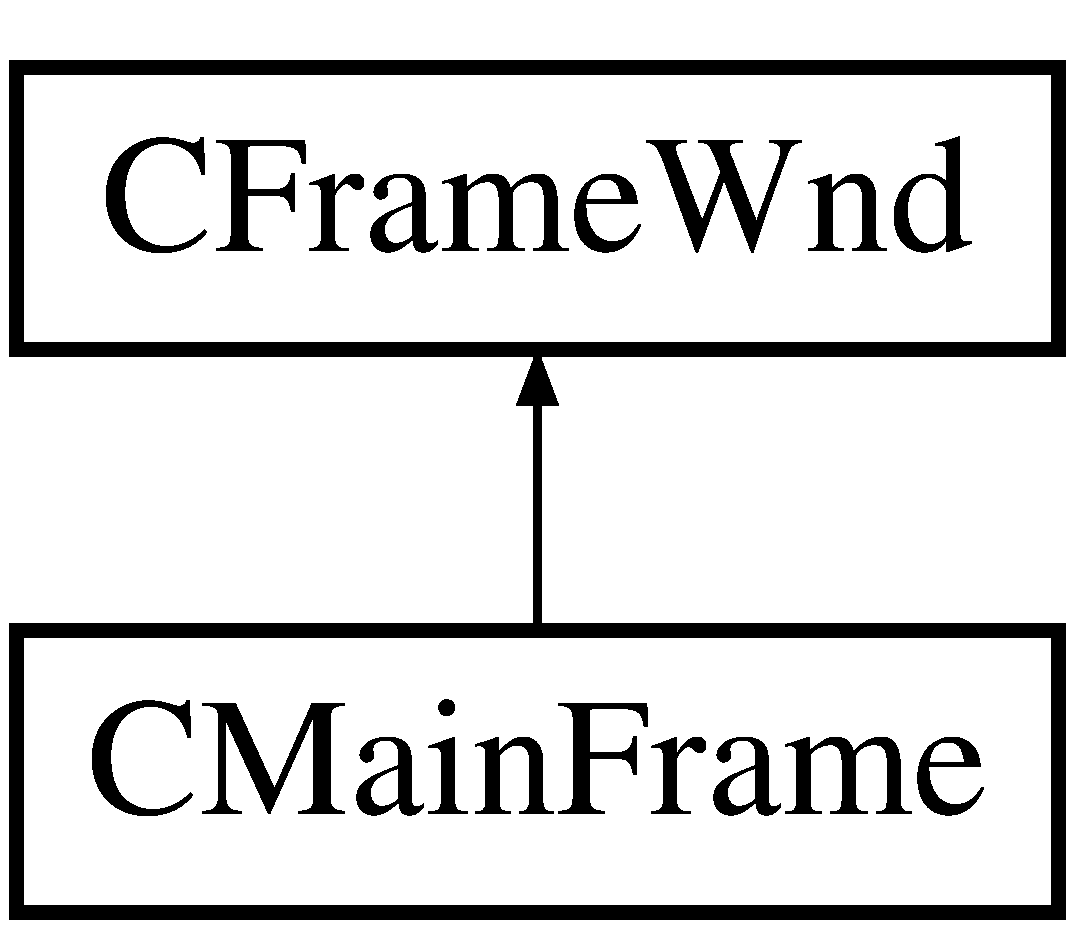
\includegraphics[height=2.000000cm]{class_c_main_frame}
\end{center}
\end{figure}
\subsection*{Public 成员函数}
\begin{DoxyCompactItemize}
\item 
\hyperlink{class_c_main_frame_af3e997aeae4148d2aaa4a1e1ae7bdd53}{C\+Main\+Frame} ()
\begin{DoxyCompactList}\small\item\em C\+Main\+Frame类构造函数~\newline
初始化部分成员变量 \end{DoxyCompactList}\item 
\mbox{\Hypertarget{class_c_main_frame_a549bf677c955c2898c3c683321633c16}\label{class_c_main_frame_a549bf677c955c2898c3c683321633c16}} 
virtual B\+O\+OL \hyperlink{class_c_main_frame_a549bf677c955c2898c3c683321633c16}{Pre\+Create\+Window} (C\+R\+E\+A\+T\+E\+S\+T\+R\+U\+CT \&cs)
\begin{DoxyCompactList}\small\item\em 绘图预处理函数,如果需要修改窗口样式则改写该函数 \end{DoxyCompactList}\item 
\mbox{\Hypertarget{class_c_main_frame_ade959eb0bab719bf06bb9b18ee407101}\label{class_c_main_frame_ade959eb0bab719bf06bb9b18ee407101}} 
virtual B\+O\+OL \hyperlink{class_c_main_frame_ade959eb0bab719bf06bb9b18ee407101}{On\+Cmd\+Msg} (U\+I\+NT n\+ID, int n\+Code, void $\ast$p\+Extra, A\+F\+X\+\_\+\+C\+M\+D\+H\+A\+N\+D\+L\+E\+R\+I\+N\+FO $\ast$p\+Handler\+Info)
\begin{DoxyCompactList}\small\item\em 主消息循环函数,无需修改 \end{DoxyCompactList}\item 
\mbox{\Hypertarget{class_c_main_frame_a8ae555f23fdf97edb4feb4d3e1bfa4ee}\label{class_c_main_frame_a8ae555f23fdf97edb4feb4d3e1bfa4ee}} 
virtual \hyperlink{class_c_main_frame_a8ae555f23fdf97edb4feb4d3e1bfa4ee}{$\sim$\+C\+Main\+Frame} ()
\begin{DoxyCompactList}\small\item\em 默认析构函数 \end{DoxyCompactList}\item 
void \hyperlink{class_c_main_frame_a2500e3a6ace77e01430f5ff4b9a6f182}{Update\+Client\+Rect} ()
\begin{DoxyCompactList}\small\item\em 当窗口大小被调整之后调用的函数~\newline
\end{DoxyCompactList}\item 
afx\+\_\+msg void \hyperlink{class_c_main_frame_adf171bf1f2c6f10cc85dbe8db3fc93f7}{On\+Size} (U\+I\+NT n\+Type, int cx, int cy)
\begin{DoxyCompactList}\small\item\em 当窗口大小被调整之后调用的消息响应函数~\newline
当窗口大小被调整,共有两个地方需要调整~\newline
\end{DoxyCompactList}\item 
afx\+\_\+msg void \hyperlink{class_c_main_frame_a969c7e78dee0c54e7bcbe2ab9c901cc2}{On\+V\+Scroll} (U\+I\+NT n\+S\+B\+Code, U\+I\+NT n\+Pos, C\+Scroll\+Bar $\ast$p\+Scroll\+Bar)
\begin{DoxyCompactList}\small\item\em 改变滚动块的位置时调用的函数~\newline
调整两个地方~\newline
\end{DoxyCompactList}\item 
void \hyperlink{class_c_main_frame_a4f7c9f6d9aeae93045c5dd2047ccebf1}{Update\+Scroll\+Bar\+Pos} ()
\begin{DoxyCompactList}\small\item\em 当改变窗口大小时,调整滚动块的位置~\newline
通过记录页面相对于上边界的偏移量来调整 \end{DoxyCompactList}\end{DoxyCompactItemize}
\subsection*{Public 属性}
\begin{DoxyCompactItemize}
\item 
\mbox{\Hypertarget{class_c_main_frame_a7c3af9327c496f8c807d578f7a4ef4c5}\label{class_c_main_frame_a7c3af9327c496f8c807d578f7a4ef4c5}} 
\hyperlink{class_c_child_view}{C\+Child\+View} \hyperlink{class_c_main_frame_a7c3af9327c496f8c807d578f7a4ef4c5}{m\+\_\+wnd\+View}
\begin{DoxyCompactList}\small\item\em 子视图类成员变量 \end{DoxyCompactList}\item 
\mbox{\Hypertarget{class_c_main_frame_a0c53b2f10889123e0c4cf8912816aeaf}\label{class_c_main_frame_a0c53b2f10889123e0c4cf8912816aeaf}} 
C\+Rect \hyperlink{class_c_main_frame_a0c53b2f10889123e0c4cf8912816aeaf}{m\+\_\+client\+\_\+rect}
\begin{DoxyCompactList}\small\item\em 用于存储客户区的大小的变量 \end{DoxyCompactList}\item 
\mbox{\Hypertarget{class_c_main_frame_ad561552de446751652ae4e98ded06589}\label{class_c_main_frame_ad561552de446751652ae4e98ded06589}} 
int \hyperlink{class_c_main_frame_ad561552de446751652ae4e98ded06589}{m\+\_\+client\+\_\+cy}
\begin{DoxyCompactList}\small\item\em 用于存储子视图的y方向的长度 \end{DoxyCompactList}\item 
\mbox{\Hypertarget{class_c_main_frame_a342befca89935d78753d6a78514b83c5}\label{class_c_main_frame_a342befca89935d78753d6a78514b83c5}} 
int \hyperlink{class_c_main_frame_a342befca89935d78753d6a78514b83c5}{scrolledpix}
\begin{DoxyCompactList}\small\item\em 用于记录页面相对于上边界偏移量 \end{DoxyCompactList}\item 
\mbox{\Hypertarget{class_c_main_frame_a94f2543f4d46fdb15202c5386ef4ee0a}\label{class_c_main_frame_a94f2543f4d46fdb15202c5386ef4ee0a}} 
int \hyperlink{class_c_main_frame_a94f2543f4d46fdb15202c5386ef4ee0a}{maincx}
\begin{DoxyCompactList}\small\item\em 记录当前客户区的宽度 \end{DoxyCompactList}\item 
\mbox{\Hypertarget{class_c_main_frame_abfc6b521bf0730404603a66171e51159}\label{class_c_main_frame_abfc6b521bf0730404603a66171e51159}} 
int \hyperlink{class_c_main_frame_abfc6b521bf0730404603a66171e51159}{maincy}
\begin{DoxyCompactList}\small\item\em 记录当前客户区的高度 \end{DoxyCompactList}\end{DoxyCompactItemize}
\subsection*{Protected 成员函数}
\begin{DoxyCompactItemize}
\item 
afx\+\_\+msg int \hyperlink{class_c_main_frame_a48666466fd37412fcaeff75c3b12e0ed}{On\+Create} (L\+P\+C\+R\+E\+A\+T\+E\+S\+T\+R\+U\+CT lp\+Create\+Struct)
\begin{DoxyCompactList}\small\item\em 创建主窗口时调用的函数~\newline
创建了两个实例~\newline
\end{DoxyCompactList}\item 
\mbox{\Hypertarget{class_c_main_frame_adc353a3d1fc497fbc009b6d9e6914a82}\label{class_c_main_frame_adc353a3d1fc497fbc009b6d9e6914a82}} 
afx\+\_\+msg void \hyperlink{class_c_main_frame_adc353a3d1fc497fbc009b6d9e6914a82}{On\+Set\+Focus} (C\+Wnd $\ast$p\+Old\+Wnd)
\begin{DoxyCompactList}\small\item\em 当窗口被聚焦的时候调用,无需修改 \end{DoxyCompactList}\end{DoxyCompactItemize}
\subsection*{Protected 属性}
\begin{DoxyCompactItemize}
\item 
\mbox{\Hypertarget{class_c_main_frame_afa369311a084e7ff2af17a819829b21b}\label{class_c_main_frame_afa369311a084e7ff2af17a819829b21b}} 
C\+Scroll\+Bar \hyperlink{class_c_main_frame_afa369311a084e7ff2af17a819829b21b}{m\+\_\+scroll\+Bar}
\begin{DoxyCompactList}\small\item\em 滚动条类成员 \end{DoxyCompactList}\end{DoxyCompactItemize}


\subsection{详细描述}
程序主框架类\+C\+Main\+Frame类 ~\newline
主框架包括子视图类以及滚动条 继承自\+C\+Frame\+Wnd类 

\subsection{构造及析构函数说明}
\mbox{\Hypertarget{class_c_main_frame_af3e997aeae4148d2aaa4a1e1ae7bdd53}\label{class_c_main_frame_af3e997aeae4148d2aaa4a1e1ae7bdd53}} 
\index{C\+Main\+Frame@{C\+Main\+Frame}!C\+Main\+Frame@{C\+Main\+Frame}}
\index{C\+Main\+Frame@{C\+Main\+Frame}!C\+Main\+Frame@{C\+Main\+Frame}}
\subsubsection{\texorpdfstring{C\+Main\+Frame()}{CMainFrame()}}
{\footnotesize\ttfamily C\+Main\+Frame\+::\+C\+Main\+Frame (\begin{DoxyParamCaption}{ }\end{DoxyParamCaption})}



C\+Main\+Frame类构造函数~\newline
初始化部分成员变量 


\begin{DoxyItemize}
\item m\+\_\+client\+\_\+cy = 10000
\item scrolledpix = 0 
\end{DoxyItemize}

\subsection{成员函数说明}
\mbox{\Hypertarget{class_c_main_frame_a48666466fd37412fcaeff75c3b12e0ed}\label{class_c_main_frame_a48666466fd37412fcaeff75c3b12e0ed}} 
\index{C\+Main\+Frame@{C\+Main\+Frame}!On\+Create@{On\+Create}}
\index{On\+Create@{On\+Create}!C\+Main\+Frame@{C\+Main\+Frame}}
\subsubsection{\texorpdfstring{On\+Create()}{OnCreate()}}
{\footnotesize\ttfamily int C\+Main\+Frame\+::\+On\+Create (\begin{DoxyParamCaption}\item[{L\+P\+C\+R\+E\+A\+T\+E\+S\+T\+R\+U\+CT}]{lp\+Create\+Struct }\end{DoxyParamCaption})\hspace{0.3cm}{\ttfamily [protected]}}



创建主窗口时调用的函数~\newline
创建了两个实例~\newline



\begin{DoxyItemize}
\item \hyperlink{class_c_child_view}{C\+Child\+View} m\+\_\+wnd\+View \begin{DoxySeeAlso}{参见}
\hyperlink{class_c_child_view}{C\+Child\+View}
\end{DoxySeeAlso}

\item C\+Scroll\+Bar m\+\_\+scroll\+Bar 竖直滚动条实例 
\begin{DoxyParams}[1]{参数}
\mbox{\tt in}  & {\em lp\+Create\+Struct} & 至于这个是什么不重要,不需要自己调用这个函数 \\
\hline
\end{DoxyParams}

\end{DoxyItemize}\mbox{\Hypertarget{class_c_main_frame_adf171bf1f2c6f10cc85dbe8db3fc93f7}\label{class_c_main_frame_adf171bf1f2c6f10cc85dbe8db3fc93f7}} 
\index{C\+Main\+Frame@{C\+Main\+Frame}!On\+Size@{On\+Size}}
\index{On\+Size@{On\+Size}!C\+Main\+Frame@{C\+Main\+Frame}}
\subsubsection{\texorpdfstring{On\+Size()}{OnSize()}}
{\footnotesize\ttfamily void C\+Main\+Frame\+::\+On\+Size (\begin{DoxyParamCaption}\item[{U\+I\+NT}]{n\+Type,  }\item[{int}]{cx,  }\item[{int}]{cy }\end{DoxyParamCaption})}



当窗口大小被调整之后调用的消息响应函数~\newline
当窗口大小被调整,共有两个地方需要调整~\newline



\begin{DoxyItemize}
\item 子窗口的大小~\newline
通过调用\+Update\+Client\+Rect函数 \begin{DoxySeeAlso}{参见}
\hyperlink{class_c_main_frame_a2500e3a6ace77e01430f5ff4b9a6f182}{Update\+Client\+Rect}
\end{DoxySeeAlso}

\item 滚动条的一系列调整~\newline
 滚动条的长度调整~\newline
 滚动条上拖动块的位置调整 
\begin{DoxyParams}[1]{参数}
\mbox{\tt in}  & {\em n\+Type} & 参阅\+M\+S\+D\+N官方文档 \\
\hline
\mbox{\tt in}  & {\em cx} & 由系统传入当前窗口x方向的长度 \\
\hline
\mbox{\tt in}  & {\em cy} & 有系统传入当前窗口y方向的长度 \\
\hline
\end{DoxyParams}
\begin{DoxyNote}{注解}
无需自己调用,当手动改变窗口大小的时候,系统会传入\+O\+N\+\_\+\+W\+M\+\_\+\+S\+I\+Z\+E消息,此时会自动调用该函数 
\end{DoxyNote}

\end{DoxyItemize}\mbox{\Hypertarget{class_c_main_frame_a969c7e78dee0c54e7bcbe2ab9c901cc2}\label{class_c_main_frame_a969c7e78dee0c54e7bcbe2ab9c901cc2}} 
\index{C\+Main\+Frame@{C\+Main\+Frame}!On\+V\+Scroll@{On\+V\+Scroll}}
\index{On\+V\+Scroll@{On\+V\+Scroll}!C\+Main\+Frame@{C\+Main\+Frame}}
\subsubsection{\texorpdfstring{On\+V\+Scroll()}{OnVScroll()}}
{\footnotesize\ttfamily void C\+Main\+Frame\+::\+On\+V\+Scroll (\begin{DoxyParamCaption}\item[{U\+I\+NT}]{n\+S\+B\+Code,  }\item[{U\+I\+NT}]{n\+Pos,  }\item[{C\+Scroll\+Bar $\ast$}]{p\+Scroll\+Bar }\end{DoxyParamCaption})}



改变滚动块的位置时调用的函数~\newline
调整两个地方~\newline



\begin{DoxyItemize}
\item 子视图的位置
\item 滚动块的位置更新 
\begin{DoxyParams}[1]{参数}
\mbox{\tt in}  & {\em n\+S\+B\+Code} & 参阅\+M\+S\+D\+N官方文档 \\
\hline
\mbox{\tt in}  & {\em n\+Pos} & 参阅\+M\+S\+D\+N官方文档 \\
\hline
\mbox{\tt in}  & {\em p\+Scroll\+Bar} & 当前被滑动的滚动条的指针 \\
\hline
\end{DoxyParams}

\end{DoxyItemize}\mbox{\Hypertarget{class_c_main_frame_a2500e3a6ace77e01430f5ff4b9a6f182}\label{class_c_main_frame_a2500e3a6ace77e01430f5ff4b9a6f182}} 
\index{C\+Main\+Frame@{C\+Main\+Frame}!Update\+Client\+Rect@{Update\+Client\+Rect}}
\index{Update\+Client\+Rect@{Update\+Client\+Rect}!C\+Main\+Frame@{C\+Main\+Frame}}
\subsubsection{\texorpdfstring{Update\+Client\+Rect()}{UpdateClientRect()}}
{\footnotesize\ttfamily void C\+Main\+Frame\+::\+Update\+Client\+Rect (\begin{DoxyParamCaption}{ }\end{DoxyParamCaption})}



当窗口大小被调整之后调用的函数~\newline



\begin{DoxyParams}[1]{参数}
\mbox{\tt in}  & {\em cx} & 当前窗口x方向长度 \\
\hline
\mbox{\tt in}  & {\em cy} & 当前窗口y方向长度 \\
\hline
\end{DoxyParams}
\begin{DoxyNote}{注解}
该函数仅在\+On\+Size函数中被调用,因为传入的参数需要用到\+On\+Size函数的传入值 
\end{DoxyNote}
\begin{DoxySeeAlso}{参见}
\hyperlink{class_c_main_frame_adf171bf1f2c6f10cc85dbe8db3fc93f7}{On\+Size} 
\end{DoxySeeAlso}
\mbox{\Hypertarget{class_c_main_frame_a4f7c9f6d9aeae93045c5dd2047ccebf1}\label{class_c_main_frame_a4f7c9f6d9aeae93045c5dd2047ccebf1}} 
\index{C\+Main\+Frame@{C\+Main\+Frame}!Update\+Scroll\+Bar\+Pos@{Update\+Scroll\+Bar\+Pos}}
\index{Update\+Scroll\+Bar\+Pos@{Update\+Scroll\+Bar\+Pos}!C\+Main\+Frame@{C\+Main\+Frame}}
\subsubsection{\texorpdfstring{Update\+Scroll\+Bar\+Pos()}{UpdateScrollBarPos()}}
{\footnotesize\ttfamily void C\+Main\+Frame\+::\+Update\+Scroll\+Bar\+Pos (\begin{DoxyParamCaption}{ }\end{DoxyParamCaption})}



当改变窗口大小时,调整滚动块的位置~\newline
通过记录页面相对于上边界的偏移量来调整 

\begin{DoxyNote}{注解}
此函数仅在\+On\+Size函数中调用 
\end{DoxyNote}
\begin{DoxySeeAlso}{参见}
On\+Size重置滚动条位置 
\end{DoxySeeAlso}


该类的文档由以下文件生成\+:\begin{DoxyCompactItemize}
\item 
Notepad/\hyperlink{_main_frm_8h}{Main\+Frm.\+h}\item 
Notepad/Main\+Frm.\+cpp\end{DoxyCompactItemize}

\hypertarget{class_c_notepad_app}{}\section{C\+Notepad\+App类 参考}
\label{class_c_notepad_app}\index{C\+Notepad\+App@{C\+Notepad\+App}}


程序大类\+C\+Notepad\+App~\newline
程序启动时创建,初始化函数中创建其他的对象~\newline
在初始化过程中创建菜单,主窗口~\newline
继承自\+C\+Win\+App  




{\ttfamily \#include $<$Notepad.\+h$>$}

类 C\+Notepad\+App 继承关系图\+:\begin{figure}[H]
\begin{center}
\leavevmode
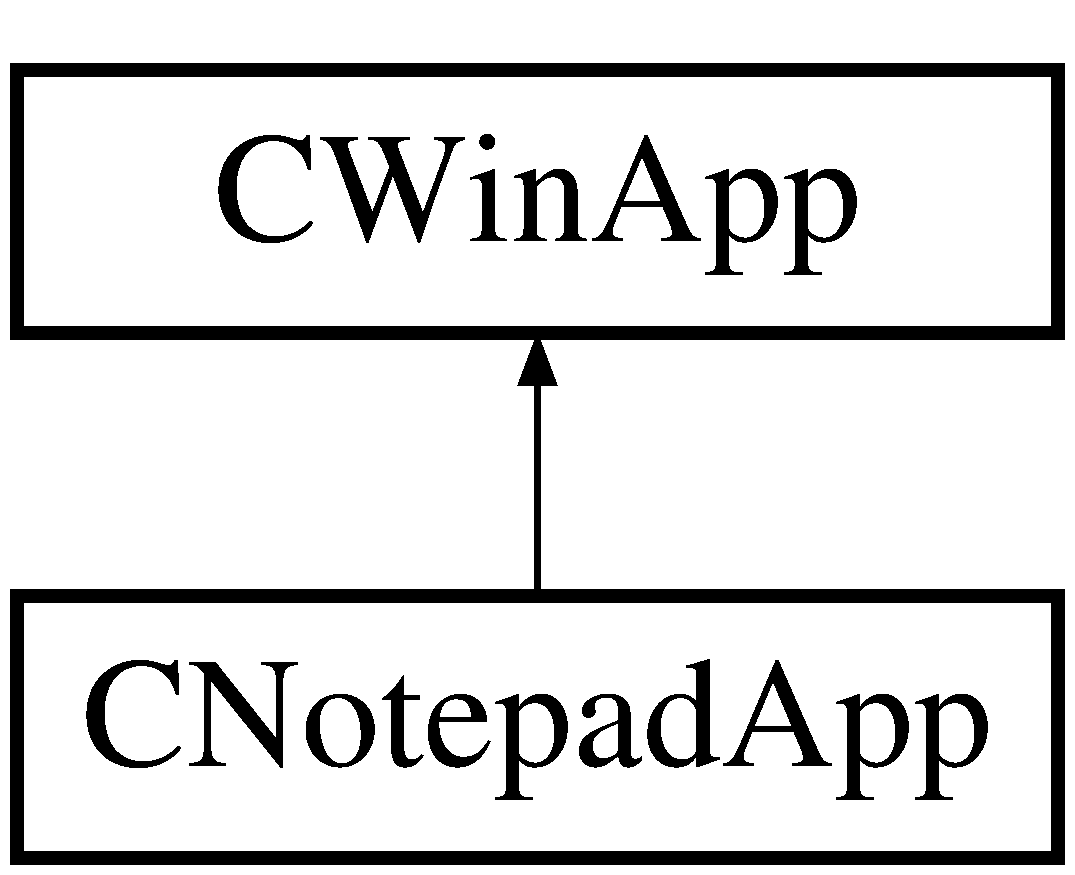
\includegraphics[height=2.000000cm]{class_c_notepad_app}
\end{center}
\end{figure}
\subsection*{Public 成员函数}
\begin{DoxyCompactItemize}
\item 
\mbox{\Hypertarget{class_c_notepad_app_a829ed77997eb81496b815b50657ecb40}\label{class_c_notepad_app_a829ed77997eb81496b815b50657ecb40}} 
\hyperlink{class_c_notepad_app_a829ed77997eb81496b815b50657ecb40}{C\+Notepad\+App} ()
\begin{DoxyCompactList}\small\item\em 默认构造函数 \end{DoxyCompactList}\item 
\mbox{\Hypertarget{class_c_notepad_app_a31874d4fcf2e5120379146e61d8716d4}\label{class_c_notepad_app_a31874d4fcf2e5120379146e61d8716d4}} 
virtual B\+O\+OL \hyperlink{class_c_notepad_app_a31874d4fcf2e5120379146e61d8716d4}{Init\+Instance} ()
\begin{DoxyCompactList}\small\item\em 初始化函数,实例化\+C\+Main\+Frame类,并且将mainp指针指向它 \end{DoxyCompactList}\item 
\mbox{\Hypertarget{class_c_notepad_app_a07647790b646bc0be54fbf39e069ddcd}\label{class_c_notepad_app_a07647790b646bc0be54fbf39e069ddcd}} 
virtual int \hyperlink{class_c_notepad_app_a07647790b646bc0be54fbf39e069ddcd}{Exit\+Instance} ()
\begin{DoxyCompactList}\small\item\em 退出程序调用函数 \end{DoxyCompactList}\item 
afx\+\_\+msg void \hyperlink{class_c_notepad_app_aa09334de95a65c56cdca8a682b006bb6}{On\+Font} ()
\begin{DoxyCompactList}\small\item\em 选择字体消息响应函数~\newline
\end{DoxyCompactList}\item 
afx\+\_\+msg void \hyperlink{class_c_notepad_app_a954649ecbb87fb8a001f2ed399440261}{On\+Para} ()
\begin{DoxyCompactList}\small\item\em 选择行间距字间距消息响应函数~\newline
\end{DoxyCompactList}\item 
\mbox{\Hypertarget{class_c_notepad_app_a66c1b4a1e235017e0a5078438df97e7c}\label{class_c_notepad_app_a66c1b4a1e235017e0a5078438df97e7c}} 
afx\+\_\+msg void {\bfseries On\+Cut} ()
\item 
\mbox{\Hypertarget{class_c_notepad_app_aa3444dcefa48928a6244b98d337cbff9}\label{class_c_notepad_app_aa3444dcefa48928a6244b98d337cbff9}} 
afx\+\_\+msg void {\bfseries On\+Copy} ()
\item 
\mbox{\Hypertarget{class_c_notepad_app_af6bb7c7de2fcddd4245c5005135c1689}\label{class_c_notepad_app_af6bb7c7de2fcddd4245c5005135c1689}} 
afx\+\_\+msg void {\bfseries On\+Paste} ()
\item 
\mbox{\Hypertarget{class_c_notepad_app_a40ce59e5a4884458f47b49b80497683a}\label{class_c_notepad_app_a40ce59e5a4884458f47b49b80497683a}} 
afx\+\_\+msg void \hyperlink{class_c_notepad_app_a40ce59e5a4884458f47b49b80497683a}{On\+App\+About} ()
\begin{DoxyCompactList}\small\item\em \char`\"{}关于\char`\"{}窗口的消息相应函数 \end{DoxyCompactList}\item 
\mbox{\Hypertarget{class_c_notepad_app_add137cbf475cc2218fcaa715b22c283b}\label{class_c_notepad_app_add137cbf475cc2218fcaa715b22c283b}} 
afx\+\_\+msg void \hyperlink{class_c_notepad_app_add137cbf475cc2218fcaa715b22c283b}{On\+Align\+Left} ()
\begin{DoxyCompactList}\small\item\em 左对齐的消息响应函数 \end{DoxyCompactList}\item 
\mbox{\Hypertarget{class_c_notepad_app_abc249a300c4b6f43bead2d500831fe35}\label{class_c_notepad_app_abc249a300c4b6f43bead2d500831fe35}} 
afx\+\_\+msg void \hyperlink{class_c_notepad_app_abc249a300c4b6f43bead2d500831fe35}{On\+Align\+Center} ()
\begin{DoxyCompactList}\small\item\em 居中的消息响应函数农户 \end{DoxyCompactList}\item 
\mbox{\Hypertarget{class_c_notepad_app_ac89fe310647cf5fbc03538346cbc4c10}\label{class_c_notepad_app_ac89fe310647cf5fbc03538346cbc4c10}} 
afx\+\_\+msg void \hyperlink{class_c_notepad_app_ac89fe310647cf5fbc03538346cbc4c10}{On\+Align\+Right} ()
\begin{DoxyCompactList}\small\item\em 右对齐的消息响应函数 \end{DoxyCompactList}\item 
\mbox{\Hypertarget{class_c_notepad_app_abbcfd489cd0440ed1551fe41396f6cdd}\label{class_c_notepad_app_abbcfd489cd0440ed1551fe41396f6cdd}} 
afx\+\_\+msg void \hyperlink{class_c_notepad_app_abbcfd489cd0440ed1551fe41396f6cdd}{On\+Align\+Distribute} ()
\begin{DoxyCompactList}\small\item\em 分散对齐的消息响应函数 \end{DoxyCompactList}\item 
\mbox{\Hypertarget{class_c_notepad_app_afcebb68584ad362f5dfba2449194531d}\label{class_c_notepad_app_afcebb68584ad362f5dfba2449194531d}} 
afx\+\_\+msg void \hyperlink{class_c_notepad_app_afcebb68584ad362f5dfba2449194531d}{On\+Open} ()
\begin{DoxyCompactList}\small\item\em 打开文件的消息响应函数 \end{DoxyCompactList}\item 
\mbox{\Hypertarget{class_c_notepad_app_a9fcc45c39d4fb4866c0b7f2e1f1b27c0}\label{class_c_notepad_app_a9fcc45c39d4fb4866c0b7f2e1f1b27c0}} 
afx\+\_\+msg void \hyperlink{class_c_notepad_app_a9fcc45c39d4fb4866c0b7f2e1f1b27c0}{On\+Close} ()
\begin{DoxyCompactList}\small\item\em 关闭文件的消息响应函数 \end{DoxyCompactList}\item 
\mbox{\Hypertarget{class_c_notepad_app_aedb9f07cbb0e5ef12c51f6e829c3a1bf}\label{class_c_notepad_app_aedb9f07cbb0e5ef12c51f6e829c3a1bf}} 
void \hyperlink{class_c_notepad_app_aedb9f07cbb0e5ef12c51f6e829c3a1bf}{change\+\_\+align} (int flag)
\begin{DoxyCompactList}\small\item\em 改变对齐方式的函数 \end{DoxyCompactList}\end{DoxyCompactItemize}
\subsection*{Public 属性}
\begin{DoxyCompactItemize}
\item 
\mbox{\Hypertarget{class_c_notepad_app_a9eee0a246d98c97f2554d5bd292bf3f1}\label{class_c_notepad_app_a9eee0a246d98c97f2554d5bd292bf3f1}} 
\hyperlink{class_c_main_frame}{C\+Main\+Frame} $\ast$ \hyperlink{class_c_notepad_app_a9eee0a246d98c97f2554d5bd292bf3f1}{mainp}
\begin{DoxyCompactList}\small\item\em 指向主窗口的指针 \end{DoxyCompactList}\item 
\mbox{\Hypertarget{class_c_notepad_app_a7659b246dc9d6690527694f35d31416f}\label{class_c_notepad_app_a7659b246dc9d6690527694f35d31416f}} 
\hyperlink{struct_s_i_r_a_n_g_e}{S\+I\+R\+A\+N\+GE} \hyperlink{class_c_notepad_app_a7659b246dc9d6690527694f35d31416f}{m\+\_\+cut\+Board}
\begin{DoxyCompactList}\small\item\em 剪贴板,实际上是两个指向文字节点的指针组成的结构体 \end{DoxyCompactList}\end{DoxyCompactItemize}


\subsection{详细描述}
程序大类\+C\+Notepad\+App~\newline
程序启动时创建,初始化函数中创建其他的对象~\newline
在初始化过程中创建菜单,主窗口~\newline
继承自\+C\+Win\+App 

\subsection{成员函数说明}
\mbox{\Hypertarget{class_c_notepad_app_aa09334de95a65c56cdca8a682b006bb6}\label{class_c_notepad_app_aa09334de95a65c56cdca8a682b006bb6}} 
\index{C\+Notepad\+App@{C\+Notepad\+App}!On\+Font@{On\+Font}}
\index{On\+Font@{On\+Font}!C\+Notepad\+App@{C\+Notepad\+App}}
\subsubsection{\texorpdfstring{On\+Font()}{OnFont()}}
{\footnotesize\ttfamily void C\+Notepad\+App\+::\+On\+Font (\begin{DoxyParamCaption}{ }\end{DoxyParamCaption})}



选择字体消息响应函数~\newline



\begin{DoxyItemize}
\item 实例化\+M\+F\+C字体选择对话框
\item 将用户选择的字体传入\+S\+I\+T\+E\+X\+T实例中 \begin{DoxySeeAlso}{参见}
\hyperlink{class_s_i_t_e_x_t}{S\+I\+T\+E\+XT} 
\end{DoxySeeAlso}
\begin{DoxyNote}{注解}
该函数响应\+I\+D\+\_\+\+F\+O\+N\+T消息,当用户点击菜单栏中\char`\"{}字体\char`\"{}一项时发送该消息 
\end{DoxyNote}

\end{DoxyItemize}\mbox{\Hypertarget{class_c_notepad_app_a954649ecbb87fb8a001f2ed399440261}\label{class_c_notepad_app_a954649ecbb87fb8a001f2ed399440261}} 
\index{C\+Notepad\+App@{C\+Notepad\+App}!On\+Para@{On\+Para}}
\index{On\+Para@{On\+Para}!C\+Notepad\+App@{C\+Notepad\+App}}
\subsubsection{\texorpdfstring{On\+Para()}{OnPara()}}
{\footnotesize\ttfamily void C\+Notepad\+App\+::\+On\+Para (\begin{DoxyParamCaption}{ }\end{DoxyParamCaption})}



选择行间距字间距消息响应函数~\newline



\begin{DoxyItemize}
\item 实例化选择行间距字间距的对话框
\item 将用户设置的行间距以及字间距传入\+S\+I\+T\+E\+X\+T实例中 \begin{DoxySeeAlso}{参见}
\hyperlink{class_s_i_t_e_x_t}{S\+I\+T\+E\+XT} 
\end{DoxySeeAlso}
\begin{DoxyNote}{注解}
该函数响应\+I\+D\+\_\+\+P\+A\+R\+A消息,当用户点击菜单栏中\char`\"{}段落\char`\"{}一项时发送该消息 
\end{DoxyNote}

\end{DoxyItemize}

该类的文档由以下文件生成\+:\begin{DoxyCompactItemize}
\item 
Notepad/\hyperlink{_notepad_8h}{Notepad.\+h}\item 
Notepad/Notepad.\+cpp\end{DoxyCompactItemize}

\hypertarget{interfaceget__draw__infop}{}\section{get\+\_\+draw\+\_\+infop Interface Reference}
\label{interfaceget__draw__infop}\index{get\+\_\+draw\+\_\+infop@{get\+\_\+draw\+\_\+infop}}


{\ttfamily \#include $<$kernal.\+h$>$}



\subsection{Detailed Description}
得到一个draw\+\_\+infop的const副本 \begin{DoxySeeAlso}{See also}
draw\+\_\+infop 
\end{DoxySeeAlso}


The documentation for this interface was generated from the following file\+:\begin{DoxyCompactItemize}
\item 
Notepad/\hyperlink{kernal_8h}{kernal.\+h}\end{DoxyCompactItemize}

\hypertarget{class_m___p_a_r_a___d_i_a}{}\section{M\+\_\+\+P\+A\+R\+A\+\_\+\+D\+IA Class Reference}
\label{class_m___p_a_r_a___d_i_a}\index{M\+\_\+\+P\+A\+R\+A\+\_\+\+D\+IA@{M\+\_\+\+P\+A\+R\+A\+\_\+\+D\+IA}}


设置行间距以及字间距的对话框类\+M\+\_\+\+P\+A\+R\+A\+\_\+\+D\+IA ~\newline
该对话框用于用户设置行间距以及字间距~\newline
如果用户选择了一段文字,则输入的行距字间距将被用于选中的文字~\newline
如果用户没有选择文字,那么输入的行间距字间距将被应用于之后将会打出来的文字上~\newline
 




{\ttfamily \#include $<$M\+\_\+\+P\+A\+R\+A\+\_\+\+D\+I\+A.\+h$>$}

Inheritance diagram for M\+\_\+\+P\+A\+R\+A\+\_\+\+D\+IA\+:\begin{figure}[H]
\begin{center}
\leavevmode
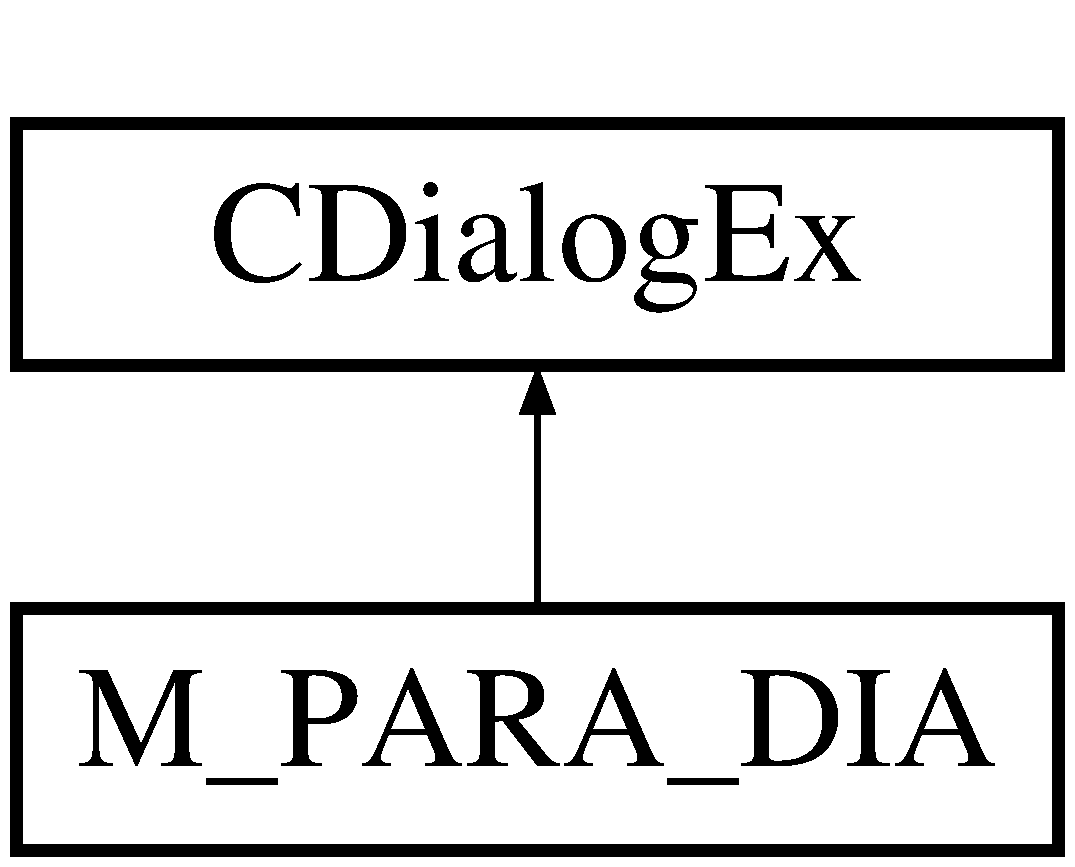
\includegraphics[height=2.000000cm]{class_m___p_a_r_a___d_i_a}
\end{center}
\end{figure}
\subsection*{Public Member Functions}
\begin{DoxyCompactItemize}
\item 
\mbox{\Hypertarget{class_m___p_a_r_a___d_i_a_a48afe90e65a6b5b795660771a979dead}\label{class_m___p_a_r_a___d_i_a_a48afe90e65a6b5b795660771a979dead}} 
\hyperlink{class_m___p_a_r_a___d_i_a_a48afe90e65a6b5b795660771a979dead}{M\+\_\+\+P\+A\+R\+A\+\_\+\+D\+IA} (C\+Wnd $\ast$p\+Parent=N\+U\+LL)
\begin{DoxyCompactList}\small\item\em 默认构造函数 \end{DoxyCompactList}\item 
\mbox{\Hypertarget{class_m___p_a_r_a___d_i_a_a773b615a0195eef82f905a622b986730}\label{class_m___p_a_r_a___d_i_a_a773b615a0195eef82f905a622b986730}} 
virtual \hyperlink{class_m___p_a_r_a___d_i_a_a773b615a0195eef82f905a622b986730}{$\sim$\+M\+\_\+\+P\+A\+R\+A\+\_\+\+D\+IA} ()
\begin{DoxyCompactList}\small\item\em 默认析构函数 \end{DoxyCompactList}\item 
\mbox{\Hypertarget{class_m___p_a_r_a___d_i_a_a65b051cfe602cb62465fbe415c5f9855}\label{class_m___p_a_r_a___d_i_a_a65b051cfe602cb62465fbe415c5f9855}} 
afx\+\_\+msg void {\bfseries On\+En\+Change\+Edit2} ()
\item 
\mbox{\Hypertarget{class_m___p_a_r_a___d_i_a_a27389e0288e070d6b6754db0a8e4d46a}\label{class_m___p_a_r_a___d_i_a_a27389e0288e070d6b6754db0a8e4d46a}} 
afx\+\_\+msg void {\bfseries On\+En\+Change\+Edit3} ()
\item 
\mbox{\Hypertarget{class_m___p_a_r_a___d_i_a_ada46b2ff3644d52d8afeb67bdae02c7b}\label{class_m___p_a_r_a___d_i_a_ada46b2ff3644d52d8afeb67bdae02c7b}} 
afx\+\_\+msg void {\bfseries On\+En\+Update\+Line} ()
\item 
\mbox{\Hypertarget{class_m___p_a_r_a___d_i_a_af5179b1264d23370b538c5a946122b32}\label{class_m___p_a_r_a___d_i_a_af5179b1264d23370b538c5a946122b32}} 
afx\+\_\+msg void {\bfseries On\+En\+Update\+Charac} ()
\item 
\mbox{\Hypertarget{class_m___p_a_r_a___d_i_a_afffa042b90b31b6d38bf33792096d908}\label{class_m___p_a_r_a___d_i_a_afffa042b90b31b6d38bf33792096d908}} 
afx\+\_\+msg void \hyperlink{class_m___p_a_r_a___d_i_a_afffa042b90b31b6d38bf33792096d908}{On\+Bn\+Clicked\+Ok} ()
\begin{DoxyCompactList}\small\item\em 当按下\+O\+K按钮的消息响应函数 \end{DoxyCompactList}\end{DoxyCompactItemize}
\subsection*{Public Attributes}
\begin{DoxyCompactItemize}
\item 
\mbox{\Hypertarget{class_m___p_a_r_a___d_i_a_aea31fe9cfbcfd5a9c9d218a0f5a821f7}\label{class_m___p_a_r_a___d_i_a_aea31fe9cfbcfd5a9c9d218a0f5a821f7}} 
int \hyperlink{class_m___p_a_r_a___d_i_a_aea31fe9cfbcfd5a9c9d218a0f5a821f7}{m\+\_\+linespace} = 0
\begin{DoxyCompactList}\small\item\em 行间距,默认值为0 \end{DoxyCompactList}\item 
\mbox{\Hypertarget{class_m___p_a_r_a___d_i_a_abdddacb23484b11c4ddf7be621fecd74}\label{class_m___p_a_r_a___d_i_a_abdddacb23484b11c4ddf7be621fecd74}} 
int \hyperlink{class_m___p_a_r_a___d_i_a_abdddacb23484b11c4ddf7be621fecd74}{m\+\_\+charaspace} = 0
\begin{DoxyCompactList}\small\item\em 字间距,默认值为0 \end{DoxyCompactList}\end{DoxyCompactItemize}
\subsection*{Protected Member Functions}
\begin{DoxyCompactItemize}
\item 
\mbox{\Hypertarget{class_m___p_a_r_a___d_i_a_a7d7ff9f843610a3ddccd12da36df7751}\label{class_m___p_a_r_a___d_i_a_a7d7ff9f843610a3ddccd12da36df7751}} 
virtual void \hyperlink{class_m___p_a_r_a___d_i_a_a7d7ff9f843610a3ddccd12da36df7751}{Do\+Data\+Exchange} (C\+Data\+Exchange $\ast$p\+DX)
\begin{DoxyCompactList}\small\item\em 数据交换函数 \end{DoxyCompactList}\end{DoxyCompactItemize}


\subsection{Detailed Description}
设置行间距以及字间距的对话框类\+M\+\_\+\+P\+A\+R\+A\+\_\+\+D\+IA ~\newline
该对话框用于用户设置行间距以及字间距~\newline
如果用户选择了一段文字,则输入的行距字间距将被用于选中的文字~\newline
如果用户没有选择文字,那么输入的行间距字间距将被应用于之后将会打出来的文字上~\newline


The documentation for this class was generated from the following files\+:\begin{DoxyCompactItemize}
\item 
Notepad/\hyperlink{_m___p_a_r_a___d_i_a_8h}{M\+\_\+\+P\+A\+R\+A\+\_\+\+D\+I\+A.\+h}\item 
Notepad/M\+\_\+\+P\+A\+R\+A\+\_\+\+D\+I\+A.\+cpp\end{DoxyCompactItemize}

\hypertarget{class_s_i_c_h_a_r___i_n_f_o}{}\section{S\+I\+C\+H\+A\+R\+\_\+\+I\+N\+F\+O类 参考}
\label{class_s_i_c_h_a_r___i_n_f_o}\index{S\+I\+C\+H\+A\+R\+\_\+\+I\+N\+FO@{S\+I\+C\+H\+A\+R\+\_\+\+I\+N\+FO}}


表示一个字符的可以\char`\"{}设置\char`\"{}的信息  




{\ttfamily \#include $<$kernal.\+h$>$}

\subsection*{Public 成员函数}
\begin{DoxyCompactItemize}
\item 
\mbox{\Hypertarget{class_s_i_c_h_a_r___i_n_f_o_ab0626402d19f4f4993077f947eb1c3de}\label{class_s_i_c_h_a_r___i_n_f_o_ab0626402d19f4f4993077f947eb1c3de}} 
\hyperlink{class_s_i_c_h_a_r___i_n_f_o_ab0626402d19f4f4993077f947eb1c3de}{S\+I\+C\+H\+A\+R\+\_\+\+I\+N\+FO} ()
\begin{DoxyCompactList}\small\item\em 构造函数1(默认)~\newline
\end{DoxyCompactList}\item 
\mbox{\Hypertarget{class_s_i_c_h_a_r___i_n_f_o_a21b428740b8332500ae61f43b700d6b2}\label{class_s_i_c_h_a_r___i_n_f_o_a21b428740b8332500ae61f43b700d6b2}} 
\hyperlink{class_s_i_c_h_a_r___i_n_f_o_a21b428740b8332500ae61f43b700d6b2}{S\+I\+C\+H\+A\+R\+\_\+\+I\+N\+FO} (const \hyperlink{class_s_i_c_h_a_r___i_n_f_o}{S\+I\+C\+H\+A\+R\+\_\+\+I\+N\+FO} \&tinfo)
\begin{DoxyCompactList}\small\item\em 构造函数2~\newline
\end{DoxyCompactList}\item 
void \hyperlink{class_s_i_c_h_a_r___i_n_f_o_a7dd5af8833b1951a6e4759668d484f37}{set\+\_\+fontpc} (S\+I\+F\+O\+N\+T\+\_\+P tfontpc)
\begin{DoxyCompactList}\small\item\em 设置fontpc成员(重载\+:1) \end{DoxyCompactList}\item 
void \hyperlink{class_s_i_c_h_a_r___i_n_f_o_a01ad1057400db3ccec680de26f4ab0a2}{set\+\_\+fontpc} (S\+I\+F\+O\+NT \&tfont)
\begin{DoxyCompactList}\small\item\em 设置fontpc成员(重载\+:2) \end{DoxyCompactList}\item 
void \hyperlink{class_s_i_c_h_a_r___i_n_f_o_a3c7718568eb9ff885af1bdfa8c197236}{set\+\_\+color} (C\+O\+L\+O\+R\+E\+RF tcolor)
\begin{DoxyCompactList}\small\item\em 设置color成员 \end{DoxyCompactList}\item 
void \hyperlink{class_s_i_c_h_a_r___i_n_f_o_afe883164593a8d3a5c9377eb5454c9f1}{set\+\_\+size} (C\+H\+A\+R\+S\+I\+ZE tsize)
\begin{DoxyCompactList}\small\item\em 设置size成员 \end{DoxyCompactList}\item 
void \hyperlink{class_s_i_c_h_a_r___i_n_f_o_a18aaf35f07094cb42942663a71456227}{set\+\_\+cspace} (C\+H\+A\+R\+S\+P\+A\+CE tcspace)
\begin{DoxyCompactList}\small\item\em 设置cspace成员 \end{DoxyCompactList}\item 
void \hyperlink{class_s_i_c_h_a_r___i_n_f_o_af38e1eac74e8d9c14e5c5d05d58f8b36}{set\+\_\+lspace} (L\+I\+N\+E\+S\+P\+A\+CE tlspace)
\begin{DoxyCompactList}\small\item\em 设置lspace成员 \end{DoxyCompactList}\item 
S\+I\+F\+O\+N\+T\+\_\+P \hyperlink{class_s_i_c_h_a_r___i_n_f_o_ad53aa1c6641e81bf0b79f17836aa5dfa}{get\+\_\+fontpc} ()
\begin{DoxyCompactList}\small\item\em 得到字体信息~\newline
\end{DoxyCompactList}\item 
C\+O\+L\+O\+R\+E\+RF \hyperlink{class_s_i_c_h_a_r___i_n_f_o_acd6d47c6cf5f266e18033e45763d6272}{get\+\_\+color} ()
\begin{DoxyCompactList}\small\item\em 得到颜色信息~\newline
\end{DoxyCompactList}\item 
C\+H\+A\+R\+S\+I\+ZE \hyperlink{class_s_i_c_h_a_r___i_n_f_o_aae2cfbd0b6bbb122008da027f662291b}{get\+\_\+size} ()
\begin{DoxyCompactList}\small\item\em 得到字体大小~\newline
\end{DoxyCompactList}\item 
C\+H\+A\+R\+S\+P\+A\+CE \hyperlink{class_s_i_c_h_a_r___i_n_f_o_af170e524f63209016d06f919dd4c33d3}{get\+\_\+cspace} ()
\begin{DoxyCompactList}\small\item\em 得到字间距~\newline
\end{DoxyCompactList}\item 
L\+I\+N\+E\+S\+P\+A\+CE \hyperlink{class_s_i_c_h_a_r___i_n_f_o_a212cea0692a8717d5b671035885796c2}{get\+\_\+lspace} ()
\begin{DoxyCompactList}\small\item\em 得到行间距~\newline
\end{DoxyCompactList}\item 
\mbox{\Hypertarget{class_s_i_c_h_a_r___i_n_f_o_afa85ade3f4a994f8454f835fe9c05a9e}\label{class_s_i_c_h_a_r___i_n_f_o_afa85ade3f4a994f8454f835fe9c05a9e}} 
void \hyperlink{class_s_i_c_h_a_r___i_n_f_o_afa85ade3f4a994f8454f835fe9c05a9e}{print\+\_\+info} ()
\begin{DoxyCompactList}\small\item\em 输出信息 \end{DoxyCompactList}\item 
\mbox{\Hypertarget{class_s_i_c_h_a_r___i_n_f_o_a762bed1602c6c28fbfda1bb1d29d7dff}\label{class_s_i_c_h_a_r___i_n_f_o_a762bed1602c6c28fbfda1bb1d29d7dff}} 
void \hyperlink{class_s_i_c_h_a_r___i_n_f_o_a762bed1602c6c28fbfda1bb1d29d7dff}{read\+\_\+info} ()
\begin{DoxyCompactList}\small\item\em 读入信息 \end{DoxyCompactList}\item 
\hyperlink{class_s_i_c_h_a_r___i_n_f_o}{S\+I\+C\+H\+A\+R\+\_\+\+I\+N\+FO} \& \hyperlink{class_s_i_c_h_a_r___i_n_f_o_a3083fe977f3675c45f0da8e9c38a399c}{operator=} (const \hyperlink{class_s_i_c_h_a_r___i_n_f_o}{S\+I\+C\+H\+A\+R\+\_\+\+I\+N\+FO} \&tinfo)
\begin{DoxyCompactList}\small\item\em 重载赋值函数~\newline
\end{DoxyCompactList}\end{DoxyCompactItemize}
\subsection*{Public 属性}
\begin{DoxyCompactItemize}
\item 
S\+I\+F\+O\+N\+T\+\_\+P \hyperlink{class_s_i_c_h_a_r___i_n_f_o_a8d998c494943882d98981f79f620460d}{fontpc}
\begin{DoxyCompactList}\small\item\em 字体信息,详见\+M\+S\+DN \end{DoxyCompactList}\item 
\mbox{\Hypertarget{class_s_i_c_h_a_r___i_n_f_o_ab9605aad10f9e033ed8e004468beeab9}\label{class_s_i_c_h_a_r___i_n_f_o_ab9605aad10f9e033ed8e004468beeab9}} 
C\+O\+L\+O\+R\+E\+RF \hyperlink{class_s_i_c_h_a_r___i_n_f_o_ab9605aad10f9e033ed8e004468beeab9}{color}
\begin{DoxyCompactList}\small\item\em 颜色信息  \end{DoxyCompactList}\item 
\mbox{\Hypertarget{class_s_i_c_h_a_r___i_n_f_o_a838a052749c0c04c6f20c633b1cc4432}\label{class_s_i_c_h_a_r___i_n_f_o_a838a052749c0c04c6f20c633b1cc4432}} 
C\+O\+L\+O\+R\+E\+RF \hyperlink{class_s_i_c_h_a_r___i_n_f_o_a838a052749c0c04c6f20c633b1cc4432}{bgcolor}
\begin{DoxyCompactList}\small\item\em 背景颜色信息  \end{DoxyCompactList}\item 
\mbox{\Hypertarget{class_s_i_c_h_a_r___i_n_f_o_abcc72d98471148d54e334f9528103a50}\label{class_s_i_c_h_a_r___i_n_f_o_abcc72d98471148d54e334f9528103a50}} 
C\+H\+A\+R\+S\+I\+ZE \hyperlink{class_s_i_c_h_a_r___i_n_f_o_abcc72d98471148d54e334f9528103a50}{size}
\begin{DoxyCompactList}\small\item\em 字体大小,这里用作标识符  \end{DoxyCompactList}\item 
\mbox{\Hypertarget{class_s_i_c_h_a_r___i_n_f_o_a575d876eda778563dec0f72bd4bc06ea}\label{class_s_i_c_h_a_r___i_n_f_o_a575d876eda778563dec0f72bd4bc06ea}} 
C\+H\+A\+R\+S\+P\+A\+CE \hyperlink{class_s_i_c_h_a_r___i_n_f_o_a575d876eda778563dec0f72bd4bc06ea}{cspace}
\begin{DoxyCompactList}\small\item\em 字间距  \end{DoxyCompactList}\item 
\mbox{\Hypertarget{class_s_i_c_h_a_r___i_n_f_o_ace4bad34a55f914a2fbbdeb8f9a22bae}\label{class_s_i_c_h_a_r___i_n_f_o_ace4bad34a55f914a2fbbdeb8f9a22bae}} 
L\+I\+N\+E\+S\+P\+A\+CE \hyperlink{class_s_i_c_h_a_r___i_n_f_o_ace4bad34a55f914a2fbbdeb8f9a22bae}{lspace}
\begin{DoxyCompactList}\small\item\em 行间距  \end{DoxyCompactList}\item 
\mbox{\Hypertarget{class_s_i_c_h_a_r___i_n_f_o_a698a16c3b045894991c8aa2982190c7e}\label{class_s_i_c_h_a_r___i_n_f_o_a698a16c3b045894991c8aa2982190c7e}} 
S\+I\+A\+L\+I\+GN \hyperlink{class_s_i_c_h_a_r___i_n_f_o_a698a16c3b045894991c8aa2982190c7e}{align}
\begin{DoxyCompactList}\small\item\em 对齐方式  \end{DoxyCompactList}\end{DoxyCompactItemize}
\subsection*{友元}
\begin{DoxyCompactItemize}
\item 
\mbox{\Hypertarget{class_s_i_c_h_a_r___i_n_f_o_a33fe671aa658d4d9c3e3723f54dd2f31}\label{class_s_i_c_h_a_r___i_n_f_o_a33fe671aa658d4d9c3e3723f54dd2f31}} 
class {\bfseries S\+I\+C\+H\+A\+R\+N\+O\+DE}
\end{DoxyCompactItemize}


\subsection{详细描述}
表示一个字符的可以\char`\"{}设置\char`\"{}的信息 

\subsection{成员函数说明}
\mbox{\Hypertarget{class_s_i_c_h_a_r___i_n_f_o_acd6d47c6cf5f266e18033e45763d6272}\label{class_s_i_c_h_a_r___i_n_f_o_acd6d47c6cf5f266e18033e45763d6272}} 
\index{S\+I\+C\+H\+A\+R\+\_\+\+I\+N\+FO@{S\+I\+C\+H\+A\+R\+\_\+\+I\+N\+FO}!get\+\_\+color@{get\+\_\+color}}
\index{get\+\_\+color@{get\+\_\+color}!S\+I\+C\+H\+A\+R\+\_\+\+I\+N\+FO@{S\+I\+C\+H\+A\+R\+\_\+\+I\+N\+FO}}
\subsubsection{\texorpdfstring{get\+\_\+color()}{get\_color()}}
{\footnotesize\ttfamily C\+O\+L\+O\+R\+E\+RF S\+I\+C\+H\+A\+R\+\_\+\+I\+N\+F\+O\+::get\+\_\+color (\begin{DoxyParamCaption}{ }\end{DoxyParamCaption})\hspace{0.3cm}{\ttfamily [inline]}}



得到颜色信息~\newline



\begin{DoxyRetVals}{返回值}
{\em 一个\+C\+O\+L\+O\+R\+R\+E\+F类型的变量,表示颜色} & \\
\hline
\end{DoxyRetVals}
\mbox{\Hypertarget{class_s_i_c_h_a_r___i_n_f_o_af170e524f63209016d06f919dd4c33d3}\label{class_s_i_c_h_a_r___i_n_f_o_af170e524f63209016d06f919dd4c33d3}} 
\index{S\+I\+C\+H\+A\+R\+\_\+\+I\+N\+FO@{S\+I\+C\+H\+A\+R\+\_\+\+I\+N\+FO}!get\+\_\+cspace@{get\+\_\+cspace}}
\index{get\+\_\+cspace@{get\+\_\+cspace}!S\+I\+C\+H\+A\+R\+\_\+\+I\+N\+FO@{S\+I\+C\+H\+A\+R\+\_\+\+I\+N\+FO}}
\subsubsection{\texorpdfstring{get\+\_\+cspace()}{get\_cspace()}}
{\footnotesize\ttfamily C\+H\+A\+R\+S\+P\+A\+CE S\+I\+C\+H\+A\+R\+\_\+\+I\+N\+F\+O\+::get\+\_\+cspace (\begin{DoxyParamCaption}{ }\end{DoxyParamCaption})\hspace{0.3cm}{\ttfamily [inline]}}



得到字间距~\newline



\begin{DoxyRetVals}{返回值}
{\em 一个\+C\+H\+A\+R\+S\+P\+A\+C\+E类型的变量,表示字间距} & \\
\hline
\end{DoxyRetVals}
\mbox{\Hypertarget{class_s_i_c_h_a_r___i_n_f_o_ad53aa1c6641e81bf0b79f17836aa5dfa}\label{class_s_i_c_h_a_r___i_n_f_o_ad53aa1c6641e81bf0b79f17836aa5dfa}} 
\index{S\+I\+C\+H\+A\+R\+\_\+\+I\+N\+FO@{S\+I\+C\+H\+A\+R\+\_\+\+I\+N\+FO}!get\+\_\+fontpc@{get\+\_\+fontpc}}
\index{get\+\_\+fontpc@{get\+\_\+fontpc}!S\+I\+C\+H\+A\+R\+\_\+\+I\+N\+FO@{S\+I\+C\+H\+A\+R\+\_\+\+I\+N\+FO}}
\subsubsection{\texorpdfstring{get\+\_\+fontpc()}{get\_fontpc()}}
{\footnotesize\ttfamily S\+I\+F\+O\+N\+T\+\_\+P S\+I\+C\+H\+A\+R\+\_\+\+I\+N\+F\+O\+::get\+\_\+fontpc (\begin{DoxyParamCaption}{ }\end{DoxyParamCaption})\hspace{0.3cm}{\ttfamily [inline]}}



得到字体信息~\newline



\begin{DoxyRetVals}{返回值}
{\em 一个指向\+S\+I\+F\+O\+N\+T的指针,表示字体信息} & \\
\hline
\end{DoxyRetVals}
\mbox{\Hypertarget{class_s_i_c_h_a_r___i_n_f_o_a212cea0692a8717d5b671035885796c2}\label{class_s_i_c_h_a_r___i_n_f_o_a212cea0692a8717d5b671035885796c2}} 
\index{S\+I\+C\+H\+A\+R\+\_\+\+I\+N\+FO@{S\+I\+C\+H\+A\+R\+\_\+\+I\+N\+FO}!get\+\_\+lspace@{get\+\_\+lspace}}
\index{get\+\_\+lspace@{get\+\_\+lspace}!S\+I\+C\+H\+A\+R\+\_\+\+I\+N\+FO@{S\+I\+C\+H\+A\+R\+\_\+\+I\+N\+FO}}
\subsubsection{\texorpdfstring{get\+\_\+lspace()}{get\_lspace()}}
{\footnotesize\ttfamily L\+I\+N\+E\+S\+P\+A\+CE S\+I\+C\+H\+A\+R\+\_\+\+I\+N\+F\+O\+::get\+\_\+lspace (\begin{DoxyParamCaption}{ }\end{DoxyParamCaption})\hspace{0.3cm}{\ttfamily [inline]}}



得到行间距~\newline



\begin{DoxyRetVals}{返回值}
{\em 一个\+L\+I\+N\+E\+S\+P\+A\+C\+E类型的变量,表示行间距} & \\
\hline
\end{DoxyRetVals}
\mbox{\Hypertarget{class_s_i_c_h_a_r___i_n_f_o_aae2cfbd0b6bbb122008da027f662291b}\label{class_s_i_c_h_a_r___i_n_f_o_aae2cfbd0b6bbb122008da027f662291b}} 
\index{S\+I\+C\+H\+A\+R\+\_\+\+I\+N\+FO@{S\+I\+C\+H\+A\+R\+\_\+\+I\+N\+FO}!get\+\_\+size@{get\+\_\+size}}
\index{get\+\_\+size@{get\+\_\+size}!S\+I\+C\+H\+A\+R\+\_\+\+I\+N\+FO@{S\+I\+C\+H\+A\+R\+\_\+\+I\+N\+FO}}
\subsubsection{\texorpdfstring{get\+\_\+size()}{get\_size()}}
{\footnotesize\ttfamily C\+H\+A\+R\+S\+I\+ZE S\+I\+C\+H\+A\+R\+\_\+\+I\+N\+F\+O\+::get\+\_\+size (\begin{DoxyParamCaption}{ }\end{DoxyParamCaption})\hspace{0.3cm}{\ttfamily [inline]}}



得到字体大小~\newline



\begin{DoxyRetVals}{返回值}
{\em 一个\+C\+H\+A\+R\+S\+I\+Z\+E类型的变量,表示字体大小} & \\
\hline
\end{DoxyRetVals}
\mbox{\Hypertarget{class_s_i_c_h_a_r___i_n_f_o_a3083fe977f3675c45f0da8e9c38a399c}\label{class_s_i_c_h_a_r___i_n_f_o_a3083fe977f3675c45f0da8e9c38a399c}} 
\index{S\+I\+C\+H\+A\+R\+\_\+\+I\+N\+FO@{S\+I\+C\+H\+A\+R\+\_\+\+I\+N\+FO}!operator=@{operator=}}
\index{operator=@{operator=}!S\+I\+C\+H\+A\+R\+\_\+\+I\+N\+FO@{S\+I\+C\+H\+A\+R\+\_\+\+I\+N\+FO}}
\subsubsection{\texorpdfstring{operator=()}{operator=()}}
{\footnotesize\ttfamily \hyperlink{class_s_i_c_h_a_r___i_n_f_o}{S\+I\+C\+H\+A\+R\+\_\+\+I\+N\+FO} \& S\+I\+C\+H\+A\+R\+\_\+\+I\+N\+F\+O\+::operator= (\begin{DoxyParamCaption}\item[{const \hyperlink{class_s_i_c_h_a_r___i_n_f_o}{S\+I\+C\+H\+A\+R\+\_\+\+I\+N\+FO} \&}]{tinfo }\end{DoxyParamCaption})}



重载赋值函数~\newline


\begin{DoxyNote}{注解}
这个函数中,fontpc是复制指针指向的内容而不是指针本身 
\end{DoxyNote}

\begin{DoxyParams}[1]{参数}
\mbox{\tt in}  & {\em $\ast$this} & 左操作数 \\
\hline
\mbox{\tt in}  & {\em tinfo} & 右操作数 \\
\hline
\end{DoxyParams}

\begin{DoxyRetVals}{返回值}
{\em $\ast$this} & \\
\hline
\end{DoxyRetVals}
\mbox{\Hypertarget{class_s_i_c_h_a_r___i_n_f_o_a3c7718568eb9ff885af1bdfa8c197236}\label{class_s_i_c_h_a_r___i_n_f_o_a3c7718568eb9ff885af1bdfa8c197236}} 
\index{S\+I\+C\+H\+A\+R\+\_\+\+I\+N\+FO@{S\+I\+C\+H\+A\+R\+\_\+\+I\+N\+FO}!set\+\_\+color@{set\+\_\+color}}
\index{set\+\_\+color@{set\+\_\+color}!S\+I\+C\+H\+A\+R\+\_\+\+I\+N\+FO@{S\+I\+C\+H\+A\+R\+\_\+\+I\+N\+FO}}
\subsubsection{\texorpdfstring{set\+\_\+color()}{set\_color()}}
{\footnotesize\ttfamily void S\+I\+C\+H\+A\+R\+\_\+\+I\+N\+F\+O\+::set\+\_\+color (\begin{DoxyParamCaption}\item[{C\+O\+L\+O\+R\+E\+RF}]{tcolor }\end{DoxyParamCaption})\hspace{0.3cm}{\ttfamily [inline]}}



设置color成员 

\begin{DoxySeeAlso}{参见}
\hyperlink{class_s_i_c_h_a_r___i_n_f_o_ab9605aad10f9e033ed8e004468beeab9}{color} 
\end{DoxySeeAlso}
\mbox{\Hypertarget{class_s_i_c_h_a_r___i_n_f_o_a18aaf35f07094cb42942663a71456227}\label{class_s_i_c_h_a_r___i_n_f_o_a18aaf35f07094cb42942663a71456227}} 
\index{S\+I\+C\+H\+A\+R\+\_\+\+I\+N\+FO@{S\+I\+C\+H\+A\+R\+\_\+\+I\+N\+FO}!set\+\_\+cspace@{set\+\_\+cspace}}
\index{set\+\_\+cspace@{set\+\_\+cspace}!S\+I\+C\+H\+A\+R\+\_\+\+I\+N\+FO@{S\+I\+C\+H\+A\+R\+\_\+\+I\+N\+FO}}
\subsubsection{\texorpdfstring{set\+\_\+cspace()}{set\_cspace()}}
{\footnotesize\ttfamily void S\+I\+C\+H\+A\+R\+\_\+\+I\+N\+F\+O\+::set\+\_\+cspace (\begin{DoxyParamCaption}\item[{C\+H\+A\+R\+S\+P\+A\+CE}]{tcspace }\end{DoxyParamCaption})\hspace{0.3cm}{\ttfamily [inline]}}



设置cspace成员 

\begin{DoxySeeAlso}{参见}
\hyperlink{class_s_i_c_h_a_r___i_n_f_o_a575d876eda778563dec0f72bd4bc06ea}{cspace} 
\end{DoxySeeAlso}
\mbox{\Hypertarget{class_s_i_c_h_a_r___i_n_f_o_a7dd5af8833b1951a6e4759668d484f37}\label{class_s_i_c_h_a_r___i_n_f_o_a7dd5af8833b1951a6e4759668d484f37}} 
\index{S\+I\+C\+H\+A\+R\+\_\+\+I\+N\+FO@{S\+I\+C\+H\+A\+R\+\_\+\+I\+N\+FO}!set\+\_\+fontpc@{set\+\_\+fontpc}}
\index{set\+\_\+fontpc@{set\+\_\+fontpc}!S\+I\+C\+H\+A\+R\+\_\+\+I\+N\+FO@{S\+I\+C\+H\+A\+R\+\_\+\+I\+N\+FO}}
\subsubsection{\texorpdfstring{set\+\_\+fontpc()}{set\_fontpc()}\hspace{0.1cm}{\footnotesize\ttfamily [1/2]}}
{\footnotesize\ttfamily void S\+I\+C\+H\+A\+R\+\_\+\+I\+N\+F\+O\+::set\+\_\+fontpc (\begin{DoxyParamCaption}\item[{S\+I\+F\+O\+N\+T\+\_\+P}]{tfontpc }\end{DoxyParamCaption})\hspace{0.3cm}{\ttfamily [inline]}}



设置fontpc成员(重载\+:1) 

\begin{DoxySeeAlso}{参见}
\hyperlink{class_s_i_c_h_a_r___i_n_f_o_a8d998c494943882d98981f79f620460d}{fontpc} 
\end{DoxySeeAlso}
\mbox{\Hypertarget{class_s_i_c_h_a_r___i_n_f_o_a01ad1057400db3ccec680de26f4ab0a2}\label{class_s_i_c_h_a_r___i_n_f_o_a01ad1057400db3ccec680de26f4ab0a2}} 
\index{S\+I\+C\+H\+A\+R\+\_\+\+I\+N\+FO@{S\+I\+C\+H\+A\+R\+\_\+\+I\+N\+FO}!set\+\_\+fontpc@{set\+\_\+fontpc}}
\index{set\+\_\+fontpc@{set\+\_\+fontpc}!S\+I\+C\+H\+A\+R\+\_\+\+I\+N\+FO@{S\+I\+C\+H\+A\+R\+\_\+\+I\+N\+FO}}
\subsubsection{\texorpdfstring{set\+\_\+fontpc()}{set\_fontpc()}\hspace{0.1cm}{\footnotesize\ttfamily [2/2]}}
{\footnotesize\ttfamily void S\+I\+C\+H\+A\+R\+\_\+\+I\+N\+F\+O\+::set\+\_\+fontpc (\begin{DoxyParamCaption}\item[{S\+I\+F\+O\+NT \&}]{tfont }\end{DoxyParamCaption})\hspace{0.3cm}{\ttfamily [inline]}}



设置fontpc成员(重载\+:2) 

\begin{DoxySeeAlso}{参见}
\hyperlink{class_s_i_c_h_a_r___i_n_f_o_a8d998c494943882d98981f79f620460d}{fontpc} 
\end{DoxySeeAlso}
\mbox{\Hypertarget{class_s_i_c_h_a_r___i_n_f_o_af38e1eac74e8d9c14e5c5d05d58f8b36}\label{class_s_i_c_h_a_r___i_n_f_o_af38e1eac74e8d9c14e5c5d05d58f8b36}} 
\index{S\+I\+C\+H\+A\+R\+\_\+\+I\+N\+FO@{S\+I\+C\+H\+A\+R\+\_\+\+I\+N\+FO}!set\+\_\+lspace@{set\+\_\+lspace}}
\index{set\+\_\+lspace@{set\+\_\+lspace}!S\+I\+C\+H\+A\+R\+\_\+\+I\+N\+FO@{S\+I\+C\+H\+A\+R\+\_\+\+I\+N\+FO}}
\subsubsection{\texorpdfstring{set\+\_\+lspace()}{set\_lspace()}}
{\footnotesize\ttfamily void S\+I\+C\+H\+A\+R\+\_\+\+I\+N\+F\+O\+::set\+\_\+lspace (\begin{DoxyParamCaption}\item[{L\+I\+N\+E\+S\+P\+A\+CE}]{tlspace }\end{DoxyParamCaption})\hspace{0.3cm}{\ttfamily [inline]}}



设置lspace成员 

\begin{DoxySeeAlso}{参见}
\hyperlink{class_s_i_c_h_a_r___i_n_f_o_ace4bad34a55f914a2fbbdeb8f9a22bae}{lspace} 
\end{DoxySeeAlso}
\mbox{\Hypertarget{class_s_i_c_h_a_r___i_n_f_o_afe883164593a8d3a5c9377eb5454c9f1}\label{class_s_i_c_h_a_r___i_n_f_o_afe883164593a8d3a5c9377eb5454c9f1}} 
\index{S\+I\+C\+H\+A\+R\+\_\+\+I\+N\+FO@{S\+I\+C\+H\+A\+R\+\_\+\+I\+N\+FO}!set\+\_\+size@{set\+\_\+size}}
\index{set\+\_\+size@{set\+\_\+size}!S\+I\+C\+H\+A\+R\+\_\+\+I\+N\+FO@{S\+I\+C\+H\+A\+R\+\_\+\+I\+N\+FO}}
\subsubsection{\texorpdfstring{set\+\_\+size()}{set\_size()}}
{\footnotesize\ttfamily void S\+I\+C\+H\+A\+R\+\_\+\+I\+N\+F\+O\+::set\+\_\+size (\begin{DoxyParamCaption}\item[{C\+H\+A\+R\+S\+I\+ZE}]{tsize }\end{DoxyParamCaption})\hspace{0.3cm}{\ttfamily [inline]}}



设置size成员 

\begin{DoxySeeAlso}{参见}
\hyperlink{class_s_i_c_h_a_r___i_n_f_o_abcc72d98471148d54e334f9528103a50}{size} 
\end{DoxySeeAlso}


\subsection{类成员变量说明}
\mbox{\Hypertarget{class_s_i_c_h_a_r___i_n_f_o_a8d998c494943882d98981f79f620460d}\label{class_s_i_c_h_a_r___i_n_f_o_a8d998c494943882d98981f79f620460d}} 
\index{S\+I\+C\+H\+A\+R\+\_\+\+I\+N\+FO@{S\+I\+C\+H\+A\+R\+\_\+\+I\+N\+FO}!fontpc@{fontpc}}
\index{fontpc@{fontpc}!S\+I\+C\+H\+A\+R\+\_\+\+I\+N\+FO@{S\+I\+C\+H\+A\+R\+\_\+\+I\+N\+FO}}
\subsubsection{\texorpdfstring{fontpc}{fontpc}}
{\footnotesize\ttfamily S\+I\+F\+O\+N\+T\+\_\+P S\+I\+C\+H\+A\+R\+\_\+\+I\+N\+F\+O\+::fontpc}



字体信息,详见\+M\+S\+DN 

\begin{DoxySeeAlso}{参见}
S\+I\+F\+O\+N\+T\+\_\+P 
\end{DoxySeeAlso}


该类的文档由以下文件生成\+:\begin{DoxyCompactItemize}
\item 
Notepad/\hyperlink{kernal_8h}{kernal.\+h}\item 
Notepad/kernal.\+cpp\end{DoxyCompactItemize}

\hypertarget{class_s_i_c_h_a_r_n_o_d_e}{}\section{S\+I\+C\+H\+A\+R\+N\+O\+D\+E类 参考}
\label{class_s_i_c_h_a_r_n_o_d_e}\index{S\+I\+C\+H\+A\+R\+N\+O\+DE@{S\+I\+C\+H\+A\+R\+N\+O\+DE}}


表示文本链表的一个节点~\newline
 




{\ttfamily \#include $<$kernal.\+h$>$}

\subsection*{Public 成员函数}
\begin{DoxyCompactItemize}
\item 
\mbox{\Hypertarget{class_s_i_c_h_a_r_n_o_d_e_a69da1200fe43cf1aab75e44650cdd21b}\label{class_s_i_c_h_a_r_n_o_d_e_a69da1200fe43cf1aab75e44650cdd21b}} 
\hyperlink{class_s_i_c_h_a_r_n_o_d_e_a69da1200fe43cf1aab75e44650cdd21b}{S\+I\+C\+H\+A\+R\+N\+O\+DE} (S\+I\+C\+H\+A\+R\+\_\+T tch, \hyperlink{class_s_i_c_h_a_r_n_o_d_e}{S\+I\+C\+H\+A\+R\+N\+O\+DE} $\ast$tprevp=N\+U\+LL, \hyperlink{class_s_i_c_h_a_r_n_o_d_e}{S\+I\+C\+H\+A\+R\+N\+O\+DE} $\ast$tnextp=N\+U\+LL, \hyperlink{class_s_i_c_h_a_r___i_n_f_o}{S\+I\+C\+H\+A\+R\+\_\+\+I\+N\+F\+O\+\_\+P} tchar\+\_\+infop=N\+U\+LL, \hyperlink{class_s_i_d_r_a_w___i_n_f_o}{S\+I\+D\+R\+A\+W\+\_\+\+I\+N\+F\+O\+\_\+P} tdraw\+\_\+infop=N\+U\+LL)
\begin{DoxyCompactList}\small\item\em 构造函数1 \end{DoxyCompactList}\item 
\mbox{\Hypertarget{class_s_i_c_h_a_r_n_o_d_e_aa06366dc16bf0aab9d16aaf43be0f8a3}\label{class_s_i_c_h_a_r_n_o_d_e_aa06366dc16bf0aab9d16aaf43be0f8a3}} 
\hyperlink{class_s_i_c_h_a_r_n_o_d_e_aa06366dc16bf0aab9d16aaf43be0f8a3}{S\+I\+C\+H\+A\+R\+N\+O\+DE} (S\+I\+C\+H\+A\+R\+\_\+T tch, int tswidth, int tsheight)
\begin{DoxyCompactList}\small\item\em 构造函数2 \end{DoxyCompactList}\item 
void \hyperlink{class_s_i_c_h_a_r_n_o_d_e_ab0d781b8bb3d87470d1826cea65b61aa}{calc\+\_\+\+S\+\_\+from\+\_\+font} ()
\begin{DoxyCompactList}\small\item\em 从当前的字体计算出绘制信息中的\+S的大小 \end{DoxyCompactList}\item 
\mbox{\Hypertarget{class_s_i_c_h_a_r_n_o_d_e_aad179bc8f8fc9a4789e0b9ba06ecef9a}\label{class_s_i_c_h_a_r_n_o_d_e_aad179bc8f8fc9a4789e0b9ba06ecef9a}} 
void \hyperlink{class_s_i_c_h_a_r_n_o_d_e_aad179bc8f8fc9a4789e0b9ba06ecef9a}{set\+\_\+fontpc} (S\+I\+F\+O\+N\+T\+\_\+P tfontpc)
\begin{DoxyCompactList}\small\item\em 设置char\+\_\+infop中的fontpc并重新计算draw\+\_\+infop中的\+S的大小 \end{DoxyCompactList}\item 
\mbox{\Hypertarget{class_s_i_c_h_a_r_n_o_d_e_a31c2182d80551b2d92cc13f8c966d5e7}\label{class_s_i_c_h_a_r_n_o_d_e_a31c2182d80551b2d92cc13f8c966d5e7}} 
void {\bfseries set\+\_\+fontpc} (S\+I\+F\+O\+NT \&tfont)
\item 
\mbox{\Hypertarget{class_s_i_c_h_a_r_n_o_d_e_a178979e4d98192f354dcccf93b18202b}\label{class_s_i_c_h_a_r_n_o_d_e_a178979e4d98192f354dcccf93b18202b}} 
void {\bfseries set\+\_\+color} (C\+O\+L\+O\+R\+E\+RF tcolor)
\item 
\mbox{\Hypertarget{class_s_i_c_h_a_r_n_o_d_e_a22ad69de5483e52b83a380d700112d33}\label{class_s_i_c_h_a_r_n_o_d_e_a22ad69de5483e52b83a380d700112d33}} 
void {\bfseries set\+\_\+size} (C\+H\+A\+R\+S\+I\+ZE tsize)
\item 
\mbox{\Hypertarget{class_s_i_c_h_a_r_n_o_d_e_ab6b5d998c28439e54749bb5502cdeec2}\label{class_s_i_c_h_a_r_n_o_d_e_ab6b5d998c28439e54749bb5502cdeec2}} 
void {\bfseries set\+\_\+draw\+\_\+infop\+\_\+S} (const \hyperlink{struct_s_i_r_e_c_t}{S\+I\+R\+E\+CT} \&TS)
\item 
\mbox{\Hypertarget{class_s_i_c_h_a_r_n_o_d_e_abe788ffb5847e2be9bb047d57e8666f7}\label{class_s_i_c_h_a_r_n_o_d_e_abe788ffb5847e2be9bb047d57e8666f7}} 
void {\bfseries set\+\_\+draw\+\_\+infop\+\_\+L} (const \hyperlink{struct_s_i_r_e_c_t}{S\+I\+R\+E\+CT} \&TL)
\item 
\mbox{\Hypertarget{class_s_i_c_h_a_r_n_o_d_e_a52e5c4ff341d7276063e6441452b4c3f}\label{class_s_i_c_h_a_r_n_o_d_e_a52e5c4ff341d7276063e6441452b4c3f}} 
void {\bfseries set\+\_\+draw\+\_\+infop\+\_\+P} (const \hyperlink{struct_s_i_p_o_i_n_t}{S\+I\+P\+O\+I\+NT} \&TP)
\item 
\mbox{\Hypertarget{class_s_i_c_h_a_r_n_o_d_e_aa84ae4bcf6cc7eba84a0c93f3d1c6bc9}\label{class_s_i_c_h_a_r_n_o_d_e_aa84ae4bcf6cc7eba84a0c93f3d1c6bc9}} 
void {\bfseries set\+\_\+align} (S\+I\+A\+L\+I\+GN align)
\item 
void \hyperlink{class_s_i_c_h_a_r_n_o_d_e_a0aba68c10438db18bea07bb77d70f839}{ins\+\_\+prev} (\hyperlink{class_s_i_c_h_a_r_n_o_d_e}{S\+I\+C\+H\+A\+R\+N\+O\+DE} $\ast$p)
\begin{DoxyCompactList}\small\item\em 在当前字符的前面插入一个节点~\newline
\end{DoxyCompactList}\item 
void \hyperlink{class_s_i_c_h_a_r_n_o_d_e_a9a3f1b6c50c483ad2d8a770f4590c50c}{ins\+\_\+next} (\hyperlink{class_s_i_c_h_a_r_n_o_d_e}{S\+I\+C\+H\+A\+R\+N\+O\+DE} $\ast$p)
\begin{DoxyCompactList}\small\item\em 在当前字符的后面插入一个节点~\newline
\end{DoxyCompactList}\item 
void \hyperlink{class_s_i_c_h_a_r_n_o_d_e_ae703c63e9c8e05fc6069e539fc3f6a01}{ins\+\_\+prev} (\hyperlink{class_s_i_c_h_a_r_n_o_d_e}{S\+I\+C\+H\+A\+R\+N\+O\+DE} $\ast$ps, \hyperlink{class_s_i_c_h_a_r_n_o_d_e}{S\+I\+C\+H\+A\+R\+N\+O\+DE} $\ast$pe)
\begin{DoxyCompactList}\small\item\em 在当前字符的前面插入一段节点~\newline
\end{DoxyCompactList}\item 
void \hyperlink{class_s_i_c_h_a_r_n_o_d_e_a5c7b26fb6c8d148b4bb2f81ac21939b9}{ins\+\_\+next} (\hyperlink{class_s_i_c_h_a_r_n_o_d_e}{S\+I\+C\+H\+A\+R\+N\+O\+DE} $\ast$ps, \hyperlink{class_s_i_c_h_a_r_n_o_d_e}{S\+I\+C\+H\+A\+R\+N\+O\+DE} $\ast$pe)
\begin{DoxyCompactList}\small\item\em 在当前字符的后面插入一段节点~\newline
\end{DoxyCompactList}\item 
void \hyperlink{class_s_i_c_h_a_r_n_o_d_e_a85ebada9a5d765d7f055bab903b6c6d2}{ins\+\_\+prev} (const \hyperlink{struct_s_i_r_a_n_g_e}{S\+I\+R\+A\+N\+GE} \&range)
\begin{DoxyCompactList}\small\item\em 等价于{\ttfamily ins\+\_\+prev(range.\+sp,range.\+ep)}~\newline
\end{DoxyCompactList}\item 
void \hyperlink{class_s_i_c_h_a_r_n_o_d_e_af8048308dc6b0ffdf02caceb814ee8e3}{ins\+\_\+next} (const \hyperlink{struct_s_i_r_a_n_g_e}{S\+I\+R\+A\+N\+GE} \&range)
\begin{DoxyCompactList}\small\item\em 等价于{\ttfamily ins\+\_\+next(range.\+sp,range.\+ep)}~\newline
\end{DoxyCompactList}\item 
const \hyperlink{class_s_i_c_h_a_r___i_n_f_o}{S\+I\+C\+H\+A\+R\+\_\+\+I\+N\+F\+O\+\_\+P} \hyperlink{class_s_i_c_h_a_r_n_o_d_e_a95039205cd53a18d6f1b8ef1a80c90c2}{get\+\_\+char\+\_\+infop} ()
\begin{DoxyCompactList}\small\item\em 得到一个char\+\_\+infop的const副本 \end{DoxyCompactList}\item 
const \hyperlink{class_s_i_d_r_a_w___i_n_f_o}{S\+I\+D\+R\+A\+W\+\_\+\+I\+N\+F\+O\+\_\+P} \hyperlink{class_s_i_c_h_a_r_n_o_d_e_a96a8903f87343bb9096a8ed014e789be}{get\+\_\+draw\+\_\+infop} ()
\begin{DoxyCompactList}\small\item\em 得到一个draw\+\_\+infop的const副本 \end{DoxyCompactList}\item 
\mbox{\Hypertarget{class_s_i_c_h_a_r_n_o_d_e_a4b4d71bb1d49d56399586b214897bec4}\label{class_s_i_c_h_a_r_n_o_d_e_a4b4d71bb1d49d56399586b214897bec4}} 
void \hyperlink{class_s_i_c_h_a_r_n_o_d_e_a4b4d71bb1d49d56399586b214897bec4}{print\+\_\+info} ()
\begin{DoxyCompactList}\small\item\em 输出信息 \end{DoxyCompactList}\item 
\mbox{\Hypertarget{class_s_i_c_h_a_r_n_o_d_e_ae51d8c92371116aedf5510bb3096104c}\label{class_s_i_c_h_a_r_n_o_d_e_ae51d8c92371116aedf5510bb3096104c}} 
void \hyperlink{class_s_i_c_h_a_r_n_o_d_e_ae51d8c92371116aedf5510bb3096104c}{read\+\_\+info} ()
\begin{DoxyCompactList}\small\item\em 输入信息 \end{DoxyCompactList}\end{DoxyCompactItemize}
\subsection*{Public 属性}
\begin{DoxyCompactItemize}
\item 
S\+I\+C\+H\+A\+R\+\_\+T \hyperlink{class_s_i_c_h_a_r_n_o_d_e_a87aabfc0878d7c6cce226256873797e0}{ch}
\begin{DoxyCompactList}\small\item\em 字符 \end{DoxyCompactList}\item 
\hyperlink{class_s_i_c_h_a_r___i_n_f_o}{S\+I\+C\+H\+A\+R\+\_\+\+I\+N\+F\+O\+\_\+P} \hyperlink{class_s_i_c_h_a_r_n_o_d_e_a03e4b28edd8566a6b605f4caeeb7bd6f}{char\+\_\+infop}
\begin{DoxyCompactList}\small\item\em 字体信息~\newline
一个指向\+S\+I\+C\+H\+A\+R\+\_\+\+I\+N\+F\+O类型的指针,储存该字符的字体信息 \end{DoxyCompactList}\item 
\hyperlink{class_s_i_d_r_a_w___i_n_f_o}{S\+I\+D\+R\+A\+W\+\_\+\+I\+N\+F\+O\+\_\+P} \hyperlink{class_s_i_c_h_a_r_n_o_d_e_aee3adfece6b51d9f71a0aa19d203b106}{draw\+\_\+infop}
\begin{DoxyCompactList}\small\item\em 绘制信息~\newline
一个指向\+S\+I\+D\+R\+A\+W\+\_\+\+I\+N\+F\+O类型的指针,储存该字符的绘制信息 \end{DoxyCompactList}\item 
\mbox{\Hypertarget{class_s_i_c_h_a_r_n_o_d_e_ad4d1b1aee15e867902bbf17938a86e64}\label{class_s_i_c_h_a_r_n_o_d_e_ad4d1b1aee15e867902bbf17938a86e64}} 
\hyperlink{class_s_i_c_h_a_r_n_o_d_e}{S\+I\+C\+H\+A\+R\+N\+O\+DE} $\ast$ \hyperlink{class_s_i_c_h_a_r_n_o_d_e_ad4d1b1aee15e867902bbf17938a86e64}{prevp}
\begin{DoxyCompactList}\small\item\em 指向链表前一个节点的指针 \end{DoxyCompactList}\item 
\mbox{\Hypertarget{class_s_i_c_h_a_r_n_o_d_e_ab188ae5c7731bcc66a1042defcf158c8}\label{class_s_i_c_h_a_r_n_o_d_e_ab188ae5c7731bcc66a1042defcf158c8}} 
\hyperlink{class_s_i_c_h_a_r_n_o_d_e}{S\+I\+C\+H\+A\+R\+N\+O\+DE} $\ast$ \hyperlink{class_s_i_c_h_a_r_n_o_d_e_ab188ae5c7731bcc66a1042defcf158c8}{nextp}
\begin{DoxyCompactList}\small\item\em 指向链表后一个节点的指针 \end{DoxyCompactList}\end{DoxyCompactItemize}
\subsection*{友元}
\begin{DoxyCompactItemize}
\item 
\mbox{\Hypertarget{class_s_i_c_h_a_r_n_o_d_e_aed883eedffb01c3b6a299f070b3e1e55}\label{class_s_i_c_h_a_r_n_o_d_e_aed883eedffb01c3b6a299f070b3e1e55}} 
class {\bfseries S\+I\+T\+E\+XT}
\item 
void \hyperlink{class_s_i_c_h_a_r_n_o_d_e_a0a26b116c7c24705ce6e46295c9ff463}{del} (\hyperlink{class_s_i_c_h_a_r_n_o_d_e}{S\+I\+C\+H\+A\+R\+N\+O\+DE} $\ast$p)
\begin{DoxyCompactList}\small\item\em 从链表中删除一个节点~\newline
\end{DoxyCompactList}\item 
void \hyperlink{class_s_i_c_h_a_r_n_o_d_e_a2fc2b8710ced10535536295e09d52dca}{del} (\hyperlink{class_s_i_c_h_a_r_n_o_d_e}{S\+I\+C\+H\+A\+R\+N\+O\+DE} $\ast$ps, \hyperlink{class_s_i_c_h_a_r_n_o_d_e}{S\+I\+C\+H\+A\+R\+N\+O\+DE} $\ast$pe)
\begin{DoxyCompactList}\small\item\em 从链表中删除一段节点~\newline
\end{DoxyCompactList}\item 
void \hyperlink{class_s_i_c_h_a_r_n_o_d_e_ae8a96a04922f1d8b6da37c812048f6ad}{del} (const \hyperlink{struct_s_i_r_a_n_g_e}{S\+I\+R\+A\+N\+GE} \&range)
\end{DoxyCompactItemize}


\subsection{详细描述}
表示文本链表的一个节点~\newline


\subsection{成员函数说明}
\mbox{\Hypertarget{class_s_i_c_h_a_r_n_o_d_e_ab0d781b8bb3d87470d1826cea65b61aa}\label{class_s_i_c_h_a_r_n_o_d_e_ab0d781b8bb3d87470d1826cea65b61aa}} 
\index{S\+I\+C\+H\+A\+R\+N\+O\+DE@{S\+I\+C\+H\+A\+R\+N\+O\+DE}!calc\+\_\+\+S\+\_\+from\+\_\+font@{calc\+\_\+\+S\+\_\+from\+\_\+font}}
\index{calc\+\_\+\+S\+\_\+from\+\_\+font@{calc\+\_\+\+S\+\_\+from\+\_\+font}!S\+I\+C\+H\+A\+R\+N\+O\+DE@{S\+I\+C\+H\+A\+R\+N\+O\+DE}}
\subsubsection{\texorpdfstring{calc\+\_\+\+S\+\_\+from\+\_\+font()}{calc\_S\_from\_font()}}
{\footnotesize\ttfamily void S\+I\+C\+H\+A\+R\+N\+O\+D\+E\+::calc\+\_\+\+S\+\_\+from\+\_\+font (\begin{DoxyParamCaption}{ }\end{DoxyParamCaption})}



从当前的字体计算出绘制信息中的\+S的大小 

\begin{DoxySeeAlso}{参见}
S 

fontpc 
\end{DoxySeeAlso}
\mbox{\Hypertarget{class_s_i_c_h_a_r_n_o_d_e_a95039205cd53a18d6f1b8ef1a80c90c2}\label{class_s_i_c_h_a_r_n_o_d_e_a95039205cd53a18d6f1b8ef1a80c90c2}} 
\index{S\+I\+C\+H\+A\+R\+N\+O\+DE@{S\+I\+C\+H\+A\+R\+N\+O\+DE}!get\+\_\+char\+\_\+infop@{get\+\_\+char\+\_\+infop}}
\index{get\+\_\+char\+\_\+infop@{get\+\_\+char\+\_\+infop}!S\+I\+C\+H\+A\+R\+N\+O\+DE@{S\+I\+C\+H\+A\+R\+N\+O\+DE}}
\subsubsection{\texorpdfstring{get\+\_\+char\+\_\+infop()}{get\_char\_infop()}}
{\footnotesize\ttfamily const \hyperlink{class_s_i_c_h_a_r___i_n_f_o}{S\+I\+C\+H\+A\+R\+\_\+\+I\+N\+F\+O\+\_\+P} S\+I\+C\+H\+A\+R\+N\+O\+D\+E\+::get\+\_\+char\+\_\+infop (\begin{DoxyParamCaption}{ }\end{DoxyParamCaption})\hspace{0.3cm}{\ttfamily [inline]}}



得到一个char\+\_\+infop的const副本 

\begin{DoxySeeAlso}{参见}
\hyperlink{class_s_i_c_h_a_r_n_o_d_e_a03e4b28edd8566a6b605f4caeeb7bd6f}{char\+\_\+infop} 
\end{DoxySeeAlso}
\mbox{\Hypertarget{class_s_i_c_h_a_r_n_o_d_e_a96a8903f87343bb9096a8ed014e789be}\label{class_s_i_c_h_a_r_n_o_d_e_a96a8903f87343bb9096a8ed014e789be}} 
\index{S\+I\+C\+H\+A\+R\+N\+O\+DE@{S\+I\+C\+H\+A\+R\+N\+O\+DE}!get\+\_\+draw\+\_\+infop@{get\+\_\+draw\+\_\+infop}}
\index{get\+\_\+draw\+\_\+infop@{get\+\_\+draw\+\_\+infop}!S\+I\+C\+H\+A\+R\+N\+O\+DE@{S\+I\+C\+H\+A\+R\+N\+O\+DE}}
\subsubsection{\texorpdfstring{get\+\_\+draw\+\_\+infop()}{get\_draw\_infop()}}
{\footnotesize\ttfamily const \hyperlink{class_s_i_d_r_a_w___i_n_f_o}{S\+I\+D\+R\+A\+W\+\_\+\+I\+N\+F\+O\+\_\+P} S\+I\+C\+H\+A\+R\+N\+O\+D\+E\+::get\+\_\+draw\+\_\+infop (\begin{DoxyParamCaption}{ }\end{DoxyParamCaption})\hspace{0.3cm}{\ttfamily [inline]}}



得到一个draw\+\_\+infop的const副本 

\begin{DoxySeeAlso}{参见}
\hyperlink{class_s_i_c_h_a_r_n_o_d_e_aee3adfece6b51d9f71a0aa19d203b106}{draw\+\_\+infop} 
\end{DoxySeeAlso}
\mbox{\Hypertarget{class_s_i_c_h_a_r_n_o_d_e_a9a3f1b6c50c483ad2d8a770f4590c50c}\label{class_s_i_c_h_a_r_n_o_d_e_a9a3f1b6c50c483ad2d8a770f4590c50c}} 
\index{S\+I\+C\+H\+A\+R\+N\+O\+DE@{S\+I\+C\+H\+A\+R\+N\+O\+DE}!ins\+\_\+next@{ins\+\_\+next}}
\index{ins\+\_\+next@{ins\+\_\+next}!S\+I\+C\+H\+A\+R\+N\+O\+DE@{S\+I\+C\+H\+A\+R\+N\+O\+DE}}
\subsubsection{\texorpdfstring{ins\+\_\+next()}{ins\_next()}\hspace{0.1cm}{\footnotesize\ttfamily [1/3]}}
{\footnotesize\ttfamily void S\+I\+C\+H\+A\+R\+N\+O\+D\+E\+::ins\+\_\+next (\begin{DoxyParamCaption}\item[{\hyperlink{class_s_i_c_h_a_r_n_o_d_e}{S\+I\+C\+H\+A\+R\+N\+O\+DE} $\ast$}]{p }\end{DoxyParamCaption})}



在当前字符的后面插入一个节点~\newline



\begin{DoxyParams}[1]{参数}
\mbox{\tt in}  & {\em p} & 指向被插入节点的指针 \\
\hline
\end{DoxyParams}
\begin{DoxyNote}{注解}
该函数会把p指向的节点的字体信息改为和p的前一个节点相同 
\end{DoxyNote}
\mbox{\Hypertarget{class_s_i_c_h_a_r_n_o_d_e_a5c7b26fb6c8d148b4bb2f81ac21939b9}\label{class_s_i_c_h_a_r_n_o_d_e_a5c7b26fb6c8d148b4bb2f81ac21939b9}} 
\index{S\+I\+C\+H\+A\+R\+N\+O\+DE@{S\+I\+C\+H\+A\+R\+N\+O\+DE}!ins\+\_\+next@{ins\+\_\+next}}
\index{ins\+\_\+next@{ins\+\_\+next}!S\+I\+C\+H\+A\+R\+N\+O\+DE@{S\+I\+C\+H\+A\+R\+N\+O\+DE}}
\subsubsection{\texorpdfstring{ins\+\_\+next()}{ins\_next()}\hspace{0.1cm}{\footnotesize\ttfamily [2/3]}}
{\footnotesize\ttfamily void S\+I\+C\+H\+A\+R\+N\+O\+D\+E\+::ins\+\_\+next (\begin{DoxyParamCaption}\item[{\hyperlink{class_s_i_c_h_a_r_n_o_d_e}{S\+I\+C\+H\+A\+R\+N\+O\+DE} $\ast$}]{ps,  }\item[{\hyperlink{class_s_i_c_h_a_r_n_o_d_e}{S\+I\+C\+H\+A\+R\+N\+O\+DE} $\ast$}]{pe }\end{DoxyParamCaption})}



在当前字符的后面插入一段节点~\newline



\begin{DoxyParams}[1]{参数}
\mbox{\tt in}  & {\em ps} & 指向被插入节点段的头指针 \\
\hline
\mbox{\tt in}  & {\em pe} & 指向被插入节点段的尾指针 \\
\hline
\end{DoxyParams}
\begin{DoxyNote}{注解}
该函数不会改变被插入节点段的字体信息~\newline
要求这段节点必须事先已经用链表的结构组织好了 
\end{DoxyNote}
\mbox{\Hypertarget{class_s_i_c_h_a_r_n_o_d_e_af8048308dc6b0ffdf02caceb814ee8e3}\label{class_s_i_c_h_a_r_n_o_d_e_af8048308dc6b0ffdf02caceb814ee8e3}} 
\index{S\+I\+C\+H\+A\+R\+N\+O\+DE@{S\+I\+C\+H\+A\+R\+N\+O\+DE}!ins\+\_\+next@{ins\+\_\+next}}
\index{ins\+\_\+next@{ins\+\_\+next}!S\+I\+C\+H\+A\+R\+N\+O\+DE@{S\+I\+C\+H\+A\+R\+N\+O\+DE}}
\subsubsection{\texorpdfstring{ins\+\_\+next()}{ins\_next()}\hspace{0.1cm}{\footnotesize\ttfamily [3/3]}}
{\footnotesize\ttfamily void S\+I\+C\+H\+A\+R\+N\+O\+D\+E\+::ins\+\_\+next (\begin{DoxyParamCaption}\item[{const \hyperlink{struct_s_i_r_a_n_g_e}{S\+I\+R\+A\+N\+GE} \&}]{range }\end{DoxyParamCaption})\hspace{0.3cm}{\ttfamily [inline]}}



等价于{\ttfamily ins\+\_\+next(range.\+sp,range.\+ep)}~\newline


\begin{DoxySeeAlso}{参见}
\hyperlink{class_s_i_c_h_a_r_n_o_d_e_a5c7b26fb6c8d148b4bb2f81ac21939b9}{ins\+\_\+next(\+S\+I\+C\+H\+A\+R\+N\+O\+D\+E$\ast$ ps, S\+I\+C\+H\+A\+R\+N\+O\+D\+E$\ast$ pe)} 

\hyperlink{struct_s_i_r_a_n_g_e}{S\+I\+R\+A\+N\+GE} 
\end{DoxySeeAlso}
\mbox{\Hypertarget{class_s_i_c_h_a_r_n_o_d_e_a0aba68c10438db18bea07bb77d70f839}\label{class_s_i_c_h_a_r_n_o_d_e_a0aba68c10438db18bea07bb77d70f839}} 
\index{S\+I\+C\+H\+A\+R\+N\+O\+DE@{S\+I\+C\+H\+A\+R\+N\+O\+DE}!ins\+\_\+prev@{ins\+\_\+prev}}
\index{ins\+\_\+prev@{ins\+\_\+prev}!S\+I\+C\+H\+A\+R\+N\+O\+DE@{S\+I\+C\+H\+A\+R\+N\+O\+DE}}
\subsubsection{\texorpdfstring{ins\+\_\+prev()}{ins\_prev()}\hspace{0.1cm}{\footnotesize\ttfamily [1/3]}}
{\footnotesize\ttfamily void S\+I\+C\+H\+A\+R\+N\+O\+D\+E\+::ins\+\_\+prev (\begin{DoxyParamCaption}\item[{\hyperlink{class_s_i_c_h_a_r_n_o_d_e}{S\+I\+C\+H\+A\+R\+N\+O\+DE} $\ast$}]{p }\end{DoxyParamCaption})}



在当前字符的前面插入一个节点~\newline



\begin{DoxyParams}[1]{参数}
\mbox{\tt in}  & {\em p} & 指向被插入节点的指针 \\
\hline
\end{DoxyParams}
\begin{DoxyNote}{注解}
该函数会把p指向的节点的字体信息改为和p的前一个节点相同 
\end{DoxyNote}
\mbox{\Hypertarget{class_s_i_c_h_a_r_n_o_d_e_ae703c63e9c8e05fc6069e539fc3f6a01}\label{class_s_i_c_h_a_r_n_o_d_e_ae703c63e9c8e05fc6069e539fc3f6a01}} 
\index{S\+I\+C\+H\+A\+R\+N\+O\+DE@{S\+I\+C\+H\+A\+R\+N\+O\+DE}!ins\+\_\+prev@{ins\+\_\+prev}}
\index{ins\+\_\+prev@{ins\+\_\+prev}!S\+I\+C\+H\+A\+R\+N\+O\+DE@{S\+I\+C\+H\+A\+R\+N\+O\+DE}}
\subsubsection{\texorpdfstring{ins\+\_\+prev()}{ins\_prev()}\hspace{0.1cm}{\footnotesize\ttfamily [2/3]}}
{\footnotesize\ttfamily void S\+I\+C\+H\+A\+R\+N\+O\+D\+E\+::ins\+\_\+prev (\begin{DoxyParamCaption}\item[{\hyperlink{class_s_i_c_h_a_r_n_o_d_e}{S\+I\+C\+H\+A\+R\+N\+O\+DE} $\ast$}]{ps,  }\item[{\hyperlink{class_s_i_c_h_a_r_n_o_d_e}{S\+I\+C\+H\+A\+R\+N\+O\+DE} $\ast$}]{pe }\end{DoxyParamCaption})}



在当前字符的前面插入一段节点~\newline



\begin{DoxyParams}[1]{参数}
\mbox{\tt in}  & {\em ps} & 指向被插入节点段的头指针 \\
\hline
\mbox{\tt in}  & {\em pe} & 指向被插入节点段的尾指针 \\
\hline
\end{DoxyParams}
\begin{DoxyNote}{注解}
该函数不会改变被插入节点段的字体信息~\newline
要求这段节点必须事先已经用链表的结构组织好了 
\end{DoxyNote}
\mbox{\Hypertarget{class_s_i_c_h_a_r_n_o_d_e_a85ebada9a5d765d7f055bab903b6c6d2}\label{class_s_i_c_h_a_r_n_o_d_e_a85ebada9a5d765d7f055bab903b6c6d2}} 
\index{S\+I\+C\+H\+A\+R\+N\+O\+DE@{S\+I\+C\+H\+A\+R\+N\+O\+DE}!ins\+\_\+prev@{ins\+\_\+prev}}
\index{ins\+\_\+prev@{ins\+\_\+prev}!S\+I\+C\+H\+A\+R\+N\+O\+DE@{S\+I\+C\+H\+A\+R\+N\+O\+DE}}
\subsubsection{\texorpdfstring{ins\+\_\+prev()}{ins\_prev()}\hspace{0.1cm}{\footnotesize\ttfamily [3/3]}}
{\footnotesize\ttfamily void S\+I\+C\+H\+A\+R\+N\+O\+D\+E\+::ins\+\_\+prev (\begin{DoxyParamCaption}\item[{const \hyperlink{struct_s_i_r_a_n_g_e}{S\+I\+R\+A\+N\+GE} \&}]{range }\end{DoxyParamCaption})\hspace{0.3cm}{\ttfamily [inline]}}



等价于{\ttfamily ins\+\_\+prev(range.\+sp,range.\+ep)}~\newline


\begin{DoxySeeAlso}{参见}
\hyperlink{class_s_i_c_h_a_r_n_o_d_e_ae703c63e9c8e05fc6069e539fc3f6a01}{ins\+\_\+prev(\+S\+I\+C\+H\+A\+R\+N\+O\+D\+E$\ast$ ps, S\+I\+C\+H\+A\+R\+N\+O\+D\+E$\ast$ pe)} 

\hyperlink{struct_s_i_r_a_n_g_e}{S\+I\+R\+A\+N\+GE} 
\end{DoxySeeAlso}


\subsection{友元及相关函数文档}
\mbox{\Hypertarget{class_s_i_c_h_a_r_n_o_d_e_a0a26b116c7c24705ce6e46295c9ff463}\label{class_s_i_c_h_a_r_n_o_d_e_a0a26b116c7c24705ce6e46295c9ff463}} 
\index{S\+I\+C\+H\+A\+R\+N\+O\+DE@{S\+I\+C\+H\+A\+R\+N\+O\+DE}!del@{del}}
\index{del@{del}!S\+I\+C\+H\+A\+R\+N\+O\+DE@{S\+I\+C\+H\+A\+R\+N\+O\+DE}}
\subsubsection{\texorpdfstring{del}{del}\hspace{0.1cm}{\footnotesize\ttfamily [1/3]}}
{\footnotesize\ttfamily void del (\begin{DoxyParamCaption}\item[{\hyperlink{class_s_i_c_h_a_r_n_o_d_e}{S\+I\+C\+H\+A\+R\+N\+O\+DE} $\ast$}]{p }\end{DoxyParamCaption})\hspace{0.3cm}{\ttfamily [friend]}}



从链表中删除一个节点~\newline



\begin{DoxyParams}[1]{参数}
\mbox{\tt in}  & {\em p} & 待删除的节点 \\
\hline
\end{DoxyParams}
\begin{DoxyNote}{注解}
p不能是链表的头节点或尾节点 
\end{DoxyNote}
\mbox{\Hypertarget{class_s_i_c_h_a_r_n_o_d_e_a2fc2b8710ced10535536295e09d52dca}\label{class_s_i_c_h_a_r_n_o_d_e_a2fc2b8710ced10535536295e09d52dca}} 
\index{S\+I\+C\+H\+A\+R\+N\+O\+DE@{S\+I\+C\+H\+A\+R\+N\+O\+DE}!del@{del}}
\index{del@{del}!S\+I\+C\+H\+A\+R\+N\+O\+DE@{S\+I\+C\+H\+A\+R\+N\+O\+DE}}
\subsubsection{\texorpdfstring{del}{del}\hspace{0.1cm}{\footnotesize\ttfamily [2/3]}}
{\footnotesize\ttfamily void del (\begin{DoxyParamCaption}\item[{\hyperlink{class_s_i_c_h_a_r_n_o_d_e}{S\+I\+C\+H\+A\+R\+N\+O\+DE} $\ast$}]{ps,  }\item[{\hyperlink{class_s_i_c_h_a_r_n_o_d_e}{S\+I\+C\+H\+A\+R\+N\+O\+DE} $\ast$}]{pe }\end{DoxyParamCaption})\hspace{0.3cm}{\ttfamily [friend]}}



从链表中删除一段节点~\newline



\begin{DoxyParams}[1]{参数}
\mbox{\tt in}  & {\em ps} & 指向被删除节点段的头节点 \\
\hline
\mbox{\tt in}  & {\em pe} & 指向被删除节点段的尾节点 \\
\hline
\end{DoxyParams}
\begin{DoxyNote}{注解}
该节点段不能包含链表的头节点或尾节点 
\end{DoxyNote}
\mbox{\Hypertarget{class_s_i_c_h_a_r_n_o_d_e_ae8a96a04922f1d8b6da37c812048f6ad}\label{class_s_i_c_h_a_r_n_o_d_e_ae8a96a04922f1d8b6da37c812048f6ad}} 
\index{S\+I\+C\+H\+A\+R\+N\+O\+DE@{S\+I\+C\+H\+A\+R\+N\+O\+DE}!del@{del}}
\index{del@{del}!S\+I\+C\+H\+A\+R\+N\+O\+DE@{S\+I\+C\+H\+A\+R\+N\+O\+DE}}
\subsubsection{\texorpdfstring{del}{del}\hspace{0.1cm}{\footnotesize\ttfamily [3/3]}}
{\footnotesize\ttfamily void del (\begin{DoxyParamCaption}\item[{const \hyperlink{struct_s_i_r_a_n_g_e}{S\+I\+R\+A\+N\+GE} \&}]{range }\end{DoxyParamCaption})\hspace{0.3cm}{\ttfamily [friend]}}

\begin{DoxySeeAlso}{参见}
\hyperlink{class_s_i_c_h_a_r_n_o_d_e_a0a26b116c7c24705ce6e46295c9ff463}{del} 
\end{DoxySeeAlso}


\subsection{类成员变量说明}
\mbox{\Hypertarget{class_s_i_c_h_a_r_n_o_d_e_a87aabfc0878d7c6cce226256873797e0}\label{class_s_i_c_h_a_r_n_o_d_e_a87aabfc0878d7c6cce226256873797e0}} 
\index{S\+I\+C\+H\+A\+R\+N\+O\+DE@{S\+I\+C\+H\+A\+R\+N\+O\+DE}!ch@{ch}}
\index{ch@{ch}!S\+I\+C\+H\+A\+R\+N\+O\+DE@{S\+I\+C\+H\+A\+R\+N\+O\+DE}}
\subsubsection{\texorpdfstring{ch}{ch}}
{\footnotesize\ttfamily S\+I\+C\+H\+A\+R\+\_\+T S\+I\+C\+H\+A\+R\+N\+O\+D\+E\+::ch}



字符 

\begin{DoxySeeAlso}{参见}
S\+I\+C\+H\+A\+R\+\_\+T 
\end{DoxySeeAlso}
\mbox{\Hypertarget{class_s_i_c_h_a_r_n_o_d_e_a03e4b28edd8566a6b605f4caeeb7bd6f}\label{class_s_i_c_h_a_r_n_o_d_e_a03e4b28edd8566a6b605f4caeeb7bd6f}} 
\index{S\+I\+C\+H\+A\+R\+N\+O\+DE@{S\+I\+C\+H\+A\+R\+N\+O\+DE}!char\+\_\+infop@{char\+\_\+infop}}
\index{char\+\_\+infop@{char\+\_\+infop}!S\+I\+C\+H\+A\+R\+N\+O\+DE@{S\+I\+C\+H\+A\+R\+N\+O\+DE}}
\subsubsection{\texorpdfstring{char\+\_\+infop}{char\_infop}}
{\footnotesize\ttfamily \hyperlink{class_s_i_c_h_a_r___i_n_f_o}{S\+I\+C\+H\+A\+R\+\_\+\+I\+N\+F\+O\+\_\+P} S\+I\+C\+H\+A\+R\+N\+O\+D\+E\+::char\+\_\+infop}



字体信息~\newline
一个指向\+S\+I\+C\+H\+A\+R\+\_\+\+I\+N\+F\+O类型的指针,储存该字符的字体信息 

\begin{DoxySeeAlso}{参见}
class \hyperlink{class_s_i_c_h_a_r___i_n_f_o}{S\+I\+C\+H\+A\+R\+\_\+\+I\+N\+FO} 
\end{DoxySeeAlso}
\mbox{\Hypertarget{class_s_i_c_h_a_r_n_o_d_e_aee3adfece6b51d9f71a0aa19d203b106}\label{class_s_i_c_h_a_r_n_o_d_e_aee3adfece6b51d9f71a0aa19d203b106}} 
\index{S\+I\+C\+H\+A\+R\+N\+O\+DE@{S\+I\+C\+H\+A\+R\+N\+O\+DE}!draw\+\_\+infop@{draw\+\_\+infop}}
\index{draw\+\_\+infop@{draw\+\_\+infop}!S\+I\+C\+H\+A\+R\+N\+O\+DE@{S\+I\+C\+H\+A\+R\+N\+O\+DE}}
\subsubsection{\texorpdfstring{draw\+\_\+infop}{draw\_infop}}
{\footnotesize\ttfamily \hyperlink{class_s_i_d_r_a_w___i_n_f_o}{S\+I\+D\+R\+A\+W\+\_\+\+I\+N\+F\+O\+\_\+P} S\+I\+C\+H\+A\+R\+N\+O\+D\+E\+::draw\+\_\+infop}



绘制信息~\newline
一个指向\+S\+I\+D\+R\+A\+W\+\_\+\+I\+N\+F\+O类型的指针,储存该字符的绘制信息 

\begin{DoxySeeAlso}{参见}
class \hyperlink{class_s_i_d_r_a_w___i_n_f_o}{S\+I\+D\+R\+A\+W\+\_\+\+I\+N\+FO} 
\end{DoxySeeAlso}


该类的文档由以下文件生成\+:\begin{DoxyCompactItemize}
\item 
Notepad/\hyperlink{kernal_8h}{kernal.\+h}\item 
Notepad/kernal.\+cpp\end{DoxyCompactItemize}

\hypertarget{class_s_i_d_r_a_w___i_n_f_o}{}\section{S\+I\+D\+R\+A\+W\+\_\+\+I\+N\+F\+O类 参考}
\label{class_s_i_d_r_a_w___i_n_f_o}\index{S\+I\+D\+R\+A\+W\+\_\+\+I\+N\+FO@{S\+I\+D\+R\+A\+W\+\_\+\+I\+N\+FO}}


表示一个字符的与绘制相关的信息~\newline
把每个字符抽象成一个屏幕上的矩形,每两个矩形之间没有缝隙  




{\ttfamily \#include $<$kernal.\+h$>$}

\subsection*{Public 成员函数}
\begin{DoxyCompactItemize}
\item 
\mbox{\Hypertarget{class_s_i_d_r_a_w___i_n_f_o_a2a34a37accb2d31386f1ac4003375227}\label{class_s_i_d_r_a_w___i_n_f_o_a2a34a37accb2d31386f1ac4003375227}} 
\hyperlink{class_s_i_d_r_a_w___i_n_f_o_a2a34a37accb2d31386f1ac4003375227}{S\+I\+D\+R\+A\+W\+\_\+\+I\+N\+FO} ()
\begin{DoxyCompactList}\small\item\em 构造函数1(默认) \end{DoxyCompactList}\item 
\mbox{\Hypertarget{class_s_i_d_r_a_w___i_n_f_o_a48107d70e4071d1d925f722085876c3a}\label{class_s_i_d_r_a_w___i_n_f_o_a48107d70e4071d1d925f722085876c3a}} 
\hyperlink{class_s_i_d_r_a_w___i_n_f_o_a48107d70e4071d1d925f722085876c3a}{S\+I\+D\+R\+A\+W\+\_\+\+I\+N\+FO} (const \hyperlink{struct_s_i_r_e_c_t}{S\+I\+R\+E\+CT} \&TS, const \hyperlink{struct_s_i_r_e_c_t}{S\+I\+R\+E\+CT} \&TL, const \hyperlink{struct_s_i_p_o_i_n_t}{S\+I\+P\+O\+I\+NT} \&T\+P\+OS)
\begin{DoxyCompactList}\small\item\em 构造函数2 \end{DoxyCompactList}\item 
\mbox{\Hypertarget{class_s_i_d_r_a_w___i_n_f_o_aa4c9bdd6f914bc65d2900a9e6b5fa46e}\label{class_s_i_d_r_a_w___i_n_f_o_aa4c9bdd6f914bc65d2900a9e6b5fa46e}} 
void \hyperlink{class_s_i_d_r_a_w___i_n_f_o_aa4c9bdd6f914bc65d2900a9e6b5fa46e}{set\+\_\+S} (const \hyperlink{struct_s_i_r_e_c_t}{S\+I\+R\+E\+CT} \&)
\begin{DoxyCompactList}\small\item\em 设置\+S的值(重载\+:1) \end{DoxyCompactList}\item 
\mbox{\Hypertarget{class_s_i_d_r_a_w___i_n_f_o_ae3f97d9ad0701d3efe0bcda63b02c021}\label{class_s_i_d_r_a_w___i_n_f_o_ae3f97d9ad0701d3efe0bcda63b02c021}} 
void \hyperlink{class_s_i_d_r_a_w___i_n_f_o_ae3f97d9ad0701d3efe0bcda63b02c021}{set\+\_\+S} (int, int)
\begin{DoxyCompactList}\small\item\em 设置\+S的值(重载\+:2) \end{DoxyCompactList}\item 
\mbox{\Hypertarget{class_s_i_d_r_a_w___i_n_f_o_ae70aee6b53f6bb4f52e8c70ea6094565}\label{class_s_i_d_r_a_w___i_n_f_o_ae70aee6b53f6bb4f52e8c70ea6094565}} 
void \hyperlink{class_s_i_d_r_a_w___i_n_f_o_ae70aee6b53f6bb4f52e8c70ea6094565}{set\+\_\+L} (const \hyperlink{struct_s_i_r_e_c_t}{S\+I\+R\+E\+CT} \&)
\begin{DoxyCompactList}\small\item\em 设置\+L的值 \end{DoxyCompactList}\item 
\mbox{\Hypertarget{class_s_i_d_r_a_w___i_n_f_o_a6fb070443ef25d1de07bb98954df00a6}\label{class_s_i_d_r_a_w___i_n_f_o_a6fb070443ef25d1de07bb98954df00a6}} 
void \hyperlink{class_s_i_d_r_a_w___i_n_f_o_a6fb070443ef25d1de07bb98954df00a6}{set\+\_\+\+P\+OS} (const \hyperlink{struct_s_i_p_o_i_n_t}{S\+I\+P\+O\+I\+NT} \&)
\begin{DoxyCompactList}\small\item\em 设置\+P\+O\+S的值 \end{DoxyCompactList}\item 
\mbox{\Hypertarget{class_s_i_d_r_a_w___i_n_f_o_abb39527ef4c718afe5c78692fc24f12c}\label{class_s_i_d_r_a_w___i_n_f_o_abb39527ef4c718afe5c78692fc24f12c}} 
const \hyperlink{struct_s_i_r_e_c_t}{S\+I\+R\+E\+CT} \& \hyperlink{class_s_i_d_r_a_w___i_n_f_o_abb39527ef4c718afe5c78692fc24f12c}{get\+\_\+S} ()
\begin{DoxyCompactList}\small\item\em 获得\+S的值 \end{DoxyCompactList}\item 
\mbox{\Hypertarget{class_s_i_d_r_a_w___i_n_f_o_abb4f53a14df75b907572d7d95c275b1d}\label{class_s_i_d_r_a_w___i_n_f_o_abb4f53a14df75b907572d7d95c275b1d}} 
\hyperlink{struct_s_i_r_e_c_t}{S\+I\+R\+E\+CT} \& \hyperlink{class_s_i_d_r_a_w___i_n_f_o_abb4f53a14df75b907572d7d95c275b1d}{get\+\_\+L} ()
\begin{DoxyCompactList}\small\item\em 获得\+L的值 \end{DoxyCompactList}\item 
\mbox{\Hypertarget{class_s_i_d_r_a_w___i_n_f_o_aeca1707cc1e7e849f7e4e14f8ea36503}\label{class_s_i_d_r_a_w___i_n_f_o_aeca1707cc1e7e849f7e4e14f8ea36503}} 
\hyperlink{struct_s_i_p_o_i_n_t}{S\+I\+P\+O\+I\+NT} \& \hyperlink{class_s_i_d_r_a_w___i_n_f_o_aeca1707cc1e7e849f7e4e14f8ea36503}{get\+\_\+\+P\+OS} ()
\begin{DoxyCompactList}\small\item\em 获得\+P\+O\+S的值 \end{DoxyCompactList}\item 
\mbox{\Hypertarget{class_s_i_d_r_a_w___i_n_f_o_a33ca1d4ced5a4021717a874d9072a284}\label{class_s_i_d_r_a_w___i_n_f_o_a33ca1d4ced5a4021717a874d9072a284}} 
void \hyperlink{class_s_i_d_r_a_w___i_n_f_o_a33ca1d4ced5a4021717a874d9072a284}{print\+\_\+info} ()
\begin{DoxyCompactList}\small\item\em 输出信息 \end{DoxyCompactList}\item 
\mbox{\Hypertarget{class_s_i_d_r_a_w___i_n_f_o_a2d8db77df4b1e4f142b64753f55738ba}\label{class_s_i_d_r_a_w___i_n_f_o_a2d8db77df4b1e4f142b64753f55738ba}} 
void \hyperlink{class_s_i_d_r_a_w___i_n_f_o_a2d8db77df4b1e4f142b64753f55738ba}{read\+\_\+info} ()
\begin{DoxyCompactList}\small\item\em 读入信息 \end{DoxyCompactList}\end{DoxyCompactItemize}
\subsection*{Public 属性}
\begin{DoxyCompactItemize}
\item 
\hyperlink{struct_s_i_r_e_c_t}{S\+I\+R\+E\+CT} \hyperlink{class_s_i_d_r_a_w___i_n_f_o_a495fac5bcc54e4b58d500a7117fde9d9}{S}
\begin{DoxyCompactList}\small\item\em 一个字符初始矩形的形状~\newline
影响它的属性是~\newline
\end{DoxyCompactList}\item 
\hyperlink{struct_s_i_r_e_c_t}{S\+I\+R\+E\+CT} \hyperlink{class_s_i_d_r_a_w___i_n_f_o_a41065961d296d245790773771670aae2}{L}
\begin{DoxyCompactList}\small\item\em 一个字符画在屏幕上的形状~\newline
影响它的属性是~\newline
\end{DoxyCompactList}\item 
\mbox{\Hypertarget{class_s_i_d_r_a_w___i_n_f_o_ac2c7884804dc5749fb45d859ad63b10c}\label{class_s_i_d_r_a_w___i_n_f_o_ac2c7884804dc5749fb45d859ad63b10c}} 
\hyperlink{struct_s_i_p_o_i_n_t}{S\+I\+P\+O\+I\+NT} {\bfseries P\+OS}
\end{DoxyCompactItemize}
\subsection*{友元}
\begin{DoxyCompactItemize}
\item 
\mbox{\Hypertarget{class_s_i_d_r_a_w___i_n_f_o_a33fe671aa658d4d9c3e3723f54dd2f31}\label{class_s_i_d_r_a_w___i_n_f_o_a33fe671aa658d4d9c3e3723f54dd2f31}} 
class {\bfseries S\+I\+C\+H\+A\+R\+N\+O\+DE}
\end{DoxyCompactItemize}


\subsection{详细描述}
表示一个字符的与绘制相关的信息~\newline
把每个字符抽象成一个屏幕上的矩形,每两个矩形之间没有缝隙 

\subsection{类成员变量说明}
\mbox{\Hypertarget{class_s_i_d_r_a_w___i_n_f_o_a41065961d296d245790773771670aae2}\label{class_s_i_d_r_a_w___i_n_f_o_a41065961d296d245790773771670aae2}} 
\index{S\+I\+D\+R\+A\+W\+\_\+\+I\+N\+FO@{S\+I\+D\+R\+A\+W\+\_\+\+I\+N\+FO}!L@{L}}
\index{L@{L}!S\+I\+D\+R\+A\+W\+\_\+\+I\+N\+FO@{S\+I\+D\+R\+A\+W\+\_\+\+I\+N\+FO}}
\subsubsection{\texorpdfstring{L}{L}}
{\footnotesize\ttfamily \hyperlink{struct_s_i_r_e_c_t}{S\+I\+R\+E\+CT} S\+I\+D\+R\+A\+W\+\_\+\+I\+N\+F\+O\+::L}



一个字符画在屏幕上的形状~\newline
影响它的属性是~\newline



\begin{DoxyItemize}
\item 字体
\item 字号
\item 字间距
\item 行间距
\item 该字符当前所在行高度最高的字符的高度 \begin{DoxySeeAlso}{参见}
struct \hyperlink{struct_s_i_r_e_c_t}{S\+I\+R\+E\+CT} 
\end{DoxySeeAlso}

\end{DoxyItemize}\mbox{\Hypertarget{class_s_i_d_r_a_w___i_n_f_o_a495fac5bcc54e4b58d500a7117fde9d9}\label{class_s_i_d_r_a_w___i_n_f_o_a495fac5bcc54e4b58d500a7117fde9d9}} 
\index{S\+I\+D\+R\+A\+W\+\_\+\+I\+N\+FO@{S\+I\+D\+R\+A\+W\+\_\+\+I\+N\+FO}!S@{S}}
\index{S@{S}!S\+I\+D\+R\+A\+W\+\_\+\+I\+N\+FO@{S\+I\+D\+R\+A\+W\+\_\+\+I\+N\+FO}}
\subsubsection{\texorpdfstring{S}{S}}
{\footnotesize\ttfamily \hyperlink{struct_s_i_r_e_c_t}{S\+I\+R\+E\+CT} S\+I\+D\+R\+A\+W\+\_\+\+I\+N\+F\+O\+::S}



一个字符初始矩形的形状~\newline
影响它的属性是~\newline



\begin{DoxyItemize}
\item 字体
\item 字号 \begin{DoxySeeAlso}{参见}
struct \hyperlink{struct_s_i_r_e_c_t}{S\+I\+R\+E\+CT} 
\end{DoxySeeAlso}

\end{DoxyItemize}

该类的文档由以下文件生成\+:\begin{DoxyCompactItemize}
\item 
Notepad/\hyperlink{kernal_8h}{kernal.\+h}\item 
Notepad/kernal.\+cpp\end{DoxyCompactItemize}

\hypertarget{struct_s_i_p_o_i_n_t}{}\section{S\+I\+P\+O\+I\+NT Struct Reference}
\label{struct_s_i_p_o_i_n_t}\index{S\+I\+P\+O\+I\+NT@{S\+I\+P\+O\+I\+NT}}


点/向量结构体~\newline
用于表示一个字符(的左上角)在屏幕上的位置  




{\ttfamily \#include $<$kernal.\+h$>$}

\subsection*{Public Member Functions}
\begin{DoxyCompactItemize}
\item 
\hyperlink{struct_s_i_p_o_i_n_t_a1695c9d8ff55b1169de1c6a9c379687c}{S\+I\+P\+O\+I\+NT} (int tx=0, int ty=0)
\item 
\mbox{\Hypertarget{struct_s_i_p_o_i_n_t_addf5c16437bb7c30f8775e5ca430b66d}\label{struct_s_i_p_o_i_n_t_addf5c16437bb7c30f8775e5ca430b66d}} 
void \hyperlink{struct_s_i_p_o_i_n_t_addf5c16437bb7c30f8775e5ca430b66d}{print\+\_\+info} ()
\begin{DoxyCompactList}\small\item\em 输出信息 \end{DoxyCompactList}\item 
\mbox{\Hypertarget{struct_s_i_p_o_i_n_t_a92506794ca743f148749ee05ca71212e}\label{struct_s_i_p_o_i_n_t_a92506794ca743f148749ee05ca71212e}} 
void \hyperlink{struct_s_i_p_o_i_n_t_a92506794ca743f148749ee05ca71212e}{read\+\_\+info} ()
\begin{DoxyCompactList}\small\item\em 读入信息 \end{DoxyCompactList}\end{DoxyCompactItemize}
\subsection*{Public Attributes}
\begin{DoxyCompactItemize}
\item 
\mbox{\Hypertarget{struct_s_i_p_o_i_n_t_a2375f32079fea6d73191df2bfe08cb1d}\label{struct_s_i_p_o_i_n_t_a2375f32079fea6d73191df2bfe08cb1d}} 
int \hyperlink{struct_s_i_p_o_i_n_t_a2375f32079fea6d73191df2bfe08cb1d}{x}
\begin{DoxyCompactList}\small\item\em x坐标(px) \end{DoxyCompactList}\item 
\mbox{\Hypertarget{struct_s_i_p_o_i_n_t_a1ed590aa0d87cf51a0d30a44d1c03e93}\label{struct_s_i_p_o_i_n_t_a1ed590aa0d87cf51a0d30a44d1c03e93}} 
int \hyperlink{struct_s_i_p_o_i_n_t_a1ed590aa0d87cf51a0d30a44d1c03e93}{y}
\begin{DoxyCompactList}\small\item\em y坐标(px) \end{DoxyCompactList}\end{DoxyCompactItemize}
\subsection*{Friends}
\begin{DoxyCompactItemize}
\item 
\hyperlink{struct_s_i_p_o_i_n_t}{S\+I\+P\+O\+I\+NT} \hyperlink{struct_s_i_p_o_i_n_t_abd9be7eb5a981ba5d72d548a32052a01}{operator+} (const \hyperlink{struct_s_i_p_o_i_n_t}{S\+I\+P\+O\+I\+NT} \&A, const \hyperlink{struct_s_i_p_o_i_n_t}{S\+I\+P\+O\+I\+NT} \&B)
\item 
\hyperlink{struct_s_i_p_o_i_n_t}{S\+I\+P\+O\+I\+NT} \hyperlink{struct_s_i_p_o_i_n_t_a1138454683665c35746e210cbf614306}{operator-\/} (const \hyperlink{struct_s_i_p_o_i_n_t}{S\+I\+P\+O\+I\+NT} \&A, const \hyperlink{struct_s_i_p_o_i_n_t}{S\+I\+P\+O\+I\+NT} \&B)
\item 
bool \hyperlink{struct_s_i_p_o_i_n_t_a481c4c62e5b71e5106efc08bd0674b6d}{operator$<$} (const \hyperlink{struct_s_i_p_o_i_n_t}{S\+I\+P\+O\+I\+NT} \&A, const \hyperlink{struct_s_i_p_o_i_n_t}{S\+I\+P\+O\+I\+NT} \&B)
\begin{DoxyCompactList}\small\item\em 定义两个点的小于关系 \end{DoxyCompactList}\item 
bool \hyperlink{struct_s_i_p_o_i_n_t_a815335b01039f8eabf5ef5d797dd3e49}{operator$>$} (const \hyperlink{struct_s_i_p_o_i_n_t}{S\+I\+P\+O\+I\+NT} \&A, const \hyperlink{struct_s_i_p_o_i_n_t}{S\+I\+P\+O\+I\+NT} \&B)
\end{DoxyCompactItemize}


\subsection{Detailed Description}
点/向量结构体~\newline
用于表示一个字符(的左上角)在屏幕上的位置 

\subsection{Constructor \& Destructor Documentation}
\mbox{\Hypertarget{struct_s_i_p_o_i_n_t_a1695c9d8ff55b1169de1c6a9c379687c}\label{struct_s_i_p_o_i_n_t_a1695c9d8ff55b1169de1c6a9c379687c}} 
\index{S\+I\+P\+O\+I\+NT@{S\+I\+P\+O\+I\+NT}!S\+I\+P\+O\+I\+NT@{S\+I\+P\+O\+I\+NT}}
\index{S\+I\+P\+O\+I\+NT@{S\+I\+P\+O\+I\+NT}!S\+I\+P\+O\+I\+NT@{S\+I\+P\+O\+I\+NT}}
\subsubsection{\texorpdfstring{S\+I\+P\+O\+I\+N\+T()}{SIPOINT()}}
{\footnotesize\ttfamily S\+I\+P\+O\+I\+N\+T\+::\+S\+I\+P\+O\+I\+NT (\begin{DoxyParamCaption}\item[{int}]{tx = {\ttfamily 0},  }\item[{int}]{ty = {\ttfamily 0} }\end{DoxyParamCaption})\hspace{0.3cm}{\ttfamily [inline]}}


\begin{DoxyParams}{Parameters}
{\em ty} & 构造函数 \\
\hline
\end{DoxyParams}


\subsection{Friends And Related Function Documentation}
\mbox{\Hypertarget{struct_s_i_p_o_i_n_t_abd9be7eb5a981ba5d72d548a32052a01}\label{struct_s_i_p_o_i_n_t_abd9be7eb5a981ba5d72d548a32052a01}} 
\index{S\+I\+P\+O\+I\+NT@{S\+I\+P\+O\+I\+NT}!operator+@{operator+}}
\index{operator+@{operator+}!S\+I\+P\+O\+I\+NT@{S\+I\+P\+O\+I\+NT}}
\subsubsection{\texorpdfstring{operator+}{operator+}}
{\footnotesize\ttfamily \hyperlink{struct_s_i_p_o_i_n_t}{S\+I\+P\+O\+I\+NT} operator+ (\begin{DoxyParamCaption}\item[{const \hyperlink{struct_s_i_p_o_i_n_t}{S\+I\+P\+O\+I\+NT} \&}]{A,  }\item[{const \hyperlink{struct_s_i_p_o_i_n_t}{S\+I\+P\+O\+I\+NT} \&}]{B }\end{DoxyParamCaption})\hspace{0.3cm}{\ttfamily [friend]}}


\begin{DoxyParams}{Parameters}
{\em B} & 向量加法 \\
\hline
\end{DoxyParams}
\mbox{\Hypertarget{struct_s_i_p_o_i_n_t_a1138454683665c35746e210cbf614306}\label{struct_s_i_p_o_i_n_t_a1138454683665c35746e210cbf614306}} 
\index{S\+I\+P\+O\+I\+NT@{S\+I\+P\+O\+I\+NT}!operator-\/@{operator-\/}}
\index{operator-\/@{operator-\/}!S\+I\+P\+O\+I\+NT@{S\+I\+P\+O\+I\+NT}}
\subsubsection{\texorpdfstring{operator-\/}{operator-}}
{\footnotesize\ttfamily \hyperlink{struct_s_i_p_o_i_n_t}{S\+I\+P\+O\+I\+NT} operator-\/ (\begin{DoxyParamCaption}\item[{const \hyperlink{struct_s_i_p_o_i_n_t}{S\+I\+P\+O\+I\+NT} \&}]{A,  }\item[{const \hyperlink{struct_s_i_p_o_i_n_t}{S\+I\+P\+O\+I\+NT} \&}]{B }\end{DoxyParamCaption})\hspace{0.3cm}{\ttfamily [friend]}}


\begin{DoxyParams}{Parameters}
{\em B} & 向量减法 \\
\hline
\end{DoxyParams}
\mbox{\Hypertarget{struct_s_i_p_o_i_n_t_a481c4c62e5b71e5106efc08bd0674b6d}\label{struct_s_i_p_o_i_n_t_a481c4c62e5b71e5106efc08bd0674b6d}} 
\index{S\+I\+P\+O\+I\+NT@{S\+I\+P\+O\+I\+NT}!operator$<$@{operator$<$}}
\index{operator$<$@{operator$<$}!S\+I\+P\+O\+I\+NT@{S\+I\+P\+O\+I\+NT}}
\subsubsection{\texorpdfstring{operator$<$}{operator<}}
{\footnotesize\ttfamily bool operator$<$ (\begin{DoxyParamCaption}\item[{const \hyperlink{struct_s_i_p_o_i_n_t}{S\+I\+P\+O\+I\+NT} \&}]{A,  }\item[{const \hyperlink{struct_s_i_p_o_i_n_t}{S\+I\+P\+O\+I\+NT} \&}]{B }\end{DoxyParamCaption})\hspace{0.3cm}{\ttfamily [friend]}}



定义两个点的小于关系 


\begin{DoxyParams}[1]{Parameters}
\mbox{\tt in}  & {\em A} & 左操作数 \\
\hline
\mbox{\tt in}  & {\em B} & 右操作数 \\
\hline
\end{DoxyParams}

\begin{DoxyRetVals}{Return values}
{\em true} & A的x坐标更小 或 A\+B的x坐标相等且\+A的y坐标更小 \\
\hline
{\em false} & B的x坐标更小 或 A\+B的x坐标相等且\+B的y坐标更小 \\
\hline
\end{DoxyRetVals}
\mbox{\Hypertarget{struct_s_i_p_o_i_n_t_a815335b01039f8eabf5ef5d797dd3e49}\label{struct_s_i_p_o_i_n_t_a815335b01039f8eabf5ef5d797dd3e49}} 
\index{S\+I\+P\+O\+I\+NT@{S\+I\+P\+O\+I\+NT}!operator$>$@{operator$>$}}
\index{operator$>$@{operator$>$}!S\+I\+P\+O\+I\+NT@{S\+I\+P\+O\+I\+NT}}
\subsubsection{\texorpdfstring{operator$>$}{operator>}}
{\footnotesize\ttfamily bool operator$>$ (\begin{DoxyParamCaption}\item[{const \hyperlink{struct_s_i_p_o_i_n_t}{S\+I\+P\+O\+I\+NT} \&}]{A,  }\item[{const \hyperlink{struct_s_i_p_o_i_n_t}{S\+I\+P\+O\+I\+NT} \&}]{B }\end{DoxyParamCaption})\hspace{0.3cm}{\ttfamily [friend]}}


\begin{DoxyParams}{Parameters}
{\em B} & 定义两个点的大于关系,与小于关系相反 \\
\hline
\end{DoxyParams}
\begin{DoxySeeAlso}{See also}
operator $<$ 
\end{DoxySeeAlso}


The documentation for this struct was generated from the following files\+:\begin{DoxyCompactItemize}
\item 
Notepad/\hyperlink{kernal_8h}{kernal.\+h}\item 
Notepad/kernal.\+cpp\end{DoxyCompactItemize}

\hypertarget{struct_s_i_r_a_n_g_e}{}\section{S\+I\+R\+A\+N\+G\+E结构体 参考}
\label{struct_s_i_r_a_n_g_e}\index{S\+I\+R\+A\+N\+GE@{S\+I\+R\+A\+N\+GE}}


表示文本链表中的一段节点  




{\ttfamily \#include $<$kernal.\+h$>$}

\subsection*{Public 成员函数}
\begin{DoxyCompactItemize}
\item 
\mbox{\Hypertarget{struct_s_i_r_a_n_g_e_a7c9322d5aec16acda0c4b95a9d48891a}\label{struct_s_i_r_a_n_g_e_a7c9322d5aec16acda0c4b95a9d48891a}} 
\hyperlink{struct_s_i_r_a_n_g_e_a7c9322d5aec16acda0c4b95a9d48891a}{S\+I\+R\+A\+N\+GE} (\hyperlink{class_s_i_c_h_a_r_n_o_d_e}{S\+I\+C\+H\+A\+R\+N\+O\+D\+E\+\_\+P} tsp=N\+U\+LL, \hyperlink{class_s_i_c_h_a_r_n_o_d_e}{S\+I\+C\+H\+A\+R\+N\+O\+D\+E\+\_\+P} tep=N\+U\+LL)
\begin{DoxyCompactList}\small\item\em 构造函数(默认) \end{DoxyCompactList}\item 
void \hyperlink{struct_s_i_r_a_n_g_e_afa57adc9093ce9213bedf4bb4c74310a}{\+\_\+clear} ()
\begin{DoxyCompactList}\small\item\em 清空函数~\newline
\end{DoxyCompactList}\end{DoxyCompactItemize}
\subsection*{Public 属性}
\begin{DoxyCompactItemize}
\item 
\hyperlink{class_s_i_c_h_a_r_n_o_d_e}{S\+I\+C\+H\+A\+R\+N\+O\+D\+E\+\_\+P} \hyperlink{struct_s_i_r_a_n_g_e_a7acdf296d873d6ed6fc203674109b715}{sp}
\begin{DoxyCompactList}\small\item\em 指向这段节点的头指针 \end{DoxyCompactList}\item 
\hyperlink{class_s_i_c_h_a_r_n_o_d_e}{S\+I\+C\+H\+A\+R\+N\+O\+D\+E\+\_\+P} \hyperlink{struct_s_i_r_a_n_g_e_aaa89b5ae16be7b890eba048bc212feec}{ep}
\begin{DoxyCompactList}\small\item\em 指向这段节点的尾指针 \end{DoxyCompactList}\end{DoxyCompactItemize}


\subsection{详细描述}
表示文本链表中的一段节点 

\subsection{成员函数说明}
\mbox{\Hypertarget{struct_s_i_r_a_n_g_e_afa57adc9093ce9213bedf4bb4c74310a}\label{struct_s_i_r_a_n_g_e_afa57adc9093ce9213bedf4bb4c74310a}} 
\index{S\+I\+R\+A\+N\+GE@{S\+I\+R\+A\+N\+GE}!\+\_\+clear@{\+\_\+clear}}
\index{\+\_\+clear@{\+\_\+clear}!S\+I\+R\+A\+N\+GE@{S\+I\+R\+A\+N\+GE}}
\subsubsection{\texorpdfstring{\+\_\+clear()}{\_clear()}}
{\footnotesize\ttfamily void S\+I\+R\+A\+N\+G\+E\+::\+\_\+clear (\begin{DoxyParamCaption}{ }\end{DoxyParamCaption})\hspace{0.3cm}{\ttfamily [inline]}}



清空函数~\newline


\begin{DoxyNote}{注解}
这个函数只是把sp和ep的值赋为\+N\+U\+L\+L,并不会清空链表中的节点 
\end{DoxyNote}


\subsection{类成员变量说明}
\mbox{\Hypertarget{struct_s_i_r_a_n_g_e_aaa89b5ae16be7b890eba048bc212feec}\label{struct_s_i_r_a_n_g_e_aaa89b5ae16be7b890eba048bc212feec}} 
\index{S\+I\+R\+A\+N\+GE@{S\+I\+R\+A\+N\+GE}!ep@{ep}}
\index{ep@{ep}!S\+I\+R\+A\+N\+GE@{S\+I\+R\+A\+N\+GE}}
\subsubsection{\texorpdfstring{ep}{ep}}
{\footnotesize\ttfamily \hyperlink{class_s_i_c_h_a_r_n_o_d_e}{S\+I\+C\+H\+A\+R\+N\+O\+D\+E\+\_\+P} S\+I\+R\+A\+N\+G\+E\+::ep}



指向这段节点的尾指针 

\begin{DoxySeeAlso}{参见}
S\+I\+C\+H\+A\+R\+N\+O\+D\+E\+\_\+P 
\end{DoxySeeAlso}
\mbox{\Hypertarget{struct_s_i_r_a_n_g_e_a7acdf296d873d6ed6fc203674109b715}\label{struct_s_i_r_a_n_g_e_a7acdf296d873d6ed6fc203674109b715}} 
\index{S\+I\+R\+A\+N\+GE@{S\+I\+R\+A\+N\+GE}!sp@{sp}}
\index{sp@{sp}!S\+I\+R\+A\+N\+GE@{S\+I\+R\+A\+N\+GE}}
\subsubsection{\texorpdfstring{sp}{sp}}
{\footnotesize\ttfamily \hyperlink{class_s_i_c_h_a_r_n_o_d_e}{S\+I\+C\+H\+A\+R\+N\+O\+D\+E\+\_\+P} S\+I\+R\+A\+N\+G\+E\+::sp}



指向这段节点的头指针 

\begin{DoxySeeAlso}{参见}
S\+I\+C\+H\+A\+R\+N\+O\+D\+E\+\_\+P 
\end{DoxySeeAlso}


该结构体的文档由以下文件生成\+:\begin{DoxyCompactItemize}
\item 
Notepad/\hyperlink{kernal_8h}{kernal.\+h}\end{DoxyCompactItemize}

\hypertarget{struct_s_i_r_e_c_t}{}\section{S\+I\+R\+E\+C\+T结构体 参考}
\label{struct_s_i_r_e_c_t}\index{S\+I\+R\+E\+CT@{S\+I\+R\+E\+CT}}


矩形结构体~\newline
用于表示一个字符占据的屏幕空间大小  




{\ttfamily \#include $<$kernal.\+h$>$}

\subsection*{Public 成员函数}
\begin{DoxyCompactItemize}
\item 
\mbox{\Hypertarget{struct_s_i_r_e_c_t_a845bf8054bfcbdf5336798f61d220d05}\label{struct_s_i_r_e_c_t_a845bf8054bfcbdf5336798f61d220d05}} 
\hyperlink{struct_s_i_r_e_c_t_a845bf8054bfcbdf5336798f61d220d05}{S\+I\+R\+E\+CT} (int twidth=20, int theight=20)
\begin{DoxyCompactList}\small\item\em 构造函数1~\newline
\end{DoxyCompactList}\item 
\mbox{\Hypertarget{struct_s_i_r_e_c_t_ac26d21eb684ef839d9ed8312529da7b6}\label{struct_s_i_r_e_c_t_ac26d21eb684ef839d9ed8312529da7b6}} 
\hyperlink{struct_s_i_r_e_c_t_ac26d21eb684ef839d9ed8312529da7b6}{S\+I\+R\+E\+CT} (const \hyperlink{struct_s_i_r_e_c_t}{S\+I\+R\+E\+CT} \&trect)
\begin{DoxyCompactList}\small\item\em 构造函数2 \end{DoxyCompactList}\item 
\mbox{\Hypertarget{struct_s_i_r_e_c_t_a957572a08504c62c09a2aee9c5daef13}\label{struct_s_i_r_e_c_t_a957572a08504c62c09a2aee9c5daef13}} 
void \hyperlink{struct_s_i_r_e_c_t_a957572a08504c62c09a2aee9c5daef13}{print\+\_\+info} ()
\begin{DoxyCompactList}\small\item\em 输出信息 \end{DoxyCompactList}\item 
\mbox{\Hypertarget{struct_s_i_r_e_c_t_adac76b03ea3b2441cc0ea8af05b7815a}\label{struct_s_i_r_e_c_t_adac76b03ea3b2441cc0ea8af05b7815a}} 
void \hyperlink{struct_s_i_r_e_c_t_adac76b03ea3b2441cc0ea8af05b7815a}{read\+\_\+info} ()
\begin{DoxyCompactList}\small\item\em 读入信息 \end{DoxyCompactList}\end{DoxyCompactItemize}
\subsection*{Public 属性}
\begin{DoxyCompactItemize}
\item 
\mbox{\Hypertarget{struct_s_i_r_e_c_t_a99dbd77d045cc587f0c1f40bbba99ac8}\label{struct_s_i_r_e_c_t_a99dbd77d045cc587f0c1f40bbba99ac8}} 
int \hyperlink{struct_s_i_r_e_c_t_a99dbd77d045cc587f0c1f40bbba99ac8}{width}
\begin{DoxyCompactList}\small\item\em 宽度(px) \end{DoxyCompactList}\item 
\mbox{\Hypertarget{struct_s_i_r_e_c_t_a6577f3092897d4bef17aab5ec4d62819}\label{struct_s_i_r_e_c_t_a6577f3092897d4bef17aab5ec4d62819}} 
int \hyperlink{struct_s_i_r_e_c_t_a6577f3092897d4bef17aab5ec4d62819}{height}
\begin{DoxyCompactList}\small\item\em 高度(px) \end{DoxyCompactList}\end{DoxyCompactItemize}


\subsection{详细描述}
矩形结构体~\newline
用于表示一个字符占据的屏幕空间大小 

该结构体的文档由以下文件生成\+:\begin{DoxyCompactItemize}
\item 
Notepad/\hyperlink{kernal_8h}{kernal.\+h}\item 
Notepad/kernal.\+cpp\end{DoxyCompactItemize}

\hypertarget{class_s_i_t_e_x_t}{}\section{S\+I\+T\+E\+X\+T类 参考}
\label{class_s_i_t_e_x_t}\index{S\+I\+T\+E\+XT@{S\+I\+T\+E\+XT}}


文本链表~\newline
把文本从头到尾抽象成一个链表  




{\ttfamily \#include $<$kernal.\+h$>$}

\subsection*{Public 成员函数}
\begin{DoxyCompactItemize}
\item 
\mbox{\Hypertarget{class_s_i_t_e_x_t_a944194c2df3c4ba2c599de6fbe0f98c2}\label{class_s_i_t_e_x_t_a944194c2df3c4ba2c599de6fbe0f98c2}} 
set false when \hyperlink{class_s_i_t_e_x_t_a944194c2df3c4ba2c599de6fbe0f98c2}{repaint} () is called bool text\+\_\+changed\+\_\+f
\begin{DoxyCompactList}\small\item\em 文本改变标志 \end{DoxyCompactList}\item 
\mbox{\Hypertarget{class_s_i_t_e_x_t_ac836679c6c9b6eda88e895459bca7221}\label{class_s_i_t_e_x_t_ac836679c6c9b6eda88e895459bca7221}} 
void \hyperlink{class_s_i_t_e_x_t_ac836679c6c9b6eda88e895459bca7221}{\+\_\+init} ()
\begin{DoxyCompactList}\small\item\em 初始化方法 \end{DoxyCompactList}\item 
\mbox{\Hypertarget{class_s_i_t_e_x_t_a4e4cd8c25dddf7c4fb8429b8d64be379}\label{class_s_i_t_e_x_t_a4e4cd8c25dddf7c4fb8429b8d64be379}} 
void \hyperlink{class_s_i_t_e_x_t_a4e4cd8c25dddf7c4fb8429b8d64be379}{\+\_\+destroy} ()
\begin{DoxyCompactList}\small\item\em 清除数据并释放内存 \end{DoxyCompactList}\item 
void \hyperlink{class_s_i_t_e_x_t_addfcd93d6bc6b0ca0fb65be499414f69}{draw\+\_\+line\+\_\+from\+\_\+left} (\hyperlink{class_s_i_c_h_a_r_n_o_d_e}{S\+I\+C\+H\+A\+R\+N\+O\+D\+E\+\_\+P} ps, \hyperlink{class_s_i_c_h_a_r_n_o_d_e}{S\+I\+C\+H\+A\+R\+N\+O\+D\+E\+\_\+P} pe, int sx, int y, int line\+\_\+height, int deltax)
\begin{DoxyCompactList}\small\item\em 行计算函数~\newline
用于计算一行字符的绘制信息 \end{DoxyCompactList}\item 
void \hyperlink{class_s_i_t_e_x_t_af58415e4e32c7c9c35f5e92a2127e77c}{proc\+\_\+line} (\hyperlink{class_s_i_c_h_a_r_n_o_d_e}{S\+I\+C\+H\+A\+R\+N\+O\+D\+E\+\_\+P} ps, \hyperlink{class_s_i_c_h_a_r_n_o_d_e}{S\+I\+C\+H\+A\+R\+N\+O\+D\+E\+\_\+P} pe, int n, int y, int line\+\_\+height, int tot\+\_\+weight, S\+I\+A\+L\+I\+GN align)
\begin{DoxyCompactList}\small\item\em 行处理函数~\newline
根据不同对齐方式用于计算一行字符的绘制信息 \end{DoxyCompactList}\item 
\mbox{\Hypertarget{class_s_i_t_e_x_t_a726b8b5395734daac1028781e77892ad}\label{class_s_i_t_e_x_t_a726b8b5395734daac1028781e77892ad}} 
void \hyperlink{class_s_i_t_e_x_t_a726b8b5395734daac1028781e77892ad}{pre\+\_\+proc} ()
\begin{DoxyCompactList}\small\item\em 预处理函数~\newline
对文本做预处理(主要是添加分段符) \end{DoxyCompactList}\item 
\mbox{\Hypertarget{class_s_i_t_e_x_t_af683b8ad0f40b7e182986d9bb39558a4}\label{class_s_i_t_e_x_t_af683b8ad0f40b7e182986d9bb39558a4}} 
void \hyperlink{class_s_i_t_e_x_t_af683b8ad0f40b7e182986d9bb39558a4}{proc\+\_\+text} ()
\begin{DoxyCompactList}\small\item\em 文本处理函数 \end{DoxyCompactList}\item 
\mbox{\Hypertarget{class_s_i_t_e_x_t_afe20f1a6f5380d4d6cb005e872980289}\label{class_s_i_t_e_x_t_afe20f1a6f5380d4d6cb005e872980289}} 
std\+::vector$<$ \hyperlink{struct_s_i_r_a_n_g_e}{S\+I\+L\+I\+NE} $>$\+::iterator \hyperlink{class_s_i_t_e_x_t_afe20f1a6f5380d4d6cb005e872980289}{point\+\_\+to\+\_\+line} (const \hyperlink{struct_s_i_p_o_i_n_t}{S\+I\+P\+O\+I\+NT} \&P)
\begin{DoxyCompactList}\small\item\em 求包含屏幕上某一点的那一行 \end{DoxyCompactList}\item 
\mbox{\Hypertarget{class_s_i_t_e_x_t_ac0de66d8174d426e6b90641f36c6f74c}\label{class_s_i_t_e_x_t_ac0de66d8174d426e6b90641f36c6f74c}} 
void \hyperlink{class_s_i_t_e_x_t_ac0de66d8174d426e6b90641f36c6f74c}{set\+\_\+line\+\_\+align} (const \hyperlink{struct_s_i_r_a_n_g_e}{S\+I\+L\+I\+NE} \&line, S\+I\+A\+L\+I\+GN align)
\begin{DoxyCompactList}\small\item\em 设置某一行的对齐方式 \end{DoxyCompactList}\item 
\mbox{\Hypertarget{class_s_i_t_e_x_t_a4dd44878d55139898fcead669e074c2e}\label{class_s_i_t_e_x_t_a4dd44878d55139898fcead669e074c2e}} 
void \hyperlink{class_s_i_t_e_x_t_a4dd44878d55139898fcead669e074c2e}{save} ()
\begin{DoxyCompactList}\small\item\em 保存文本 \end{DoxyCompactList}\item 
\mbox{\Hypertarget{class_s_i_t_e_x_t_a270a832a88596618a424d8d9f9d3cb80}\label{class_s_i_t_e_x_t_a270a832a88596618a424d8d9f9d3cb80}} 
void \hyperlink{class_s_i_t_e_x_t_a270a832a88596618a424d8d9f9d3cb80}{open} ()
\begin{DoxyCompactList}\small\item\em 打开文本 \end{DoxyCompactList}\item 
\mbox{\Hypertarget{class_s_i_t_e_x_t_a6324f46cb5b509caca467ee700305f0c}\label{class_s_i_t_e_x_t_a6324f46cb5b509caca467ee700305f0c}} 
void \hyperlink{class_s_i_t_e_x_t_a6324f46cb5b509caca467ee700305f0c}{ins\+\_\+char} (S\+I\+C\+H\+A\+R\+\_\+T)
\begin{DoxyCompactList}\small\item\em 在光标前方插入一个字符 \end{DoxyCompactList}\item 
\mbox{\Hypertarget{class_s_i_t_e_x_t_aad511d1ac1db11e0f7e462e927562c4d}\label{class_s_i_t_e_x_t_aad511d1ac1db11e0f7e462e927562c4d}} 
void \hyperlink{class_s_i_t_e_x_t_aad511d1ac1db11e0f7e462e927562c4d}{ins\+\_\+char} (S\+I\+C\+H\+A\+R\+\_\+T, int, int)
\begin{DoxyCompactList}\small\item\em 在光标前方插入一个字符,指定\+S的大小 \end{DoxyCompactList}\item 
void \hyperlink{class_s_i_t_e_x_t_ac7262ab8b1305edc15cc6e4fb783f7d6}{del\+\_\+char} (bool backwards)
\begin{DoxyCompactList}\small\item\em 删除字符~\newline
\end{DoxyCompactList}\item 
\mbox{\Hypertarget{class_s_i_t_e_x_t_a64816d0a3be43c67522eb09cd6b4eb94}\label{class_s_i_t_e_x_t_a64816d0a3be43c67522eb09cd6b4eb94}} 
void \hyperlink{class_s_i_t_e_x_t_a64816d0a3be43c67522eb09cd6b4eb94}{start\+\_\+select} ()
\begin{DoxyCompactList}\small\item\em 进入选择状态 \end{DoxyCompactList}\item 
\mbox{\Hypertarget{class_s_i_t_e_x_t_ab33035ffd92c0d5859c61c37f26de48c}\label{class_s_i_t_e_x_t_ab33035ffd92c0d5859c61c37f26de48c}} 
void \hyperlink{class_s_i_t_e_x_t_ab33035ffd92c0d5859c61c37f26de48c}{end\+\_\+select} ()
\begin{DoxyCompactList}\small\item\em 结束选择状态 \end{DoxyCompactList}\item 
\mbox{\Hypertarget{class_s_i_t_e_x_t_a4b703f105335a08b6080cb8b233ea6c0}\label{class_s_i_t_e_x_t_a4b703f105335a08b6080cb8b233ea6c0}} 
void \hyperlink{class_s_i_t_e_x_t_a4b703f105335a08b6080cb8b233ea6c0}{del\+\_\+select} ()
\begin{DoxyCompactList}\small\item\em 删除被选中的字符 \end{DoxyCompactList}\item 
\mbox{\Hypertarget{class_s_i_t_e_x_t_a5919f6a8ad7413503660035259a84fbe}\label{class_s_i_t_e_x_t_a5919f6a8ad7413503660035259a84fbe}} 
void \hyperlink{class_s_i_t_e_x_t_a5919f6a8ad7413503660035259a84fbe}{replace\+\_\+select} (const \hyperlink{struct_s_i_r_a_n_g_e}{S\+I\+R\+A\+N\+GE} \&)
\begin{DoxyCompactList}\small\item\em 替换被选中的字符(重载1) \end{DoxyCompactList}\item 
\mbox{\Hypertarget{class_s_i_t_e_x_t_ac2480043349d0c611a717c87ffbc6415}\label{class_s_i_t_e_x_t_ac2480043349d0c611a717c87ffbc6415}} 
void \hyperlink{class_s_i_t_e_x_t_ac2480043349d0c611a717c87ffbc6415}{replace\+\_\+select} (\hyperlink{class_s_i_c_h_a_r_n_o_d_e}{S\+I\+C\+H\+A\+R\+N\+O\+D\+E\+\_\+P} ps, \hyperlink{class_s_i_c_h_a_r_n_o_d_e}{S\+I\+C\+H\+A\+R\+N\+O\+D\+E\+\_\+P} pe)
\begin{DoxyCompactList}\small\item\em 替换被选中的字符(重载2) \end{DoxyCompactList}\item 
void \hyperlink{class_s_i_t_e_x_t_a3a942ca324f4c37a4d747ba7a91a293b}{cancel\+\_\+select} ()
\begin{DoxyCompactList}\small\item\em 取消选中~\newline
\end{DoxyCompactList}\item 
\mbox{\Hypertarget{class_s_i_t_e_x_t_abb0fb0438be292cc363813dece5b6258}\label{class_s_i_t_e_x_t_abb0fb0438be292cc363813dece5b6258}} 
void \hyperlink{class_s_i_t_e_x_t_abb0fb0438be292cc363813dece5b6258}{mov\+\_\+select} (\hyperlink{class_s_i_c_h_a_r_n_o_d_e}{S\+I\+C\+U\+R\+S\+O\+RP})
\begin{DoxyCompactList}\small\item\em 把选中字符移到光标区域 \end{DoxyCompactList}\item 
void \hyperlink{class_s_i_t_e_x_t_a79c57242ea31d6792f319aaf5ac8d8f0}{mov\+\_\+cursorp} (\hyperlink{class_s_i_c_h_a_r_n_o_d_e}{S\+I\+C\+U\+R\+S\+O\+RP})
\begin{DoxyCompactList}\small\item\em 移动光标(重载1)~\newline
把光标移到参数指定的节点处 \end{DoxyCompactList}\item 
void \hyperlink{class_s_i_t_e_x_t_afdf96b3841922ef6436666b9e7bc884d}{mov\+\_\+cursorp} (S\+I\+D\+I\+R\+E\+CT)
\begin{DoxyCompactList}\small\item\em 移动光标(重载2)~\newline
把光标往上/下/左/右移动一格 \end{DoxyCompactList}\item 
void \hyperlink{class_s_i_t_e_x_t_a4542e94a4f3d3e4d47983bf051dc7ec4}{mov\+\_\+cursorp} (const \hyperlink{struct_s_i_p_o_i_n_t}{S\+I\+P\+O\+I\+NT} \&)
\item 
\mbox{\Hypertarget{class_s_i_t_e_x_t_a3e04be8b17cd6702fc52158f9b3b276b}\label{class_s_i_t_e_x_t_a3e04be8b17cd6702fc52158f9b3b276b}} 
void \hyperlink{class_s_i_t_e_x_t_a3e04be8b17cd6702fc52158f9b3b276b}{set\+\_\+default\+\_\+font} (S\+I\+F\+O\+NT \&tfont)
\begin{DoxyCompactList}\small\item\em 设置默认字体(重载1) \end{DoxyCompactList}\item 
\mbox{\Hypertarget{class_s_i_t_e_x_t_a8fcd320042283b60f57630bdb8fd5bc8}\label{class_s_i_t_e_x_t_a8fcd320042283b60f57630bdb8fd5bc8}} 
void \hyperlink{class_s_i_t_e_x_t_a8fcd320042283b60f57630bdb8fd5bc8}{set\+\_\+default\+\_\+font} (S\+I\+F\+O\+N\+T\+\_\+P tfontp)
\begin{DoxyCompactList}\small\item\em 设置默认字体(重载2) \end{DoxyCompactList}\item 
\mbox{\Hypertarget{class_s_i_t_e_x_t_a4e33142038f2ba1d42660dec1134d2f9}\label{class_s_i_t_e_x_t_a4e33142038f2ba1d42660dec1134d2f9}} 
void \hyperlink{class_s_i_t_e_x_t_a4e33142038f2ba1d42660dec1134d2f9}{set\+\_\+select\+\_\+font} (S\+I\+F\+O\+N\+T\+\_\+P tfontpc)
\begin{DoxyCompactList}\small\item\em 设置选中区域的字体(重载1) \end{DoxyCompactList}\item 
\mbox{\Hypertarget{class_s_i_t_e_x_t_a2b1208eb0796a08112449e7273b271df}\label{class_s_i_t_e_x_t_a2b1208eb0796a08112449e7273b271df}} 
void \hyperlink{class_s_i_t_e_x_t_a2b1208eb0796a08112449e7273b271df}{set\+\_\+select\+\_\+font} (S\+I\+F\+O\+NT \&tfont)
\begin{DoxyCompactList}\small\item\em 设置选中区域的字体(重载2) \end{DoxyCompactList}\item 
\mbox{\Hypertarget{class_s_i_t_e_x_t_a957ff893dd8fa93cbc9df1702a8b953d}\label{class_s_i_t_e_x_t_a957ff893dd8fa93cbc9df1702a8b953d}} 
void {\bfseries set\+\_\+curfont} (S\+I\+F\+O\+N\+T\+\_\+P tcurfontpc)
\item 
\mbox{\Hypertarget{class_s_i_t_e_x_t_a128951fbee38cb8ba2e389441acb3fd5}\label{class_s_i_t_e_x_t_a128951fbee38cb8ba2e389441acb3fd5}} 
void {\bfseries set\+\_\+curfont} (S\+I\+F\+O\+NT \&tcurfont)
\item 
\mbox{\Hypertarget{class_s_i_t_e_x_t_abfd80c912a40b72c0cb113ad147b3d33}\label{class_s_i_t_e_x_t_abfd80c912a40b72c0cb113ad147b3d33}} 
void \hyperlink{class_s_i_t_e_x_t_abfd80c912a40b72c0cb113ad147b3d33}{set\+\_\+select\+\_\+color} (C\+O\+L\+O\+R\+E\+RF tcolor)
\begin{DoxyCompactList}\small\item\em 设置选中区域的颜色 \end{DoxyCompactList}\item 
\mbox{\Hypertarget{class_s_i_t_e_x_t_af79cfc54434033545610de0dc0580fa9}\label{class_s_i_t_e_x_t_af79cfc54434033545610de0dc0580fa9}} 
void \hyperlink{class_s_i_t_e_x_t_af79cfc54434033545610de0dc0580fa9}{set\+\_\+select\+\_\+lspace} (L\+I\+N\+E\+S\+P\+A\+CE tlspace)
\begin{DoxyCompactList}\small\item\em 设置选中区域的行距 \end{DoxyCompactList}\item 
\mbox{\Hypertarget{class_s_i_t_e_x_t_a4fde9667222b3289a6c98da2871661af}\label{class_s_i_t_e_x_t_a4fde9667222b3289a6c98da2871661af}} 
void \hyperlink{class_s_i_t_e_x_t_a4fde9667222b3289a6c98da2871661af}{set\+\_\+select\+\_\+cspace} (C\+H\+A\+R\+S\+P\+A\+CE tcspace)
\begin{DoxyCompactList}\small\item\em 设置选中区域的字间距 \end{DoxyCompactList}\item 
\mbox{\Hypertarget{class_s_i_t_e_x_t_a324e28153c8ebfeb4cabc3b82171c5e5}\label{class_s_i_t_e_x_t_a324e28153c8ebfeb4cabc3b82171c5e5}} 
void \hyperlink{class_s_i_t_e_x_t_a324e28153c8ebfeb4cabc3b82171c5e5}{set\+\_\+pagewidth} (P\+A\+G\+E\+W\+I\+D\+TH tpagewidth)
\begin{DoxyCompactList}\small\item\em 设置页面宽度 \end{DoxyCompactList}\item 
\mbox{\Hypertarget{class_s_i_t_e_x_t_ad37947fae9aa012847b5b32c73d32af7}\label{class_s_i_t_e_x_t_ad37947fae9aa012847b5b32c73d32af7}} 
void \hyperlink{class_s_i_t_e_x_t_ad37947fae9aa012847b5b32c73d32af7}{set\+\_\+select\+\_\+align} (S\+I\+A\+L\+I\+GN align)
\begin{DoxyCompactList}\small\item\em 设置选中区域的对齐方式 \end{DoxyCompactList}\item 
\mbox{\Hypertarget{class_s_i_t_e_x_t_a1717bc1a3f8d797fc52654ffb7aafb87}\label{class_s_i_t_e_x_t_a1717bc1a3f8d797fc52654ffb7aafb87}} 
void \hyperlink{class_s_i_t_e_x_t_a1717bc1a3f8d797fc52654ffb7aafb87}{set\+\_\+cursorp\+\_\+align} (S\+I\+A\+L\+I\+GN align)
\begin{DoxyCompactList}\small\item\em 设置光标所在行的对其方式 \end{DoxyCompactList}\item 
S\+I\+A\+L\+I\+GN \hyperlink{class_s_i_t_e_x_t_a43b43ba8dc025b49555f527734508465}{get\+\_\+range\+\_\+align} (\hyperlink{class_s_i_c_h_a_r_n_o_d_e}{S\+I\+C\+H\+A\+R\+N\+O\+D\+E\+\_\+P} ps, \hyperlink{class_s_i_c_h_a_r_n_o_d_e}{S\+I\+C\+H\+A\+R\+N\+O\+D\+E\+\_\+P} pe)
\begin{DoxyCompactList}\small\item\em 得到一段节点的对齐方式(重载1)~\newline
\end{DoxyCompactList}\item 
S\+I\+A\+L\+I\+GN \hyperlink{class_s_i_t_e_x_t_a53c41b86be047c49946fab50ef79563b}{get\+\_\+range\+\_\+align} (const \hyperlink{struct_s_i_r_a_n_g_e}{S\+I\+R\+A\+N\+GE} \&range)
\begin{DoxyCompactList}\small\item\em 得到一段节点的对齐方式(重载2) \end{DoxyCompactList}\item 
\mbox{\Hypertarget{class_s_i_t_e_x_t_a150118dc911f012d521f64a54fbc05f5}\label{class_s_i_t_e_x_t_a150118dc911f012d521f64a54fbc05f5}} 
void \hyperlink{class_s_i_t_e_x_t_a150118dc911f012d521f64a54fbc05f5}{set\+\_\+save\+\_\+path} (string tsave\+\_\+path)
\begin{DoxyCompactList}\small\item\em 设置保存路径 \end{DoxyCompactList}\item 
\mbox{\Hypertarget{class_s_i_t_e_x_t_aaf81d56b98488470fb9b7eba1f570d8e}\label{class_s_i_t_e_x_t_aaf81d56b98488470fb9b7eba1f570d8e}} 
void \hyperlink{class_s_i_t_e_x_t_aaf81d56b98488470fb9b7eba1f570d8e}{set\+\_\+open\+\_\+path} (string topen\+\_\+path)
\begin{DoxyCompactList}\small\item\em 设置打开路径 \end{DoxyCompactList}\item 
\mbox{\Hypertarget{class_s_i_t_e_x_t_a7855275742bfdd1634cdadaae7199c14}\label{class_s_i_t_e_x_t_a7855275742bfdd1634cdadaae7199c14}} 
\hyperlink{class_s_i_c_h_a_r_n_o_d_e}{S\+I\+C\+U\+R\+S\+O\+RP} \hyperlink{class_s_i_t_e_x_t_a7855275742bfdd1634cdadaae7199c14}{point\+\_\+to\+\_\+cursorp} (const \hyperlink{struct_s_i_p_o_i_n_t}{S\+I\+P\+O\+I\+NT} \&P)
\begin{DoxyCompactList}\small\item\em 把屏幕上的点转换为光标位置 \end{DoxyCompactList}\item 
\mbox{\Hypertarget{class_s_i_t_e_x_t_a522c51f7d06db3e4797ee004666fa260}\label{class_s_i_t_e_x_t_a522c51f7d06db3e4797ee004666fa260}} 
void \hyperlink{class_s_i_t_e_x_t_a522c51f7d06db3e4797ee004666fa260}{repaint} ()
\begin{DoxyCompactList}\small\item\em 重新计算所有信息 \end{DoxyCompactList}\item 
\mbox{\Hypertarget{class_s_i_t_e_x_t_a9555644951be5d9def8c2a8d4843bf4c}\label{class_s_i_t_e_x_t_a9555644951be5d9def8c2a8d4843bf4c}} 
void \hyperlink{class_s_i_t_e_x_t_a9555644951be5d9def8c2a8d4843bf4c}{print\+\_\+info} ()
\begin{DoxyCompactList}\small\item\em 输出信息 \end{DoxyCompactList}\item 
\mbox{\Hypertarget{class_s_i_t_e_x_t_acb96e6f11f61d17d4361d895614bfd2d}\label{class_s_i_t_e_x_t_acb96e6f11f61d17d4361d895614bfd2d}} 
void \hyperlink{class_s_i_t_e_x_t_acb96e6f11f61d17d4361d895614bfd2d}{read\+\_\+info} ()
\begin{DoxyCompactList}\small\item\em 读入信息 \end{DoxyCompactList}\item 
\mbox{\Hypertarget{class_s_i_t_e_x_t_af62ce4105e9450cc8c2319fed9fa7218}\label{class_s_i_t_e_x_t_af62ce4105e9450cc8c2319fed9fa7218}} 
void \hyperlink{class_s_i_t_e_x_t_af62ce4105e9450cc8c2319fed9fa7218}{anticolor} (\hyperlink{class_s_i_c_h_a_r_n_o_d_e}{S\+I\+C\+H\+A\+R\+N\+O\+D\+E\+\_\+P} ps, \hyperlink{class_s_i_c_h_a_r_n_o_d_e}{S\+I\+C\+H\+A\+R\+N\+O\+D\+E\+\_\+P} pe)
\begin{DoxyCompactList}\small\item\em 把一段字符反色 \end{DoxyCompactList}\end{DoxyCompactItemize}
\subsection*{Public 属性}
\begin{DoxyCompactItemize}
\item 
\mbox{\Hypertarget{class_s_i_t_e_x_t_a0d602676667071382638f8b27850c6a6}\label{class_s_i_t_e_x_t_a0d602676667071382638f8b27850c6a6}} 
string \hyperlink{class_s_i_t_e_x_t_a0d602676667071382638f8b27850c6a6}{save\+\_\+path}
\begin{DoxyCompactList}\small\item\em 保存路径 \end{DoxyCompactList}\item 
\mbox{\Hypertarget{class_s_i_t_e_x_t_a7d7def7333970c953f9daebfe22155a8}\label{class_s_i_t_e_x_t_a7d7def7333970c953f9daebfe22155a8}} 
string \hyperlink{class_s_i_t_e_x_t_a7d7def7333970c953f9daebfe22155a8}{open\+\_\+path}
\begin{DoxyCompactList}\small\item\em 打开路径 \end{DoxyCompactList}\item 
\hyperlink{class_s_i_c_h_a_r_n_o_d_e}{S\+I\+C\+H\+A\+R\+N\+O\+D\+E\+\_\+P} \hyperlink{class_s_i_t_e_x_t_a50c3c59ac0a71a940d688e9d4d901bee}{headp}
\begin{DoxyCompactList}\small\item\em 文本链表头指针 \end{DoxyCompactList}\item 
\hyperlink{class_s_i_c_h_a_r_n_o_d_e}{S\+I\+C\+H\+A\+R\+N\+O\+D\+E\+\_\+P} \hyperlink{class_s_i_t_e_x_t_a65fc82385d60763d2f3bcca67abf99bc}{tailp}
\begin{DoxyCompactList}\small\item\em 文本链表尾指针 \end{DoxyCompactList}\item 
\hyperlink{class_s_i_c_h_a_r_n_o_d_e}{S\+I\+C\+U\+R\+S\+O\+RP} \hyperlink{class_s_i_t_e_x_t_a1841f3bacc1a8c468203f44e904afc73}{cursorp}
\begin{DoxyCompactList}\small\item\em 光标位置~\newline
一个指向链表中一个节点的指针,用来表示光标目前所在的位置 \end{DoxyCompactList}\item 
\hyperlink{struct_s_i_r_a_n_g_e}{S\+I\+S\+E\+L\+E\+CT} \hyperlink{class_s_i_t_e_x_t_a536f8decde35b0149619ca1719c887b0}{select}
\begin{DoxyCompactList}\small\item\em 当前选中的区间 \end{DoxyCompactList}\item 
P\+A\+G\+E\+W\+I\+D\+TH \hyperlink{class_s_i_t_e_x_t_afcb828b5d1da58d0f60088097e8c107b}{pagewidth}
\begin{DoxyCompactList}\small\item\em 页面宽度,用于计算字符的位置 \end{DoxyCompactList}\item 
\mbox{\Hypertarget{class_s_i_t_e_x_t_a7f543155db7c4b28c4268ea34d07665b}\label{class_s_i_t_e_x_t_a7f543155db7c4b28c4268ea34d07665b}} 
S\+I\+F\+O\+N\+T\+\_\+P {\bfseries curfontpc}
\item 
S\+I\+F\+O\+NT \hyperlink{class_s_i_t_e_x_t_abdacda1b7e48087a0aa2905702cb1d68}{default\+\_\+font}
\begin{DoxyCompactList}\small\item\em 初始的默认字体 \end{DoxyCompactList}\item 
\mbox{\Hypertarget{class_s_i_t_e_x_t_a2e5859744c880a32ed48594f61c4a230}\label{class_s_i_t_e_x_t_a2e5859744c880a32ed48594f61c4a230}} 
bool {\bfseries inselect}
\item 
\mbox{\Hypertarget{class_s_i_t_e_x_t_adeaaaf6ca797c54b57b97ee6bbe41541}\label{class_s_i_t_e_x_t_adeaaaf6ca797c54b57b97ee6bbe41541}} 
int {\bfseries fwdnum}
\item 
std\+::vector$<$ \hyperlink{struct_s_i_r_a_n_g_e}{S\+I\+L\+I\+NE} $>$ \hyperlink{class_s_i_t_e_x_t_abdabb47ab701f95f73b806df2c440347}{vlinep}
\begin{DoxyCompactList}\small\item\em 按顺序储存屏幕上从上到下的每一行 \end{DoxyCompactList}\item 
std\+::vector$<$ \hyperlink{struct_s_i_r_a_n_g_e}{S\+I\+P\+A\+R\+A\+G\+R\+A\+PH} $>$ \hyperlink{class_s_i_t_e_x_t_aeeeed4da4b7633b913a7a98336a91d75}{vparap}
\begin{DoxyCompactList}\small\item\em 按顺序储存屏幕上从上到下每一段 \end{DoxyCompactList}\item 
\mbox{\Hypertarget{class_s_i_t_e_x_t_adf51b732a1a52c962864a3a38c5b0041}\label{class_s_i_t_e_x_t_adf51b732a1a52c962864a3a38c5b0041}} 
bool {\bfseries set\+\_\+curfontp\+\_\+f}
\end{DoxyCompactItemize}
\subsection*{静态 Public 属性}
\begin{DoxyCompactItemize}
\item 
\mbox{\Hypertarget{class_s_i_t_e_x_t_ad4c4ba4c15b734d5038ae82f038779f1}\label{class_s_i_t_e_x_t_ad4c4ba4c15b734d5038ae82f038779f1}} 
static const P\+A\+G\+E\+W\+I\+D\+TH {\bfseries D\+E\+F\+A\+U\+L\+T\+\_\+\+P\+A\+G\+E\+W\+I\+D\+TH} = 110
\item 
\mbox{\Hypertarget{class_s_i_t_e_x_t_acd47e2cd990b809fd5b3df970f25eda3}\label{class_s_i_t_e_x_t_acd47e2cd990b809fd5b3df970f25eda3}} 
static const S\+I\+D\+I\+R\+E\+CT {\bfseries D\+L\+E\+FT} = 0
\item 
\mbox{\Hypertarget{class_s_i_t_e_x_t_ac683b6b1392ce822739d6babb5c29b85}\label{class_s_i_t_e_x_t_ac683b6b1392ce822739d6babb5c29b85}} 
static const S\+I\+D\+I\+R\+E\+CT {\bfseries D\+R\+I\+G\+HT} = 1
\item 
\mbox{\Hypertarget{class_s_i_t_e_x_t_a9cdedd80b9b3c3004f358c84cf48eead}\label{class_s_i_t_e_x_t_a9cdedd80b9b3c3004f358c84cf48eead}} 
static const S\+I\+D\+I\+R\+E\+CT {\bfseries D\+UP} = 2
\item 
\mbox{\Hypertarget{class_s_i_t_e_x_t_a4f9934231fee1aa7f8dbfe99a3445b00}\label{class_s_i_t_e_x_t_a4f9934231fee1aa7f8dbfe99a3445b00}} 
static const S\+I\+D\+I\+R\+E\+CT {\bfseries D\+D\+O\+WN} = 3
\item 
\mbox{\Hypertarget{class_s_i_t_e_x_t_a70ee6d49ffd606c7ec5630405e40e9cc}\label{class_s_i_t_e_x_t_a70ee6d49ffd606c7ec5630405e40e9cc}} 
static const S\+I\+A\+L\+I\+GN {\bfseries A\+N\+O\+R\+M\+AL} = 0
\item 
\mbox{\Hypertarget{class_s_i_t_e_x_t_ae6b33fa9357761a024a62610768c0eba}\label{class_s_i_t_e_x_t_ae6b33fa9357761a024a62610768c0eba}} 
static const S\+I\+A\+L\+I\+GN {\bfseries A\+L\+E\+FT} = 1
\item 
\mbox{\Hypertarget{class_s_i_t_e_x_t_a434d89edad0962a98947b25ac6f4ae00}\label{class_s_i_t_e_x_t_a434d89edad0962a98947b25ac6f4ae00}} 
static const S\+I\+A\+L\+I\+GN {\bfseries A\+R\+I\+G\+HT} = 2
\item 
\mbox{\Hypertarget{class_s_i_t_e_x_t_a9689bfe5dd5cf248de2f6ae14981034e}\label{class_s_i_t_e_x_t_a9689bfe5dd5cf248de2f6ae14981034e}} 
static const S\+I\+A\+L\+I\+GN {\bfseries A\+C\+E\+N\+T\+ER} = 3
\item 
\mbox{\Hypertarget{class_s_i_t_e_x_t_a2e657aa73d2793472e6179a05ed4c40c}\label{class_s_i_t_e_x_t_a2e657aa73d2793472e6179a05ed4c40c}} 
static const S\+I\+A\+L\+I\+GN {\bfseries A\+D\+I\+S\+T\+R\+I\+B\+U\+T\+ED} = 4
\end{DoxyCompactItemize}
\subsection*{友元}
\begin{DoxyCompactItemize}
\item 
bool \hyperlink{class_s_i_t_e_x_t_ae39165f0f00583edee6fe18ea6bdf5e3}{point\+\_\+on\+\_\+line} (\hyperlink{struct_s_i_r_a_n_g_e}{S\+I\+L\+I\+NE} L, const \hyperlink{struct_s_i_p_o_i_n_t}{S\+I\+P\+O\+I\+NT} \&P)
\begin{DoxyCompactList}\small\item\em 判断一个屏幕上的点是否在某一行内~\newline
\end{DoxyCompactList}\item 
bool \hyperlink{class_s_i_t_e_x_t_a98cfecde826e07d0286c4e279554d1fa}{point\+\_\+on\+\_\+char\+\_\+col} (\hyperlink{class_s_i_c_h_a_r_n_o_d_e}{S\+I\+C\+H\+A\+R\+N\+O\+D\+E\+\_\+P} np, const \hyperlink{struct_s_i_p_o_i_n_t}{S\+I\+P\+O\+I\+NT} \&P)
\begin{DoxyCompactList}\small\item\em 判断一个屏幕上的点是否在某一个字符所处的列内~\newline
\end{DoxyCompactList}\end{DoxyCompactItemize}


\subsection{详细描述}
文本链表~\newline
把文本从头到尾抽象成一个链表 

\subsection{成员函数说明}
\mbox{\Hypertarget{class_s_i_t_e_x_t_a3a942ca324f4c37a4d747ba7a91a293b}\label{class_s_i_t_e_x_t_a3a942ca324f4c37a4d747ba7a91a293b}} 
\index{S\+I\+T\+E\+XT@{S\+I\+T\+E\+XT}!cancel\+\_\+select@{cancel\+\_\+select}}
\index{cancel\+\_\+select@{cancel\+\_\+select}!S\+I\+T\+E\+XT@{S\+I\+T\+E\+XT}}
\subsubsection{\texorpdfstring{cancel\+\_\+select()}{cancel\_select()}}
{\footnotesize\ttfamily void S\+I\+T\+E\+X\+T\+::cancel\+\_\+select (\begin{DoxyParamCaption}{ }\end{DoxyParamCaption})\hspace{0.3cm}{\ttfamily [inline]}}



取消选中~\newline


\begin{DoxyNote}{注解}
该函数把选中区域赋为\+N\+U\+L\+L,不会对文本做出更改 
\end{DoxyNote}
\mbox{\Hypertarget{class_s_i_t_e_x_t_ac7262ab8b1305edc15cc6e4fb783f7d6}\label{class_s_i_t_e_x_t_ac7262ab8b1305edc15cc6e4fb783f7d6}} 
\index{S\+I\+T\+E\+XT@{S\+I\+T\+E\+XT}!del\+\_\+char@{del\+\_\+char}}
\index{del\+\_\+char@{del\+\_\+char}!S\+I\+T\+E\+XT@{S\+I\+T\+E\+XT}}
\subsubsection{\texorpdfstring{del\+\_\+char()}{del\_char()}}
{\footnotesize\ttfamily void S\+I\+T\+E\+X\+T\+::del\+\_\+char (\begin{DoxyParamCaption}\item[{bool}]{backwards = {\ttfamily true} }\end{DoxyParamCaption})}



删除字符~\newline



\begin{DoxyParams}[1]{参数}
\mbox{\tt in}  & {\em backwards} & 表示删除的方向~\newline
 -\/true 删除前一个字符~\newline
 -\/false 删除后一个字符~\newline
\\
\hline
\end{DoxyParams}
\mbox{\Hypertarget{class_s_i_t_e_x_t_addfcd93d6bc6b0ca0fb65be499414f69}\label{class_s_i_t_e_x_t_addfcd93d6bc6b0ca0fb65be499414f69}} 
\index{S\+I\+T\+E\+XT@{S\+I\+T\+E\+XT}!draw\+\_\+line\+\_\+from\+\_\+left@{draw\+\_\+line\+\_\+from\+\_\+left}}
\index{draw\+\_\+line\+\_\+from\+\_\+left@{draw\+\_\+line\+\_\+from\+\_\+left}!S\+I\+T\+E\+XT@{S\+I\+T\+E\+XT}}
\subsubsection{\texorpdfstring{draw\+\_\+line\+\_\+from\+\_\+left()}{draw\_line\_from\_left()}}
{\footnotesize\ttfamily void S\+I\+T\+E\+X\+T\+::draw\+\_\+line\+\_\+from\+\_\+left (\begin{DoxyParamCaption}\item[{\hyperlink{class_s_i_c_h_a_r_n_o_d_e}{S\+I\+C\+H\+A\+R\+N\+O\+D\+E\+\_\+P}}]{ps,  }\item[{\hyperlink{class_s_i_c_h_a_r_n_o_d_e}{S\+I\+C\+H\+A\+R\+N\+O\+D\+E\+\_\+P}}]{pe,  }\item[{int}]{sx,  }\item[{int}]{y,  }\item[{int}]{line\+\_\+height,  }\item[{int}]{deltax }\end{DoxyParamCaption})}



行计算函数~\newline
用于计算一行字符的绘制信息 


\begin{DoxyParams}[1]{参数}
\mbox{\tt in}  & {\em ps} & 指向该行头节点的指针 \\
\hline
\mbox{\tt in}  & {\em pe} & 指向该行尾节点的指针 \\
\hline
\mbox{\tt in}  & {\em sx} & 该行左上角的x坐标 \\
\hline
\mbox{\tt in}  & {\em y} & 该行左上角的y坐标 \\
\hline
\mbox{\tt in}  & {\em line\+\_\+height} & 行高 \\
\hline
\mbox{\tt in}  & {\em delta} & 每个字符除了自身的宽度外的附加宽度(只在分散对齐时不为0) \\
\hline
\end{DoxyParams}
\mbox{\Hypertarget{class_s_i_t_e_x_t_a43b43ba8dc025b49555f527734508465}\label{class_s_i_t_e_x_t_a43b43ba8dc025b49555f527734508465}} 
\index{S\+I\+T\+E\+XT@{S\+I\+T\+E\+XT}!get\+\_\+range\+\_\+align@{get\+\_\+range\+\_\+align}}
\index{get\+\_\+range\+\_\+align@{get\+\_\+range\+\_\+align}!S\+I\+T\+E\+XT@{S\+I\+T\+E\+XT}}
\subsubsection{\texorpdfstring{get\+\_\+range\+\_\+align()}{get\_range\_align()}\hspace{0.1cm}{\footnotesize\ttfamily [1/2]}}
{\footnotesize\ttfamily S\+I\+A\+L\+I\+GN S\+I\+T\+E\+X\+T\+::get\+\_\+range\+\_\+align (\begin{DoxyParamCaption}\item[{\hyperlink{class_s_i_c_h_a_r_n_o_d_e}{S\+I\+C\+H\+A\+R\+N\+O\+D\+E\+\_\+P}}]{ps,  }\item[{\hyperlink{class_s_i_c_h_a_r_n_o_d_e}{S\+I\+C\+H\+A\+R\+N\+O\+D\+E\+\_\+P}}]{pe }\end{DoxyParamCaption})}



得到一段节点的对齐方式(重载1)~\newline



\begin{DoxyParams}[1]{参数}
\mbox{\tt in}  & {\em 该节点段的头节点} & \\
\hline
\mbox{\tt in}  & {\em 该节点段的尾节点} & \\
\hline
\end{DoxyParams}
\begin{DoxyNote}{注解}
如果这段节点有多种非默认的对齐方式,选择最靠前的节点的对齐方式 
\end{DoxyNote}
\mbox{\Hypertarget{class_s_i_t_e_x_t_a53c41b86be047c49946fab50ef79563b}\label{class_s_i_t_e_x_t_a53c41b86be047c49946fab50ef79563b}} 
\index{S\+I\+T\+E\+XT@{S\+I\+T\+E\+XT}!get\+\_\+range\+\_\+align@{get\+\_\+range\+\_\+align}}
\index{get\+\_\+range\+\_\+align@{get\+\_\+range\+\_\+align}!S\+I\+T\+E\+XT@{S\+I\+T\+E\+XT}}
\subsubsection{\texorpdfstring{get\+\_\+range\+\_\+align()}{get\_range\_align()}\hspace{0.1cm}{\footnotesize\ttfamily [2/2]}}
{\footnotesize\ttfamily S\+I\+A\+L\+I\+GN S\+I\+T\+E\+X\+T\+::get\+\_\+range\+\_\+align (\begin{DoxyParamCaption}\item[{const \hyperlink{struct_s_i_r_a_n_g_e}{S\+I\+R\+A\+N\+GE} \&}]{range }\end{DoxyParamCaption})\hspace{0.3cm}{\ttfamily [inline]}}



得到一段节点的对齐方式(重载2) 

\begin{DoxySeeAlso}{参见}
\hyperlink{class_s_i_t_e_x_t_a43b43ba8dc025b49555f527734508465}{get\+\_\+range\+\_\+align} 
\end{DoxySeeAlso}
\mbox{\Hypertarget{class_s_i_t_e_x_t_a79c57242ea31d6792f319aaf5ac8d8f0}\label{class_s_i_t_e_x_t_a79c57242ea31d6792f319aaf5ac8d8f0}} 
\index{S\+I\+T\+E\+XT@{S\+I\+T\+E\+XT}!mov\+\_\+cursorp@{mov\+\_\+cursorp}}
\index{mov\+\_\+cursorp@{mov\+\_\+cursorp}!S\+I\+T\+E\+XT@{S\+I\+T\+E\+XT}}
\subsubsection{\texorpdfstring{mov\+\_\+cursorp()}{mov\_cursorp()}\hspace{0.1cm}{\footnotesize\ttfamily [1/3]}}
{\footnotesize\ttfamily void S\+I\+T\+E\+X\+T\+::mov\+\_\+cursorp (\begin{DoxyParamCaption}\item[{\hyperlink{class_s_i_c_h_a_r_n_o_d_e}{S\+I\+C\+U\+R\+S\+O\+RP}}]{tcursorp }\end{DoxyParamCaption})\hspace{0.3cm}{\ttfamily [inline]}}



移动光标(重载1)~\newline
把光标移到参数指定的节点处 


\begin{DoxyParams}[1]{参数}
\mbox{\tt in}  & {\em tcursorp} & 移动的目标节点 \\
\hline
\end{DoxyParams}
\mbox{\Hypertarget{class_s_i_t_e_x_t_afdf96b3841922ef6436666b9e7bc884d}\label{class_s_i_t_e_x_t_afdf96b3841922ef6436666b9e7bc884d}} 
\index{S\+I\+T\+E\+XT@{S\+I\+T\+E\+XT}!mov\+\_\+cursorp@{mov\+\_\+cursorp}}
\index{mov\+\_\+cursorp@{mov\+\_\+cursorp}!S\+I\+T\+E\+XT@{S\+I\+T\+E\+XT}}
\subsubsection{\texorpdfstring{mov\+\_\+cursorp()}{mov\_cursorp()}\hspace{0.1cm}{\footnotesize\ttfamily [2/3]}}
{\footnotesize\ttfamily void S\+I\+T\+E\+X\+T\+::mov\+\_\+cursorp (\begin{DoxyParamCaption}\item[{S\+I\+D\+I\+R\+E\+CT}]{tdir }\end{DoxyParamCaption})}



移动光标(重载2)~\newline
把光标往上/下/左/右移动一格 


\begin{DoxyParams}[1]{参数}
\mbox{\tt in}  & {\em tdir} & 移动方向 \\
\hline
\end{DoxyParams}
\mbox{\Hypertarget{class_s_i_t_e_x_t_a4542e94a4f3d3e4d47983bf051dc7ec4}\label{class_s_i_t_e_x_t_a4542e94a4f3d3e4d47983bf051dc7ec4}} 
\index{S\+I\+T\+E\+XT@{S\+I\+T\+E\+XT}!mov\+\_\+cursorp@{mov\+\_\+cursorp}}
\index{mov\+\_\+cursorp@{mov\+\_\+cursorp}!S\+I\+T\+E\+XT@{S\+I\+T\+E\+XT}}
\subsubsection{\texorpdfstring{mov\+\_\+cursorp()}{mov\_cursorp()}\hspace{0.1cm}{\footnotesize\ttfamily [3/3]}}
{\footnotesize\ttfamily void S\+I\+T\+E\+X\+T\+::mov\+\_\+cursorp (\begin{DoxyParamCaption}\item[{const \hyperlink{struct_s_i_p_o_i_n_t}{S\+I\+P\+O\+I\+NT} \&}]{P }\end{DoxyParamCaption})\hspace{0.3cm}{\ttfamily [inline]}}

@移动光标(重载3)~\newline
把光标移到屏幕上一点给定的位置 
\begin{DoxyParams}[1]{参数}
\mbox{\tt in}  & {\em P} & 目标位置 \\
\hline
\end{DoxyParams}
\mbox{\Hypertarget{class_s_i_t_e_x_t_af58415e4e32c7c9c35f5e92a2127e77c}\label{class_s_i_t_e_x_t_af58415e4e32c7c9c35f5e92a2127e77c}} 
\index{S\+I\+T\+E\+XT@{S\+I\+T\+E\+XT}!proc\+\_\+line@{proc\+\_\+line}}
\index{proc\+\_\+line@{proc\+\_\+line}!S\+I\+T\+E\+XT@{S\+I\+T\+E\+XT}}
\subsubsection{\texorpdfstring{proc\+\_\+line()}{proc\_line()}}
{\footnotesize\ttfamily void S\+I\+T\+E\+X\+T\+::proc\+\_\+line (\begin{DoxyParamCaption}\item[{\hyperlink{class_s_i_c_h_a_r_n_o_d_e}{S\+I\+C\+H\+A\+R\+N\+O\+D\+E\+\_\+P}}]{ps,  }\item[{\hyperlink{class_s_i_c_h_a_r_n_o_d_e}{S\+I\+C\+H\+A\+R\+N\+O\+D\+E\+\_\+P}}]{pe,  }\item[{int}]{n,  }\item[{int}]{y,  }\item[{int}]{line\+\_\+height,  }\item[{int}]{tot\+\_\+weight,  }\item[{S\+I\+A\+L\+I\+GN}]{align }\end{DoxyParamCaption})}



行处理函数~\newline
根据不同对齐方式用于计算一行字符的绘制信息 


\begin{DoxyParams}[1]{参数}
\mbox{\tt in}  & {\em ps} & 指向该行头节点的指针 \\
\hline
\mbox{\tt in}  & {\em pe} & 指向该行尾节点的指针 \\
\hline
\mbox{\tt in}  & {\em n} & 该行的字符总数(不包括换行符) \\
\hline
\mbox{\tt in}  & {\em y} & 该行左上角的坐标 \\
\hline
\mbox{\tt in}  & {\em line\+\_\+height} & 行高 \\
\hline
\mbox{\tt in}  & {\em tot\+\_\+width} & 该行字符自身的宽度总和 \\
\hline
\mbox{\tt in}  & {\em align} & 该行的对齐方式~\newline
 -\/\+A\+N\+O\+R\+M\+AL 0 默认对齐方式(左对齐)~\newline
 -\/\+A\+L\+E\+FT 1 左对齐~\newline
 -\/\+A\+R\+I\+G\+HT 2 右对齐~\newline
 -\/\+A\+C\+E\+N\+T\+ER 3 居中对齐~\newline
 -\/\+A\+D\+I\+S\+T\+R\+I\+B\+U\+T\+ED 4 分散对齐~\newline
\\
\hline
\end{DoxyParams}


\subsection{友元及相关函数文档}
\mbox{\Hypertarget{class_s_i_t_e_x_t_a98cfecde826e07d0286c4e279554d1fa}\label{class_s_i_t_e_x_t_a98cfecde826e07d0286c4e279554d1fa}} 
\index{S\+I\+T\+E\+XT@{S\+I\+T\+E\+XT}!point\+\_\+on\+\_\+char\+\_\+col@{point\+\_\+on\+\_\+char\+\_\+col}}
\index{point\+\_\+on\+\_\+char\+\_\+col@{point\+\_\+on\+\_\+char\+\_\+col}!S\+I\+T\+E\+XT@{S\+I\+T\+E\+XT}}
\subsubsection{\texorpdfstring{point\+\_\+on\+\_\+char\+\_\+col}{point\_on\_char\_col}}
{\footnotesize\ttfamily bool point\+\_\+on\+\_\+char\+\_\+col (\begin{DoxyParamCaption}\item[{\hyperlink{class_s_i_c_h_a_r_n_o_d_e}{S\+I\+C\+H\+A\+R\+N\+O\+D\+E\+\_\+P}}]{np,  }\item[{const \hyperlink{struct_s_i_p_o_i_n_t}{S\+I\+P\+O\+I\+NT} \&}]{P }\end{DoxyParamCaption})\hspace{0.3cm}{\ttfamily [friend]}}



判断一个屏幕上的点是否在某一个字符所处的列内~\newline



\begin{DoxyParams}[1]{参数}
\mbox{\tt in}  & {\em np} & 指向被判断字符的节点指针 \\
\hline
\mbox{\tt in}  & {\em P} & 被判断的点 \\
\hline
\end{DoxyParams}

\begin{DoxyRetVals}{返回值}
{\em true} & 该点在该字符所在的列内 \\
\hline
{\em false} & 该点不在该字符所在列内 \\
\hline
\end{DoxyRetVals}
\begin{DoxyNote}{注解}
该函数判断的只有列,不是判断点是否在字符上 
\end{DoxyNote}
\mbox{\Hypertarget{class_s_i_t_e_x_t_ae39165f0f00583edee6fe18ea6bdf5e3}\label{class_s_i_t_e_x_t_ae39165f0f00583edee6fe18ea6bdf5e3}} 
\index{S\+I\+T\+E\+XT@{S\+I\+T\+E\+XT}!point\+\_\+on\+\_\+line@{point\+\_\+on\+\_\+line}}
\index{point\+\_\+on\+\_\+line@{point\+\_\+on\+\_\+line}!S\+I\+T\+E\+XT@{S\+I\+T\+E\+XT}}
\subsubsection{\texorpdfstring{point\+\_\+on\+\_\+line}{point\_on\_line}}
{\footnotesize\ttfamily bool point\+\_\+on\+\_\+line (\begin{DoxyParamCaption}\item[{\hyperlink{struct_s_i_r_a_n_g_e}{S\+I\+L\+I\+NE}}]{L,  }\item[{const \hyperlink{struct_s_i_p_o_i_n_t}{S\+I\+P\+O\+I\+NT} \&}]{P }\end{DoxyParamCaption})\hspace{0.3cm}{\ttfamily [friend]}}



判断一个屏幕上的点是否在某一行内~\newline



\begin{DoxyParams}[1]{参数}
\mbox{\tt in}  & {\em L} & 被判断的行 \\
\hline
\mbox{\tt in}  & {\em P} & 被判断的点 \\
\hline
\end{DoxyParams}

\begin{DoxyRetVals}{返回值}
{\em true} & 该点在这一行内 \\
\hline
{\em false} & 该点不在这一行内 \\
\hline
\end{DoxyRetVals}


\subsection{类成员变量说明}
\mbox{\Hypertarget{class_s_i_t_e_x_t_a1841f3bacc1a8c468203f44e904afc73}\label{class_s_i_t_e_x_t_a1841f3bacc1a8c468203f44e904afc73}} 
\index{S\+I\+T\+E\+XT@{S\+I\+T\+E\+XT}!cursorp@{cursorp}}
\index{cursorp@{cursorp}!S\+I\+T\+E\+XT@{S\+I\+T\+E\+XT}}
\subsubsection{\texorpdfstring{cursorp}{cursorp}}
{\footnotesize\ttfamily \hyperlink{class_s_i_c_h_a_r_n_o_d_e}{S\+I\+C\+U\+R\+S\+O\+RP} S\+I\+T\+E\+X\+T\+::cursorp}



光标位置~\newline
一个指向链表中一个节点的指针,用来表示光标目前所在的位置 

\begin{DoxyNote}{注解}
该指针指向的节点代表屏幕上显示的光标的后一个字符 
\end{DoxyNote}
\begin{DoxySeeAlso}{参见}
S\+I\+C\+U\+R\+S\+O\+RP 
\end{DoxySeeAlso}
\mbox{\Hypertarget{class_s_i_t_e_x_t_abdacda1b7e48087a0aa2905702cb1d68}\label{class_s_i_t_e_x_t_abdacda1b7e48087a0aa2905702cb1d68}} 
\index{S\+I\+T\+E\+XT@{S\+I\+T\+E\+XT}!default\+\_\+font@{default\+\_\+font}}
\index{default\+\_\+font@{default\+\_\+font}!S\+I\+T\+E\+XT@{S\+I\+T\+E\+XT}}
\subsubsection{\texorpdfstring{default\+\_\+font}{default\_font}}
{\footnotesize\ttfamily S\+I\+F\+O\+NT S\+I\+T\+E\+X\+T\+::default\+\_\+font}



初始的默认字体 

\begin{DoxySeeAlso}{参见}
S\+I\+F\+O\+NT 
\end{DoxySeeAlso}
\mbox{\Hypertarget{class_s_i_t_e_x_t_a50c3c59ac0a71a940d688e9d4d901bee}\label{class_s_i_t_e_x_t_a50c3c59ac0a71a940d688e9d4d901bee}} 
\index{S\+I\+T\+E\+XT@{S\+I\+T\+E\+XT}!headp@{headp}}
\index{headp@{headp}!S\+I\+T\+E\+XT@{S\+I\+T\+E\+XT}}
\subsubsection{\texorpdfstring{headp}{headp}}
{\footnotesize\ttfamily \hyperlink{class_s_i_c_h_a_r_n_o_d_e}{S\+I\+C\+H\+A\+R\+N\+O\+D\+E\+\_\+P} S\+I\+T\+E\+X\+T\+::headp}



文本链表头指针 

\begin{DoxySeeAlso}{参见}
S\+I\+C\+H\+A\+R\+N\+O\+D\+E\+\_\+P 
\end{DoxySeeAlso}
\mbox{\Hypertarget{class_s_i_t_e_x_t_afcb828b5d1da58d0f60088097e8c107b}\label{class_s_i_t_e_x_t_afcb828b5d1da58d0f60088097e8c107b}} 
\index{S\+I\+T\+E\+XT@{S\+I\+T\+E\+XT}!pagewidth@{pagewidth}}
\index{pagewidth@{pagewidth}!S\+I\+T\+E\+XT@{S\+I\+T\+E\+XT}}
\subsubsection{\texorpdfstring{pagewidth}{pagewidth}}
{\footnotesize\ttfamily P\+A\+G\+E\+W\+I\+D\+TH S\+I\+T\+E\+X\+T\+::pagewidth}



页面宽度,用于计算字符的位置 

\begin{DoxySeeAlso}{参见}
P\+A\+G\+E\+W\+I\+D\+TH 
\end{DoxySeeAlso}
\mbox{\Hypertarget{class_s_i_t_e_x_t_a536f8decde35b0149619ca1719c887b0}\label{class_s_i_t_e_x_t_a536f8decde35b0149619ca1719c887b0}} 
\index{S\+I\+T\+E\+XT@{S\+I\+T\+E\+XT}!select@{select}}
\index{select@{select}!S\+I\+T\+E\+XT@{S\+I\+T\+E\+XT}}
\subsubsection{\texorpdfstring{select}{select}}
{\footnotesize\ttfamily \hyperlink{struct_s_i_r_a_n_g_e}{S\+I\+S\+E\+L\+E\+CT} S\+I\+T\+E\+X\+T\+::select}



当前选中的区间 

\begin{DoxySeeAlso}{参见}
S\+I\+S\+E\+L\+E\+CT 
\end{DoxySeeAlso}
\mbox{\Hypertarget{class_s_i_t_e_x_t_a65fc82385d60763d2f3bcca67abf99bc}\label{class_s_i_t_e_x_t_a65fc82385d60763d2f3bcca67abf99bc}} 
\index{S\+I\+T\+E\+XT@{S\+I\+T\+E\+XT}!tailp@{tailp}}
\index{tailp@{tailp}!S\+I\+T\+E\+XT@{S\+I\+T\+E\+XT}}
\subsubsection{\texorpdfstring{tailp}{tailp}}
{\footnotesize\ttfamily \hyperlink{class_s_i_c_h_a_r_n_o_d_e}{S\+I\+C\+H\+A\+R\+N\+O\+D\+E\+\_\+P} S\+I\+T\+E\+X\+T\+::tailp}



文本链表尾指针 

\begin{DoxySeeAlso}{参见}
S\+I\+C\+H\+A\+R\+N\+O\+D\+E\+\_\+P 
\end{DoxySeeAlso}
\mbox{\Hypertarget{class_s_i_t_e_x_t_abdabb47ab701f95f73b806df2c440347}\label{class_s_i_t_e_x_t_abdabb47ab701f95f73b806df2c440347}} 
\index{S\+I\+T\+E\+XT@{S\+I\+T\+E\+XT}!vlinep@{vlinep}}
\index{vlinep@{vlinep}!S\+I\+T\+E\+XT@{S\+I\+T\+E\+XT}}
\subsubsection{\texorpdfstring{vlinep}{vlinep}}
{\footnotesize\ttfamily std\+::vector$<$\hyperlink{struct_s_i_r_a_n_g_e}{S\+I\+L\+I\+NE}$>$ S\+I\+T\+E\+X\+T\+::vlinep}



按顺序储存屏幕上从上到下的每一行 

\begin{DoxySeeAlso}{参见}
S\+I\+L\+I\+NE 
\end{DoxySeeAlso}
\mbox{\Hypertarget{class_s_i_t_e_x_t_aeeeed4da4b7633b913a7a98336a91d75}\label{class_s_i_t_e_x_t_aeeeed4da4b7633b913a7a98336a91d75}} 
\index{S\+I\+T\+E\+XT@{S\+I\+T\+E\+XT}!vparap@{vparap}}
\index{vparap@{vparap}!S\+I\+T\+E\+XT@{S\+I\+T\+E\+XT}}
\subsubsection{\texorpdfstring{vparap}{vparap}}
{\footnotesize\ttfamily std\+::vector$<$\hyperlink{struct_s_i_r_a_n_g_e}{S\+I\+P\+A\+R\+A\+G\+R\+A\+PH}$>$ S\+I\+T\+E\+X\+T\+::vparap}



按顺序储存屏幕上从上到下每一段 

\begin{DoxySeeAlso}{参见}
S\+I\+P\+A\+R\+A\+G\+R\+A\+PH 
\end{DoxySeeAlso}


该类的文档由以下文件生成\+:\begin{DoxyCompactItemize}
\item 
Notepad/\hyperlink{kernal_8h}{kernal.\+h}\item 
Notepad/kernal.\+cpp\end{DoxyCompactItemize}

\chapter{File Documentation}
\hypertarget{_child_view_8h}{}\section{Notepad/\+Child\+View.h 文件参考}
\label{_child_view_8h}\index{Notepad/\+Child\+View.\+h@{Notepad/\+Child\+View.\+h}}


声明子视窗类\+C\+Child\+View ~\newline
 


{\ttfamily \#include \char`\"{}stdafx.\+h\char`\"{}}\newline
{\ttfamily \#include \char`\"{}kernal.\+h\char`\"{}}\newline
\subsection*{类}
\begin{DoxyCompactItemize}
\item 
class \hyperlink{class_c_child_view}{C\+Child\+View}
\begin{DoxyCompactList}\small\item\em 子视窗类\+C\+Child\+View ~\newline
子视窗是程序中客户区部分,即文本编辑的画布部分 -\/此类继承自\+C\+Wnd \end{DoxyCompactList}\end{DoxyCompactItemize}


\subsection{详细描述}
声明子视窗类\+C\+Child\+View ~\newline


\begin{DoxyAuthor}{作者}
洪方舟  \href{mailto:hongfz16@163.com}{\tt hongfz16@163.\+com} 
\end{DoxyAuthor}
\begin{DoxyVersion}{版本}
1.\+0 
\end{DoxyVersion}
\begin{DoxyDate}{日期}
2017.\+5.\+25 
\end{DoxyDate}

\hypertarget{kernal_8h}{}\section{Notepad/kernal.h File Reference}
\label{kernal_8h}\index{Notepad/kernal.\+h@{Notepad/kernal.\+h}}


记事本的内核~\newline
 


{\ttfamily \#include \char`\"{}stdafx.\+h\char`\"{}}\newline
{\ttfamily \#include $<$string$>$}\newline
{\ttfamily \#include $<$vector$>$}\newline
\subsection*{Classes}
\begin{DoxyCompactItemize}
\item 
struct \hyperlink{struct_s_i_r_e_c_t}{S\+I\+R\+E\+CT}
\begin{DoxyCompactList}\small\item\em 矩形结构体~\newline
用于表示一个字符占据的屏幕空间大小 \end{DoxyCompactList}\item 
struct \hyperlink{struct_s_i_p_o_i_n_t}{S\+I\+P\+O\+I\+NT}
\begin{DoxyCompactList}\small\item\em 点/向量结构体~\newline
用于表示一个字符(的左上角)在屏幕上的位置 \end{DoxyCompactList}\item 
struct \hyperlink{struct_s_i_r_a_n_g_e}{S\+I\+R\+A\+N\+GE}
\begin{DoxyCompactList}\small\item\em 表示文本链表中的一段节点 \end{DoxyCompactList}\item 
class \hyperlink{class_s_i_d_r_a_w___i_n_f_o}{S\+I\+D\+R\+A\+W\+\_\+\+I\+N\+FO}
\begin{DoxyCompactList}\small\item\em 表示一个字符的与绘制相关的信息~\newline
把每个字符抽象成一个屏幕上的矩形,每两个矩形之间没有缝隙 \end{DoxyCompactList}\item 
class \hyperlink{class_s_i_c_h_a_r___i_n_f_o}{S\+I\+C\+H\+A\+R\+\_\+\+I\+N\+FO}
\begin{DoxyCompactList}\small\item\em 表示一个字符的可以\char`\"{}设置\char`\"{}的信息 \end{DoxyCompactList}\item 
class \hyperlink{class_s_i_c_h_a_r_n_o_d_e}{S\+I\+C\+H\+A\+R\+N\+O\+DE}
\begin{DoxyCompactList}\small\item\em 表示文本链表的一个节点~\newline
\end{DoxyCompactList}\item 
class \hyperlink{class_s_i_t_e_x_t}{S\+I\+T\+E\+XT}
\begin{DoxyCompactList}\small\item\em 文本链表~\newline
把文本从头到尾抽象成一个链表 \end{DoxyCompactList}\end{DoxyCompactItemize}
\subsection*{Typedefs}
\begin{DoxyCompactItemize}
\item 
\mbox{\Hypertarget{kernal_8h_a295d0c596b8bef56c7c8657145426b0f}\label{kernal_8h_a295d0c596b8bef56c7c8657145426b0f}} 
typedef int {\bfseries S\+I\+D\+I\+R\+E\+CT}
\item 
\mbox{\Hypertarget{kernal_8h_a5fa2dcf53e7fde55c22e72b2cd766bd6}\label{kernal_8h_a5fa2dcf53e7fde55c22e72b2cd766bd6}} 
typedef int {\bfseries S\+I\+A\+L\+I\+GN}
\item 
\mbox{\Hypertarget{kernal_8h_a818f5118e3a41c1dff21b1f2ba720c2f}\label{kernal_8h_a818f5118e3a41c1dff21b1f2ba720c2f}} 
typedef int {\bfseries P\+A\+G\+E\+W\+I\+D\+TH}
\item 
\mbox{\Hypertarget{kernal_8h_a0ac319d19891e22bab226ae6d5969b91}\label{kernal_8h_a0ac319d19891e22bab226ae6d5969b91}} 
typedef int {\bfseries C\+O\+L\+O\+R\+E\+RF}
\item 
\mbox{\Hypertarget{kernal_8h_a483798bbd97e397e5e4f2c6fbf3d1e16}\label{kernal_8h_a483798bbd97e397e5e4f2c6fbf3d1e16}} 
typedef int {\bfseries C\+H\+A\+R\+S\+I\+ZE}
\item 
\mbox{\Hypertarget{kernal_8h_ac75bf129a89c5202c2d84062180ae548}\label{kernal_8h_ac75bf129a89c5202c2d84062180ae548}} 
typedef int {\bfseries C\+H\+A\+R\+S\+P\+A\+CE}
\item 
\mbox{\Hypertarget{kernal_8h_ac1d7d222baa8128516545c3475793c88}\label{kernal_8h_ac1d7d222baa8128516545c3475793c88}} 
typedef int {\bfseries L\+I\+N\+E\+S\+P\+A\+CE}
\item 
\mbox{\Hypertarget{kernal_8h_abbc4b2f38118e37ce0808d46fa3ecf62}\label{kernal_8h_abbc4b2f38118e37ce0808d46fa3ecf62}} 
typedef char {\bfseries S\+I\+C\+H\+A\+R\+\_\+T}
\item 
\mbox{\Hypertarget{kernal_8h_a3067bc73e84a6f3e4ff3b24b53edc225}\label{kernal_8h_a3067bc73e84a6f3e4ff3b24b53edc225}} 
typedef L\+O\+G\+F\+O\+NT {\bfseries S\+I\+F\+O\+NT}
\item 
\mbox{\Hypertarget{kernal_8h_a5b553b2258af8a3e411bf27df792a152}\label{kernal_8h_a5b553b2258af8a3e411bf27df792a152}} 
typedef S\+I\+F\+O\+NT $\ast$ {\bfseries S\+I\+F\+O\+N\+T\+\_\+P}
\item 
\mbox{\Hypertarget{kernal_8h_afdef1a51c005296531857f373187c1ad}\label{kernal_8h_afdef1a51c005296531857f373187c1ad}} 
typedef \hyperlink{struct_s_i_p_o_i_n_t}{S\+I\+P\+O\+I\+NT} {\bfseries S\+I\+V\+E\+C\+T\+OR}
\item 
\mbox{\Hypertarget{kernal_8h_afb4b0cda503726e674bfb7a6ced3844c}\label{kernal_8h_afb4b0cda503726e674bfb7a6ced3844c}} 
typedef \hyperlink{class_s_i_c_h_a_r___i_n_f_o}{S\+I\+C\+H\+A\+R\+\_\+\+I\+N\+FO} $\ast$ {\bfseries S\+I\+C\+H\+A\+R\+\_\+\+I\+N\+F\+O\+\_\+P}
\item 
\mbox{\Hypertarget{kernal_8h_a91dd5d2175bb498ae8ba11807cab3c67}\label{kernal_8h_a91dd5d2175bb498ae8ba11807cab3c67}} 
typedef \hyperlink{class_s_i_d_r_a_w___i_n_f_o}{S\+I\+D\+R\+A\+W\+\_\+\+I\+N\+FO} $\ast$ {\bfseries S\+I\+D\+R\+A\+W\+\_\+\+I\+N\+F\+O\+\_\+P}
\item 
\mbox{\Hypertarget{kernal_8h_ac5d235b5e03be93b6f3cd3c93ad27668}\label{kernal_8h_ac5d235b5e03be93b6f3cd3c93ad27668}} 
typedef \hyperlink{class_s_i_c_h_a_r_n_o_d_e}{S\+I\+C\+H\+A\+R\+N\+O\+DE} $\ast$ {\bfseries S\+I\+C\+H\+A\+R\+N\+O\+D\+E\+\_\+P}
\item 
\mbox{\Hypertarget{kernal_8h_af380b2acce7027def0f4a6e403e743da}\label{kernal_8h_af380b2acce7027def0f4a6e403e743da}} 
typedef \hyperlink{struct_s_i_r_a_n_g_e}{S\+I\+R\+A\+N\+GE} {\bfseries S\+I\+S\+E\+L\+E\+CT}
\item 
\mbox{\Hypertarget{kernal_8h_adad3bf9d1d57647c3959f937ec1fb35f}\label{kernal_8h_adad3bf9d1d57647c3959f937ec1fb35f}} 
typedef \hyperlink{struct_s_i_r_a_n_g_e}{S\+I\+R\+A\+N\+GE} {\bfseries S\+I\+P\+A\+R\+A\+G\+R\+A\+PH}
\item 
\mbox{\Hypertarget{kernal_8h_a2c47bac951844af1eab2f9e0d4888dc8}\label{kernal_8h_a2c47bac951844af1eab2f9e0d4888dc8}} 
typedef \hyperlink{struct_s_i_r_a_n_g_e}{S\+I\+R\+A\+N\+GE} {\bfseries S\+I\+L\+I\+NE}
\item 
\mbox{\Hypertarget{kernal_8h_a67eacec0dbcb548bcda95ffc810beaa3}\label{kernal_8h_a67eacec0dbcb548bcda95ffc810beaa3}} 
typedef \hyperlink{class_s_i_c_h_a_r_n_o_d_e}{S\+I\+C\+H\+A\+R\+N\+O\+D\+E\+\_\+P} {\bfseries S\+I\+C\+U\+R\+S\+O\+RP}
\end{DoxyCompactItemize}
\subsection*{Functions}
\begin{DoxyCompactItemize}
\item 
\mbox{\Hypertarget{kernal_8h_ad96245c98739ed3d7e8b09906312563d}\label{kernal_8h_ad96245c98739ed3d7e8b09906312563d}} 
{\footnotesize template$<$class T $>$ }\\void {\bfseries exchange} (T \&a, T \&b)
\item 
\mbox{\Hypertarget{kernal_8h_af5353a7d4547856546bda843b9c43451}\label{kernal_8h_af5353a7d4547856546bda843b9c43451}} 
bool {\bfseries isenter} (S\+I\+C\+H\+A\+R\+\_\+T ch)
\item 
\mbox{\Hypertarget{kernal_8h_a735a63fa1a71c1a3f4cf51286466cea1}\label{kernal_8h_a735a63fa1a71c1a3f4cf51286466cea1}} 
int {\bfseries Max} (int a, int b)
\item 
C\+O\+L\+O\+R\+E\+RF \hyperlink{kernal_8h_abd07a7735390aea7bf376c2bcc75bd96}{anticolor\+\_\+ext} (C\+O\+L\+O\+R\+E\+RF c)
\begin{DoxyCompactList}\small\item\em 反色函数~\newline
\end{DoxyCompactList}\item 
\mbox{\Hypertarget{kernal_8h_a3ca6beed9dd475e499f8b88fa3c471b6}\label{kernal_8h_a3ca6beed9dd475e499f8b88fa3c471b6}} 
int {\bfseries A\+BS} (int a)
\item 
bool \hyperlink{kernal_8h_ae39165f0f00583edee6fe18ea6bdf5e3}{point\+\_\+on\+\_\+line} (\hyperlink{struct_s_i_r_a_n_g_e}{S\+I\+L\+I\+NE} L, const \hyperlink{struct_s_i_p_o_i_n_t}{S\+I\+P\+O\+I\+NT} \&P)
\item 
bool \hyperlink{kernal_8h_a98cfecde826e07d0286c4e279554d1fa}{point\+\_\+on\+\_\+char\+\_\+col} (\hyperlink{class_s_i_c_h_a_r_n_o_d_e}{S\+I\+C\+H\+A\+R\+N\+O\+D\+E\+\_\+P} np, const \hyperlink{struct_s_i_p_o_i_n_t}{S\+I\+P\+O\+I\+NT} \&P)
\end{DoxyCompactItemize}


\subsection{Detailed Description}
记事本的内核~\newline


\begin{DoxyAuthor}{Author}
李仁杰  \href{mailto:ShadowIterator@hotmail.com}{\tt Shadow\+Iterator@hotmail.\+com} 
\end{DoxyAuthor}
\begin{DoxyVersion}{Version}
1.\+0 
\end{DoxyVersion}
\begin{DoxyDate}{Date}
2015.\+5.\+28 
\end{DoxyDate}


\subsection{Function Documentation}
\mbox{\Hypertarget{kernal_8h_abd07a7735390aea7bf376c2bcc75bd96}\label{kernal_8h_abd07a7735390aea7bf376c2bcc75bd96}} 
\index{kernal.\+h@{kernal.\+h}!anticolor\+\_\+ext@{anticolor\+\_\+ext}}
\index{anticolor\+\_\+ext@{anticolor\+\_\+ext}!kernal.\+h@{kernal.\+h}}
\subsubsection{\texorpdfstring{anticolor\+\_\+ext()}{anticolor\_ext()}}
{\footnotesize\ttfamily C\+O\+L\+O\+R\+E\+RF anticolor\+\_\+ext (\begin{DoxyParamCaption}\item[{C\+O\+L\+O\+R\+E\+RF}]{c }\end{DoxyParamCaption})\hspace{0.3cm}{\ttfamily [inline]}}



反色函数~\newline



\begin{DoxyParams}[1]{Parameters}
\mbox{\tt in}  & {\em c} & 当前颜色 \\
\hline
\end{DoxyParams}

\begin{DoxyRetVals}{Return values}
{\em 反色后的颜色} & \\
\hline
\end{DoxyRetVals}
\mbox{\Hypertarget{kernal_8h_a98cfecde826e07d0286c4e279554d1fa}\label{kernal_8h_a98cfecde826e07d0286c4e279554d1fa}} 
\index{kernal.\+h@{kernal.\+h}!point\+\_\+on\+\_\+char\+\_\+col@{point\+\_\+on\+\_\+char\+\_\+col}}
\index{point\+\_\+on\+\_\+char\+\_\+col@{point\+\_\+on\+\_\+char\+\_\+col}!kernal.\+h@{kernal.\+h}}
\subsubsection{\texorpdfstring{point\+\_\+on\+\_\+char\+\_\+col()}{point\_on\_char\_col()}}
{\footnotesize\ttfamily bool point\+\_\+on\+\_\+char\+\_\+col (\begin{DoxyParamCaption}\item[{\hyperlink{class_s_i_c_h_a_r_n_o_d_e}{S\+I\+C\+H\+A\+R\+N\+O\+D\+E\+\_\+P}}]{np,  }\item[{const \hyperlink{struct_s_i_p_o_i_n_t}{S\+I\+P\+O\+I\+NT} \&}]{P }\end{DoxyParamCaption})\hspace{0.3cm}{\ttfamily [inline]}}


\begin{DoxyParams}[1]{Parameters}
\mbox{\tt in}  & {\em np} & 指向被判断字符的节点指针 \\
\hline
\mbox{\tt in}  & {\em P} & 被判断的点 \\
\hline
\end{DoxyParams}

\begin{DoxyRetVals}{Return values}
{\em true} & 该点在该字符所在的列内 \\
\hline
{\em false} & 该点不在该字符所在列内 \\
\hline
\end{DoxyRetVals}
\begin{DoxyNote}{Note}
该函数判断的只有列,不是判断点是否在字符上 
\end{DoxyNote}
\mbox{\Hypertarget{kernal_8h_ae39165f0f00583edee6fe18ea6bdf5e3}\label{kernal_8h_ae39165f0f00583edee6fe18ea6bdf5e3}} 
\index{kernal.\+h@{kernal.\+h}!point\+\_\+on\+\_\+line@{point\+\_\+on\+\_\+line}}
\index{point\+\_\+on\+\_\+line@{point\+\_\+on\+\_\+line}!kernal.\+h@{kernal.\+h}}
\subsubsection{\texorpdfstring{point\+\_\+on\+\_\+line()}{point\_on\_line()}}
{\footnotesize\ttfamily bool point\+\_\+on\+\_\+line (\begin{DoxyParamCaption}\item[{\hyperlink{struct_s_i_r_a_n_g_e}{S\+I\+L\+I\+NE}}]{L,  }\item[{const \hyperlink{struct_s_i_p_o_i_n_t}{S\+I\+P\+O\+I\+NT} \&}]{P }\end{DoxyParamCaption})\hspace{0.3cm}{\ttfamily [inline]}}


\begin{DoxyParams}[1]{Parameters}
\mbox{\tt in}  & {\em L} & 被判断的行 \\
\hline
\mbox{\tt in}  & {\em P} & 被判断的点 \\
\hline
\end{DoxyParams}

\begin{DoxyRetVals}{Return values}
{\em true} & 该点在这一行内 \\
\hline
{\em false} & 该点不在这一行内 \\
\hline
\end{DoxyRetVals}

\hypertarget{lib_8h}{}\section{Notepad/lib.h 文件参考}
\label{lib_8h}\index{Notepad/lib.\+h@{Notepad/lib.\+h}}


声明全局变量:窗口\+H\+DC ~\newline
 


{\ttfamily \#include \char`\"{}stdafx.\+h\char`\"{}}\newline
\subsection*{变量}
\begin{DoxyCompactItemize}
\item 
\mbox{\Hypertarget{lib_8h_adb07d6ada4d8239e3141daf75167cb8b}\label{lib_8h_adb07d6ada4d8239e3141daf75167cb8b}} 
H\+DC {\bfseries globalhdc}
\end{DoxyCompactItemize}


\subsection{详细描述}
声明全局变量:窗口\+H\+DC ~\newline


\begin{DoxyAuthor}{作者}
洪方舟  \href{mailto:hongfz16@163.com}{\tt hongfz16@163.\+com} 
\end{DoxyAuthor}
\begin{DoxyVersion}{版本}
1.\+0 
\end{DoxyVersion}
\begin{DoxyDate}{日期}
2017.\+6.\+8 
\end{DoxyDate}

\hypertarget{_m___p_a_r_a___d_i_a_8h}{}\section{Notepad/\+M\+\_\+\+P\+A\+R\+A\+\_\+\+D\+IA.h File Reference}
\label{_m___p_a_r_a___d_i_a_8h}\index{Notepad/\+M\+\_\+\+P\+A\+R\+A\+\_\+\+D\+I\+A.\+h@{Notepad/\+M\+\_\+\+P\+A\+R\+A\+\_\+\+D\+I\+A.\+h}}


声明一个用于设置行间距以及字间距的对话框类\+M\+\_\+\+P\+A\+R\+A\+\_\+\+D\+IA ~\newline
 


{\ttfamily \#include \char`\"{}stdafx.\+h\char`\"{}}\newline
{\ttfamily \#include \char`\"{}resource.\+h\char`\"{}}\newline
\subsection*{Classes}
\begin{DoxyCompactItemize}
\item 
class \hyperlink{class_m___p_a_r_a___d_i_a}{M\+\_\+\+P\+A\+R\+A\+\_\+\+D\+IA}
\begin{DoxyCompactList}\small\item\em 设置行间距以及字间距的对话框类\+M\+\_\+\+P\+A\+R\+A\+\_\+\+D\+IA ~\newline
该对话框用于用户设置行间距以及字间距~\newline
如果用户选择了一段文字,则输入的行距字间距将被用于选中的文字~\newline
如果用户没有选择文字,那么输入的行间距字间距将被应用于之后将会打出来的文字上~\newline
\end{DoxyCompactList}\end{DoxyCompactItemize}


\subsection{Detailed Description}
声明一个用于设置行间距以及字间距的对话框类\+M\+\_\+\+P\+A\+R\+A\+\_\+\+D\+IA ~\newline


\begin{DoxyAuthor}{Author}
洪方舟  \href{mailto:hongfz16@163.com}{\tt hongfz16@163.\+com} 
\end{DoxyAuthor}
\begin{DoxyVersion}{Version}
1.\+0 
\end{DoxyVersion}
\begin{DoxyDate}{Date}
2017.\+5.\+25 
\end{DoxyDate}

\hypertarget{_main_frm_8h}{}\section{Notepad/\+Main\+Frm.h File Reference}
\label{_main_frm_8h}\index{Notepad/\+Main\+Frm.\+h@{Notepad/\+Main\+Frm.\+h}}


声明程序主框架类\+C\+Mainframe类 ~\newline
 


{\ttfamily \#include \char`\"{}stdafx.\+h\char`\"{}}\newline
{\ttfamily \#include \char`\"{}Child\+View.\+h\char`\"{}}\newline
{\ttfamily \#include \char`\"{}M\+\_\+\+P\+A\+R\+A\+\_\+\+D\+I\+A.\+h\char`\"{}}\newline
\subsection*{Classes}
\begin{DoxyCompactItemize}
\item 
class \hyperlink{class_c_main_frame}{C\+Main\+Frame}
\begin{DoxyCompactList}\small\item\em 程序主框架类\+C\+Main\+Frame类 ~\newline
主框架包括子视图类以及滚动条 继承自\+C\+Frame\+Wnd类 \end{DoxyCompactList}\end{DoxyCompactItemize}


\subsection{Detailed Description}
声明程序主框架类\+C\+Mainframe类 ~\newline


\begin{DoxyAuthor}{Author}
洪方舟  \href{mailto:hongfz16@163.com}{\tt hongfz16@163.\+com} 
\end{DoxyAuthor}
\begin{DoxyVersion}{Version}
1.\+0 
\end{DoxyVersion}
\begin{DoxyDate}{Date}
2017.\+5.\+25 
\end{DoxyDate}

\hypertarget{_notepad_8h}{}\section{Notepad/\+Notepad.h File Reference}
\label{_notepad_8h}\index{Notepad/\+Notepad.\+h@{Notepad/\+Notepad.\+h}}


声明程序大类\+C\+Notepad\+App ~\newline
 


{\ttfamily \#include \char`\"{}stdafx.\+h\char`\"{}}\newline
{\ttfamily \#include \char`\"{}Main\+Frm.\+h\char`\"{}}\newline
{\ttfamily \#include \char`\"{}resource.\+h\char`\"{}}\newline
{\ttfamily \#include $<$string$>$}\newline
\subsection*{Classes}
\begin{DoxyCompactItemize}
\item 
class \hyperlink{class_c_notepad_app}{C\+Notepad\+App}
\begin{DoxyCompactList}\small\item\em 程序大类\+C\+Notepad\+App~\newline
程序启动时创建,初始化函数中创建其他的对象~\newline
在初始化过程中创建菜单,主窗口~\newline
继承自\+C\+Win\+App \end{DoxyCompactList}\end{DoxyCompactItemize}
\subsection*{Variables}
\begin{DoxyCompactItemize}
\item 
\mbox{\Hypertarget{_notepad_8h_aa2995ca3bab0e1229032060b61d19969}\label{_notepad_8h_aa2995ca3bab0e1229032060b61d19969}} 
\hyperlink{class_c_notepad_app}{C\+Notepad\+App} {\bfseries the\+App}
\end{DoxyCompactItemize}


\subsection{Detailed Description}
声明程序大类\+C\+Notepad\+App ~\newline


\begin{DoxyAuthor}{Author}
洪方舟  hongfz16@163.\+com 
\end{DoxyAuthor}
\begin{DoxyVersion}{Version}
1.\+0 
\end{DoxyVersion}
\begin{DoxyDate}{Date}
2017.\+5.\+25 
\end{DoxyDate}

%--- End generated contents ---

% Index
\backmatter
\newpage
\phantomsection
\clearemptydoublepage
\addcontentsline{toc}{chapter}{Index}
\printindex

\end{document}
